\documentclass[12pt]{ctexart}   %using XeLatex for build it.
\usepackage[utf8]{inputenc}


\CTEXsetup[format={\Large\bfseries}]{section} %设置Section左对齐。

\title{ Computer Network }
\author{Santiago}
\date{May 1, 2020}

\usepackage{natbib} % for reference.
\usepackage{graphicx} % for images.
\usepackage{subfigure} % for subfigure.
\usepackage{float} 
\usepackage{xcolor}  %彩色字,color包亦可。
\usepackage{framed} %文字背景颜色
\usepackage[colorlinks,linkcolor=blue]{hyperref} %超链接,蓝色。
\usepackage{courier} % for code style word.

\usepackage{colortbl,booktabs}%定义了几个*rule,表格

\usepackage{adjustbox} %子页对齐

\usepackage{amsmath} %数学公式格式
\usepackage{amssymb} % 数学公式格式

\pagestyle{plain}  % 添加页码

\usepackage{listings}
\lstset { %
    language=C++,
    backgroundcolor=\color{black!5}, % set backgroundcolor
    basicstyle=\footnotesize,% basic font setting
}


\begin{document}
\maketitle %渲染Title。

\begin{abstract}
	Prof.David Wetherall from University of Washington \\
	Computer Network Course 
\end{abstract}

\section{Week 6.1 - Transport Layer Overview}
	\subsection{Where we are in the Course}
	\begin{itemize}
		\item Starting the Transport Layer!
		\begin{itemize}
			\item Builds on the network layer to deliver data across networks for applications with desired reliability or quality
		\end{itemize}
	\end{itemize}
	
	\subsection{Recall}
	\begin{itemize}
		\item Transport layer provides end-to-end connectivity across the network
		\item See Figure~\ref{fig:6-1-1}
			
		\begin{figure}[h!] % h for here.
		\centering
		 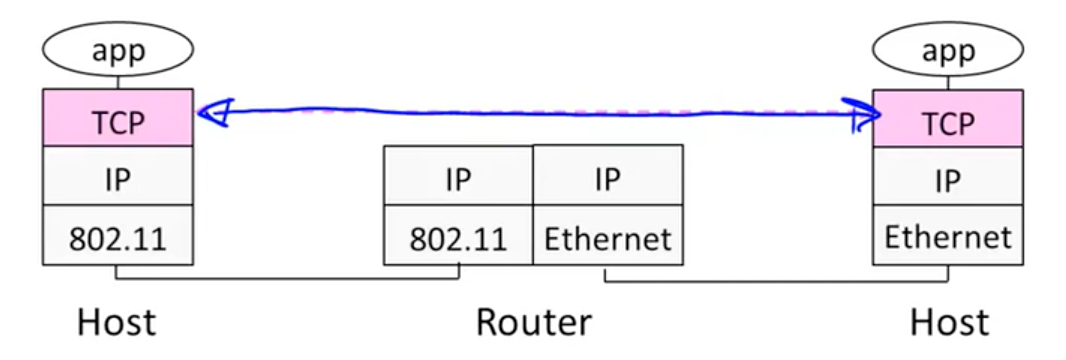
\includegraphics[scale=0.7]{images/6-1-1}
		\caption{ Recall 图一 }
		 \label{fig:6-1-1}
		 \end{figure}
		 
		 \item Segments carry application data across the network
		 \item Segments are carried within packets within frames
		 \item See Figure~\ref{fig:6-1-2}
		 
		 \begin{figure}[h!] % h for here.
		\centering
		 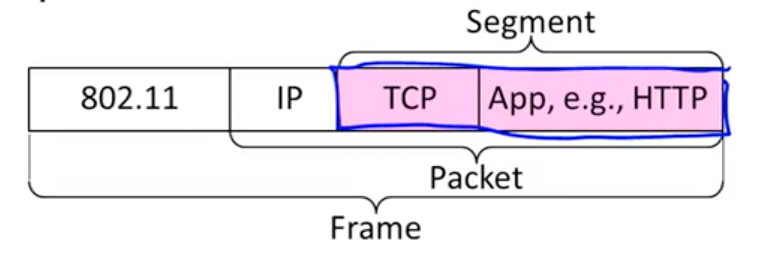
\includegraphics[scale=0.7]{images/6-1-2}
		\caption{ Recall 图二 }
		 \label{fig:6-1-2}
		 \end{figure}
	\end{itemize}
	
	\subsection{Transport Layer Services}
	\begin{itemize}
		\item Provide different kinds of data delivery across the network to applications
		\item See Figure~\ref{fig:6-1-3}
		 
		 \begin{figure}[h!] % h for here.
		\centering
		 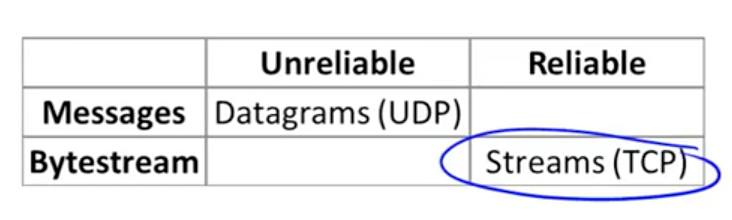
\includegraphics[scale=0.7]{images/6-1-3}
		\caption{ Transport Layer Services }
		 \label{fig:6-1-3}
		 \end{figure}
	\end{itemize}
	
	\subsection{Comparison of Internet Transports}
	\begin{itemize}
		\item TCP is full-featured, UDP is a glorified packet
		\item See Figure~\ref{fig:6-1-4}
		 
		 \begin{figure}[h!] % h for here.
		\centering
		 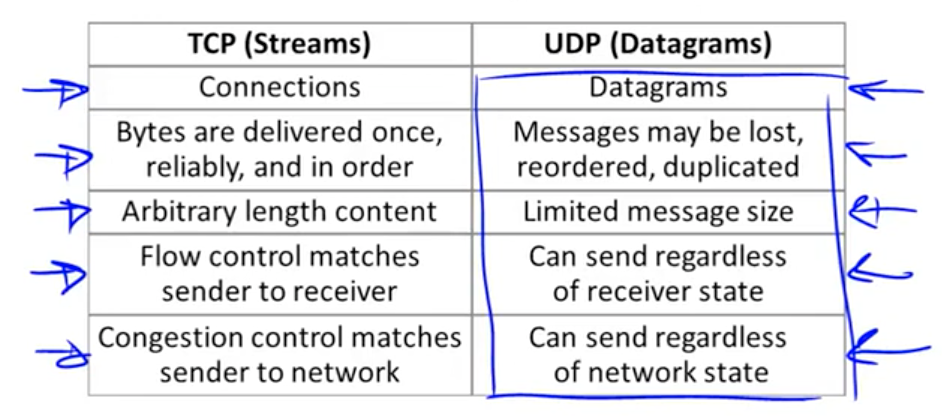
\includegraphics[scale=0.7]{images/6-1-4}
		\caption{ Comparison of Internet Transports }
		 \label{fig:6-1-4}
		 \end{figure}
	\end{itemize}
	
	\subsection{Socket API}
	\begin{itemize}
		\item Simple abstraction to use the network
		\begin{itemize}
			\item The "network" API (really Transport service) used to write all Internet apps
			\item Part of all major OSes and languages; originally Berkeley (Unix) ~1983
		\end{itemize}
		
		\item Supports both Internet transport services (Streams and Datagrams)
		
		\item \underline{Sockets} let apps attach to the local network at different \underline{ports}
		\item See Figure~\ref{fig:6-1-5}
		 
		 \begin{figure}[h!] % h for here.
		\centering
		 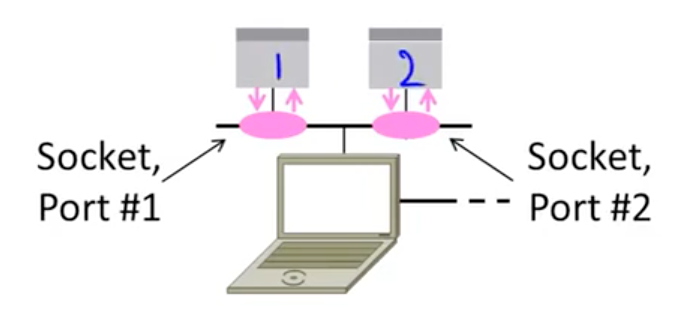
\includegraphics[scale=0.7]{images/6-1-5}
		\caption{ Socket API 图一}
		 \label{fig:6-1-5}
		 \end{figure}
		 
		 \item Same AIP used for streams and Datagrams
		 \item See Figure~\ref{fig:6-1-6}
		 
		 \begin{figure}[h!] % h for here.
		\centering
		 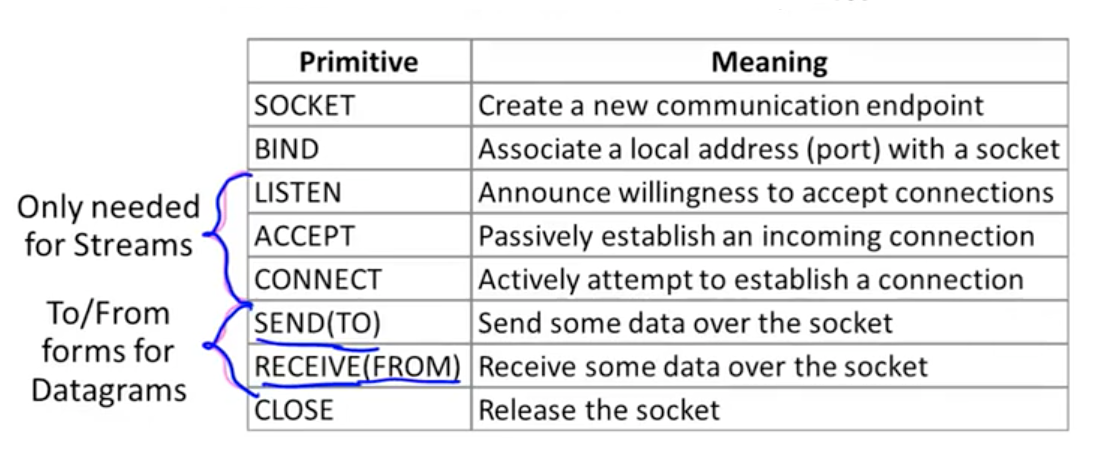
\includegraphics[scale=0.7]{images/6-1-6}
		\caption{ Socket API 图二}
		 \label{fig:6-1-6}
		 \end{figure}
		
	\end{itemize}
	
	\subsection{Ports}
	\begin{itemize}
		\item Application process is identified by the tuple IP address, protocol, and port
		\begin{itemize}
			\item Ports are 16-bit integers representing local "mailboxes" that a process leases(租)
		\end{itemize}
		
		\item Servers often bind to "well-known ports"
		\begin{itemize}
			\item <1024, require administrative privileges
		\end{itemize}
		
		\item Clients often assigned "ephemeral(短暂的)" ports
		\begin{itemize}
			\item Chosen by OS, used temporarily
		\end{itemize}
	\end{itemize}
	
	\subsection{Some Well-Known Ports}
	\begin{itemize}
		\item See Figure~\ref{fig:6-1-7}
		 
		 \begin{figure}[h!] % h for here.
		\centering
		 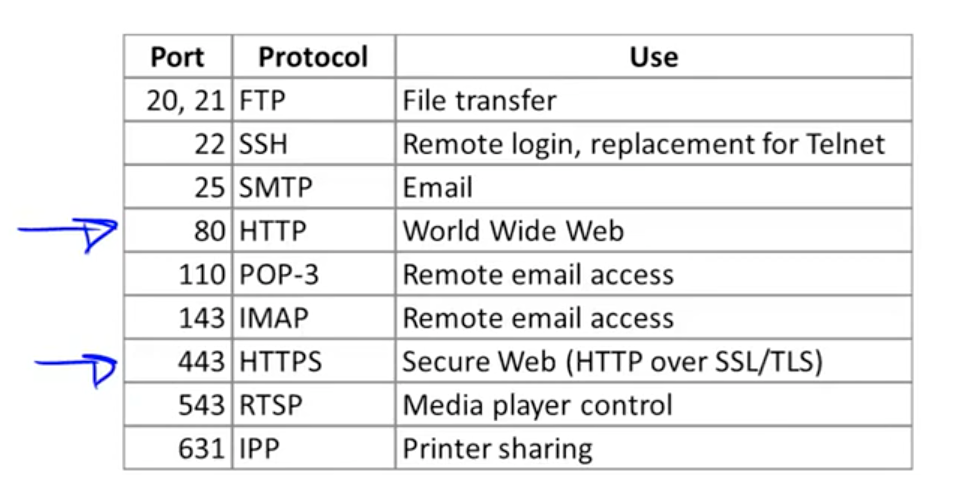
\includegraphics[scale=0.7]{images/6-1-7}
		\caption{ Some Well-Known Ports }
		 \label{fig:6-1-7}
		 \end{figure}
	\end{itemize}
	
	\subsection{Topics}
	\begin{itemize}
		\item {\color{pink} 下面是本次讨论的}
		\item Service models
		\begin{itemize}
			\item Socket API and ports
			\item Datagrams, Streams
		\end{itemize}
		
		\item {\color{pink} 下面是下一次讨论内容}
		\item User Datagram Protocol (UDP)
		\item Connections (TCP)
		\item Sliding Window (TCP)
		\item Flow control (TCP)
		\item Retransmission(中继;转播;重发) timers (TCP)
		
		\item {\color{pink} 下面是再后来谈的内容}
		\item {\color{gray} Congestion control (TCP) }
	\end{itemize}
	
\section{ Week 6.2 - User Datagram Protocol (UDP) }
	\subsection{Topic of UDP}
	\begin{itemize}
		\item Sending messages with UDP
		\begin{itemize}
			\item A shim(用木片或夹铁填孔隙) layer on packets
		\end{itemize}
		\item See Figure~\ref{fig:6-2-1}
		 
		 \begin{figure}[h!] % h for here.
		\centering
		 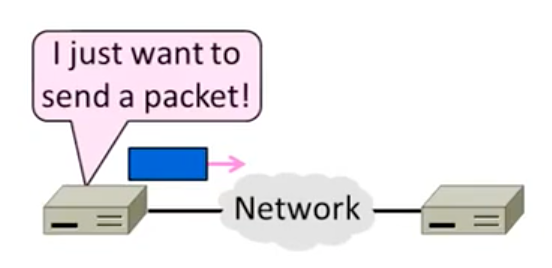
\includegraphics[scale=0.7]{images/6-2-1}
		\caption{ Topic of UDP }
		 \label{fig:6-2-1}
		 \end{figure}
	\end{itemize}
	
	\subsection{ User Datagram Protocol (UDP) }
	\begin{itemize}
		\item Used by apps that don't want reliability or bytestreams
		\begin{itemize}
			\item Voice-over-IP (unreliable)
			\item DNS, RPC (message-oriented)
			\item DHCP (bootstrapping)
		\end{itemize}
		
		\item (If application wants reliability and messages then it has work to do !)
	\end{itemize}
	
	\subsection{ Datagram Sockets }
	\begin{itemize}
		\item See Figure~\ref{fig:6-2-2}
		 
		 \begin{figure}[h!] % h for here.
		\centering
		 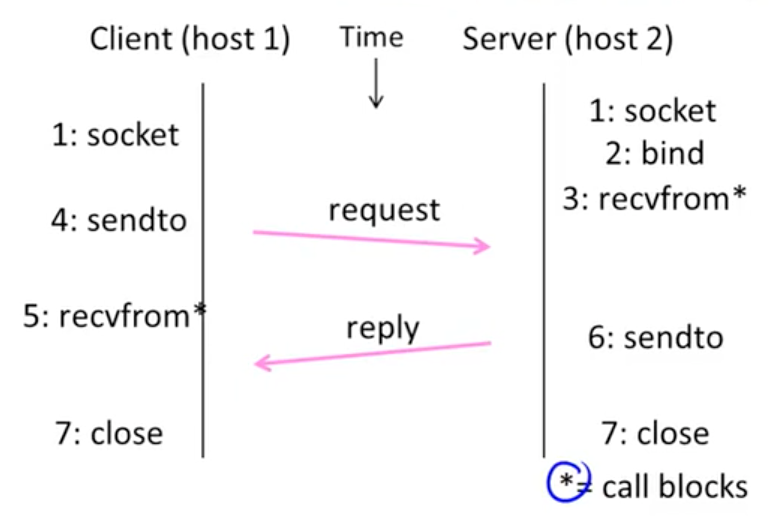
\includegraphics[scale=0.7]{images/6-2-2}
		\caption{ Datagram Sockets }
		 \label{fig:6-2-2}
		 \end{figure}
	\end{itemize}
	
	\subsection{ UDP Buffering }
	\begin{itemize}
		\item 下图中的消息队列就是一个Buffer,接收和发送都是通过消息队列进行的,mux(multiplexer 多路调制器) 和 demex (解调器) 可以把数字量转换为模拟量传送到网络,并在另一个应用的端口进行解调。
		\item See Figure~\ref{fig:6-2-3}
		 
		 \begin{figure}[h!] % h for here.
		\centering
		 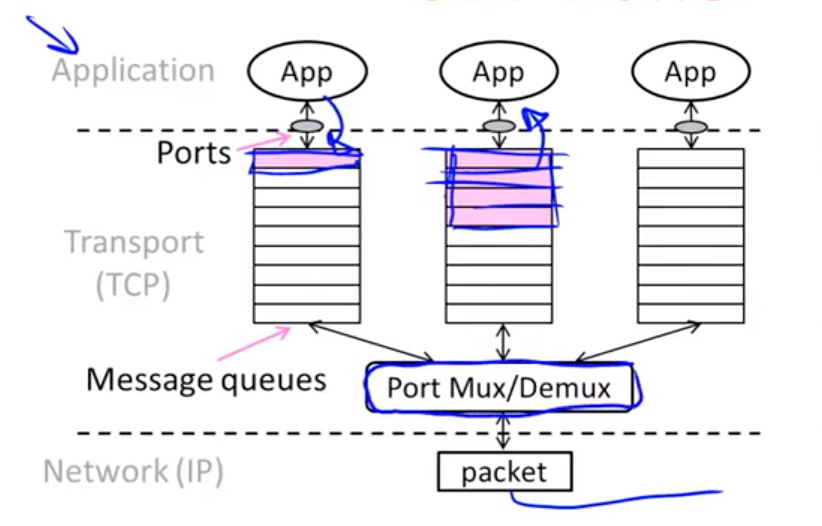
\includegraphics[scale=0.7]{images/6-2-3}
		\caption{ UDP Buffering }
		 \label{fig:6-2-3}
		 \end{figure}
	\end{itemize}
	
	\subsection{UDP Header}
	\begin{itemize}
		\item Uses ports to identify sending and receiving application processes
		\item Datagram length up to 64K
		\item Checksum (16 bits) for reliability
		\item See Figure~\ref{fig:6-2-4}
		 
		 \begin{figure}[h!] % h for here.
		\centering
		 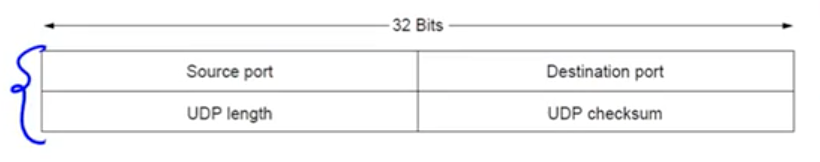
\includegraphics[scale=0.7]{images/6-2-4}
		\caption{ UDP Header 图一 }
		 \label{fig:6-2-4}
		 \end{figure}
		 
		 \item Optional checksum covers UDP segment and IP pseudoheader
		 \begin{itemize}
		 	\item Checks key IP fields (addresses)
		 	\item Value of zero (全零) means "no checksum"
		 \end{itemize}
		 \item See Figure~\ref{fig:6-2-5}
		 
		 \begin{figure}[h!] % h for here.
		\centering
		 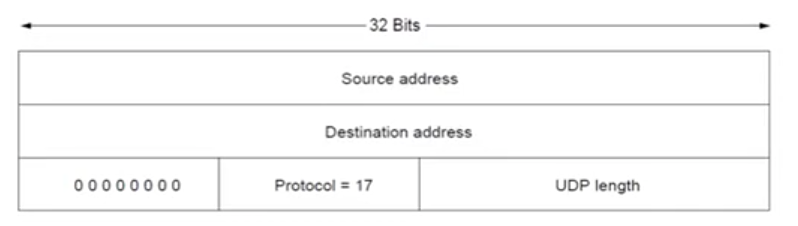
\includegraphics[scale=0.7]{images/6-2-5}
		\caption{ UDP Header 图二 }
		 \label{fig:6-2-5}
		 \end{figure}

	\end{itemize}
	
\section{ Week 6.3 - Connection Establishment }	
	\subsection{Topic of Connection Establishment}
	\begin{itemize}
		\item How to set up connections
		\begin{itemize}
			\item We'll see how does it
		\end{itemize}
		 \item See Figure~\ref{fig:6-3-1}
		 
		 \begin{figure}[h!] % h for here.
		\centering
		 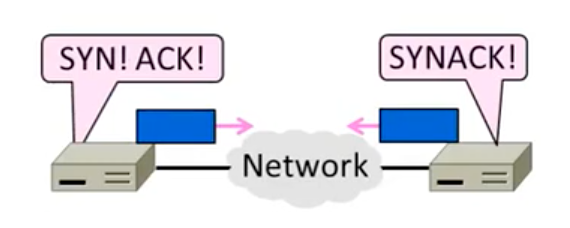
\includegraphics[scale=0.7]{images/6-3-1}
		\caption{ Topic of Connection Establishment }
		 \label{fig:6-3-1}
		 \end{figure}
	\end{itemize}
	
	\subsection{Connection Establishment}
	\begin{itemize}
		\item Both sender and receiver must be ready before we start the transfer of data
		\begin{itemize}
			\item Need to agree on a set of parameters
			\item e.g., the Maximum Segment Size (MSS)
		\end{itemize}
		
		\item This is signaling
		\begin{itemize}
			\item It sets up state at the endpoints
			\item Like "dialing" for a telephone call
		\end{itemize}
	\end{itemize}
	
	\subsection{Three-Way Handshake}
	\begin{itemize}
		\item Used in TCP; opens connection for data in both directions
		\item Each side probes(探测) the other with a fresh Initial Sequence Number (ISN)
		\begin{itemize}
			\item Sends on a SYNchronize(使同步) segment
			\item Echo on an ACKnowlege(告知收到) segment
		\end{itemize}
		
		\item Chosen to be robust event against delayed duplicates
		
		\item Three steps:
		\begin{itemize}
			\item Client sends SYN(x)
			\item Server replies with SYN(y) ACK(x+1)
			\item Client replies with ACK(y+1)
			\item SYNs are retransmitted if lost
		\end{itemize}
		
		\item Sequence and ack numbers carried on further segments
		\item See Figure~\ref{fig:6-3-2}
		 
		 \begin{figure}[h!] % h for here.
		\centering
		 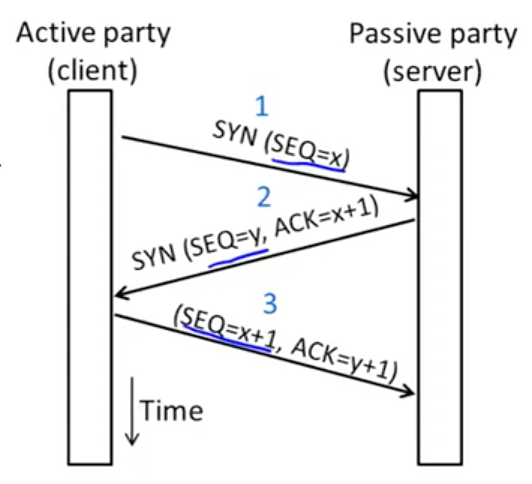
\includegraphics[scale=0.7]{images/6-3-2}
		\caption{ Three-Way Handshake 图一 }
		 \label{fig:6-3-2}
		 \end{figure}
		 
		 \item Suppose delayed, duplicate copies of the SYN and ACK arrive at the server!
		 \begin{itemize}
		 	\item Improbable(不像会发生的), but anyhow(不管怎样) ...
		 	\item client 和 server 会拒绝这样的signal。
		 \end{itemize}
		 \item See Figure~\ref{fig:6-3-3}
		 
		 \begin{figure}[h!] % h for here.
		\centering
		 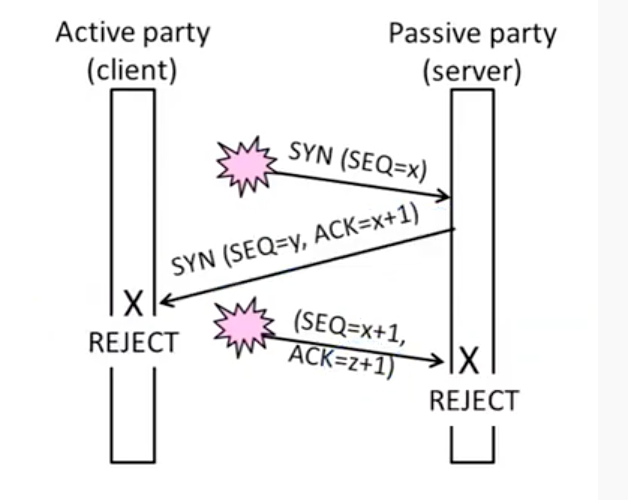
\includegraphics[scale=0.7]{images/6-3-3}
		\caption{ Three-Way Handshake 图二 }
		 \label{fig:6-3-3}
		 \end{figure}

		 \item Connection will be cleanly rejected on both sides
	\end{itemize}
	
	\subsection{TCP Connection State Machine}
	\begin{itemize}
		\item Captures the states (rectangles) and transitions (arrows)
		\begin{itemize}
			\item A/B means event A triggers(触发) the transition(转变), with action B
			\item 比如下图 CONNECT 触发使得发出SYS(Step1  of the 3-way handshake) ,注意:在Client和Server都运行这个状态机
		\end{itemize}
		
		\item Follow the path of the client:
		\item See Figure~\ref{fig:6-3-4}
		 
		 \begin{figure}[h!] % h for here.
		\centering
		 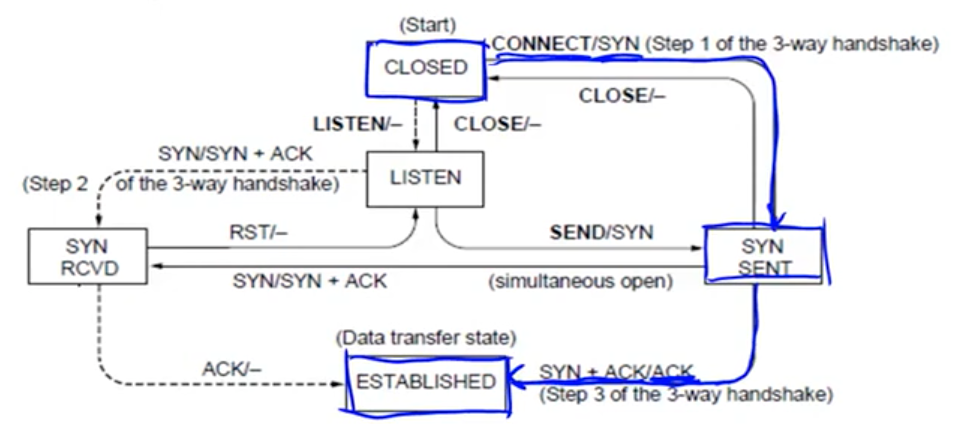
\includegraphics[scale=0.7]{images/6-3-4}
		\caption{ TCP Connection State Machine 图一 }
		 \label{fig:6-3-4}
		 \end{figure}
		 
		 \item And the path of the server:
		 \item See Figure~\ref{fig:6-3-5}
		 
		 \begin{figure}[h!] % h for here.
		\centering
		 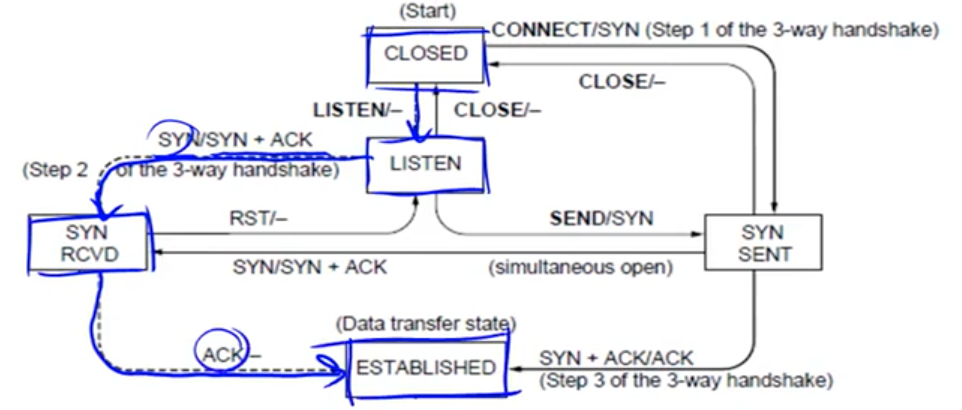
\includegraphics[scale=0.7]{images/6-3-5}
		\caption{ TCP Connection State Machine 图二 }
		 \label{fig:6-3-5}
		 \end{figure}
		 
		 \item Again, with states ...
		  \item See Figure~\ref{fig:6-3-6}
		 
		 \begin{figure}[h!] % h for here.
		\centering
		 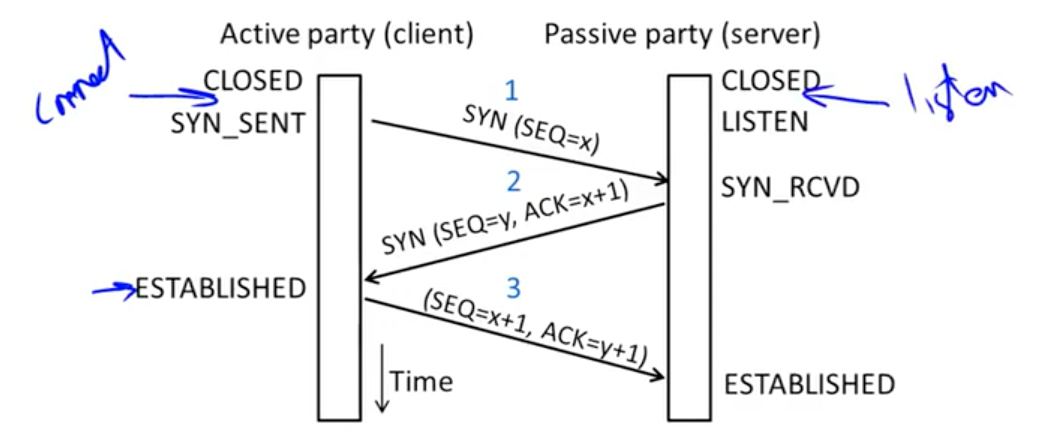
\includegraphics[scale=0.7]{images/6-3-6}
		\caption{ TCP Connection State Machine 图三 }
		 \label{fig:6-3-6}
		 \end{figure}
		 
		 \item Finite state machines are a useful tool to specify and check the handling of all cases the may occur
		 
		 \item TCP allows for simultaneous open
		 \begin{itemize}
		 	\item i.e., both sides open at once instead of the client-server pattern
		 	\item Try at home to confirm it works
		 \end{itemize}
		
	\end{itemize}
	
\section{ Week 6.4 - Connection Release }
	\subsection{ Topic of Connection Release }
	\begin{itemize}
		\item How to release connections
		\begin{itemize}
			\item We'll see how TCP does it
		\end{itemize}
		 \item See Figure~\ref{fig:6-4-1}
		  
		 \begin{figure}[h!] % h for here.
		\centering
		 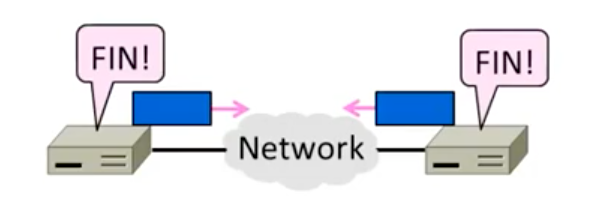
\includegraphics[scale=0.7]{images/6-4-1}
		\caption{  Topic of Connection Release }
		 \label{fig:6-4-1}
		 \end{figure}
	\end{itemize}
	
	\subsection{Connection Release}
	\begin{itemize}
		\item Orderly release by both parties when done
		\begin{itemize}
			\item Delivers all pending data and "hangs up"
			\item Cleans up state in sender and receiver
		\end{itemize}
		
		\item Key problem is to provide reliability while releasing
		\begin{itemize}
			\item TCP uses a "symmetric" close in which both sides shutdown independently
		\end{itemize}
	\end{itemize}
	
	\subsection{TCP Connection Release}
	\begin{itemize}
		\item Two steps:
		\begin{itemize}
			\item Active sends FIN(x), passive ACKs
			\item Passive sends FIN(y), active ACKs
			\item FINs are retransmitted if lost
		\end{itemize}
		
		\item Each FIN/ACK closes one direction of data transfer
		 \item See Figure~\ref{fig:6-4-2}
		  
		 \begin{figure}[h!] % h for here.
		\centering
		 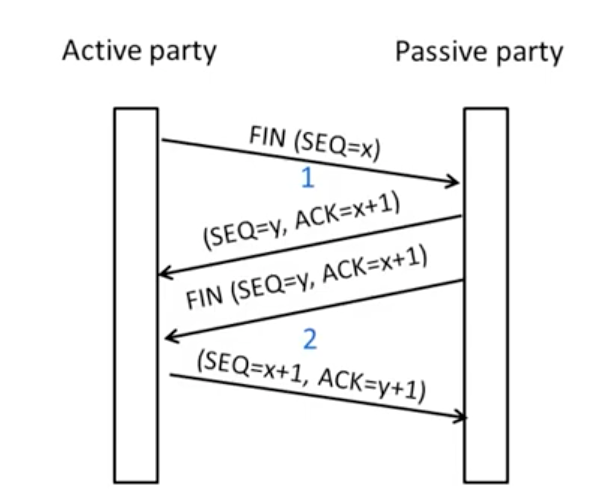
\includegraphics[scale=0.7]{images/6-4-2}
		\caption{  TCP Connection Release }
		 \label{fig:6-4-2}
		 \end{figure}
	\end{itemize}
	
	\subsection{TCP Connection State Machine}
	\begin{itemize}
		 \item See Figure~\ref{fig:6-4-3}
		  
		 \begin{figure}[h!] % h for here.
		\centering
		 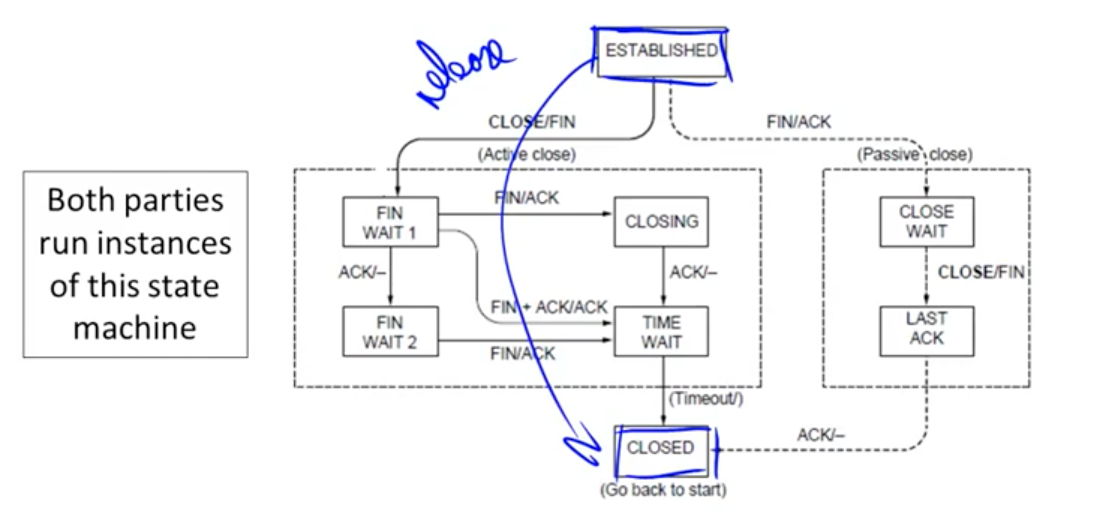
\includegraphics[scale=0.7]{images/6-4-3}
		\caption{  TCP Connection State Machine }
		 \label{fig:6-4-3}
		 \end{figure}
	\end{itemize}
	
	\subsection{TCP Release}
	\begin{itemize}
		\item Follow the active party
		\item See Figure~\ref{fig:6-4-4}
		  
		 \begin{figure}[h!] % h for here.
		\centering
		 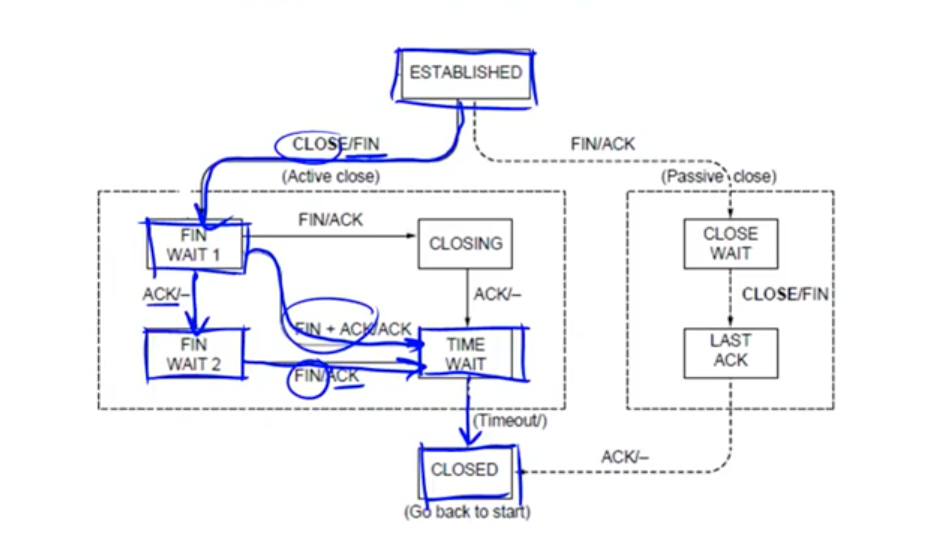
\includegraphics[scale=0.7]{images/6-4-4}
		\caption{  TCP Release 图一 }
		 \label{fig:6-4-4}
		 \end{figure}
		 
		 \item Follow the passive party
		 \item See Figure~\ref{fig:6-4-5}
		  
		 \begin{figure}[h!] % h for here.
		\centering
		 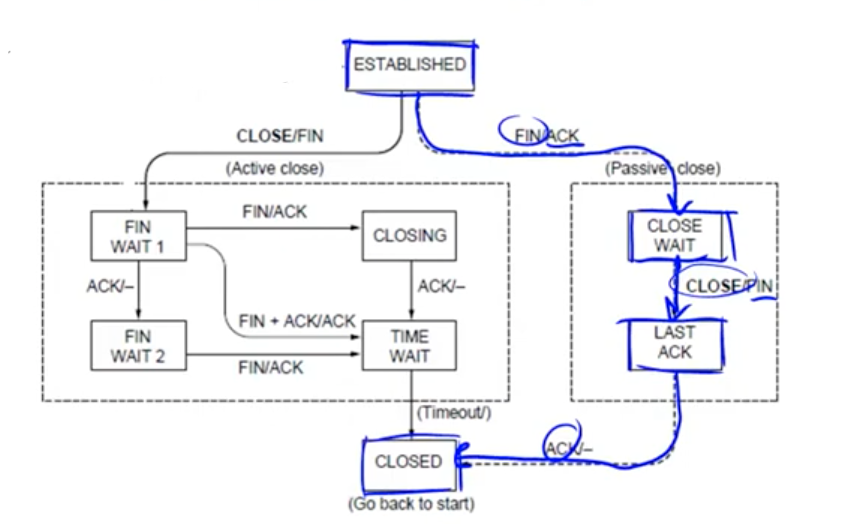
\includegraphics[scale=0.7]{images/6-4-5}
		\caption{  TCP Release 图二 }
		 \label{fig:6-4-5}
		 \end{figure}
		 
		 \item Again, with states ...
		 \item See Figure~\ref{fig:6-4-6}
		  
		 \begin{figure}[h!] % h for here.
		\centering
		 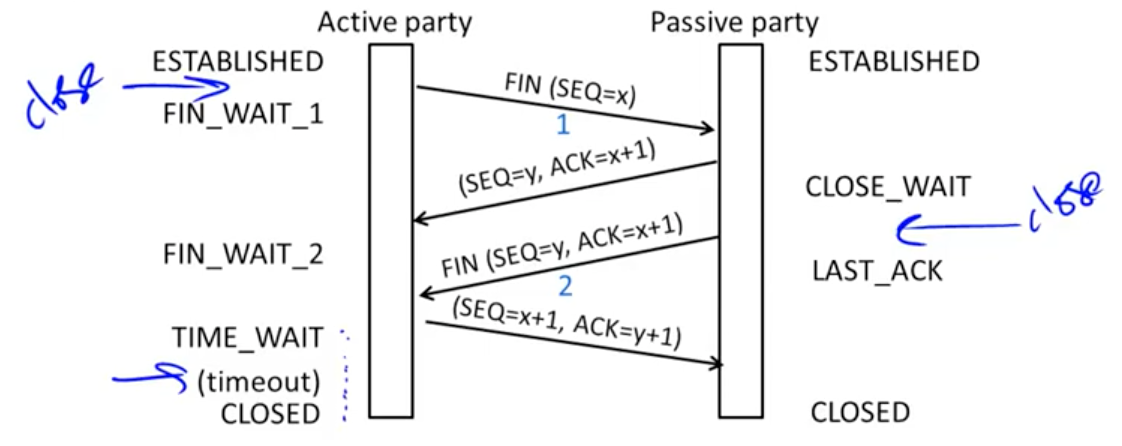
\includegraphics[scale=0.7]{images/6-4-6}
		\caption{  TCP Release 图三 }
		 \label{fig:6-4-6}
		 \end{figure}

	\end{itemize}
	
	\subsection{TIME\_WAIT State}
	\begin{itemize}
		\item We wait a long time (two times the maximum segment lifetime of 60 seconds) after sending all segments and before completing the close
		\item Why?
		\begin{itemize}
			\item ACK might have been lost, in which case FIN will be resent for an orderly close
			\item Could otherwise interfere(干涉;妨碍) with a subsequent connection
		\end{itemize}
	\end{itemize}
	

\section{Week 6.5 - Sliding Window}
	\subsection{Topic of Sliding Window}
	\begin{itemize}
		\item The sliding window algorithm
		\begin{itemize}
			\item Pipelining and reliability
			\item Building on Stop-and-Wait
		\end{itemize}
		 \item See Figure~\ref{fig:6-5-1}
		  
		 \begin{figure}[h!] % h for here.
		\centering
		 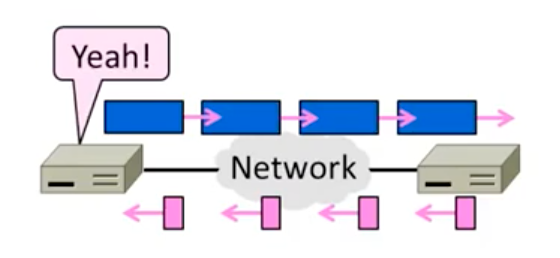
\includegraphics[scale=0.7]{images/6-5-1}
		\caption{  Topic of Sliding Window }
		 \label{fig:6-5-1}
		 \end{figure}
	\end{itemize}
	
	\subsection{Recall}
	\begin{itemize}
		\item ARQ with one message at a time is Stop-and-Wait (normal case below)
		\item See Figure~\ref{fig:6-5-2}
		  
		 \begin{figure}[h!] % h for here.
		\centering
		 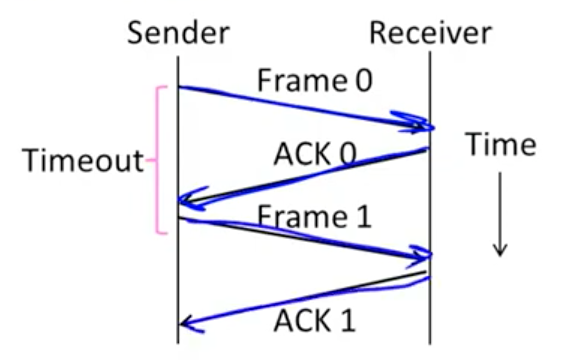
\includegraphics[scale=0.7]{images/6-5-2}
		\caption{  Recall }
		 \label{fig:6-5-2}
		 \end{figure}
	\end{itemize}
	
	\subsection{Limitation of Stop-and-Wait}
	\begin{itemize}
		\item It allows only a single message to be outstanding from the sender:
		\begin{itemize}
			\item Fine for LAN (only one frame fit)
			\item Not efficient for network paths with BD >> 1 packet
		\end{itemize}
		
		\item Example: R=1 Mbps, D=50 ms
		\begin{itemize}
			\item RTT (Round Trip Time) = 2D = 100 ms
			\item How meny packets/sec ?
			\begin{itemize}
				\item 10 packets/sec = 100 kbps (~10\%)
			\end{itemize}
			\item What if R=10 Mbps?
			\begin{itemize}
				\item 10 packets/sec = 100 kbps (~1\%)
			\end{itemize}
		\end{itemize}
	\end{itemize}
	
	\subsection{Sliding Window}
	\begin{itemize}
		\item Generalization of stop-and-wait
		\begin{itemize}
			\item Allow W packets to be outstanding
			\item Can send W packets per RTT (2D)
			\item \underline{Pipelining} improves performance
			\item Need W=2BD to fill network path
		\end{itemize}
		\item See Figure~\ref{fig:6-5-3}
		  
		 \begin{figure}[h!] % h for here.
		\centering
		 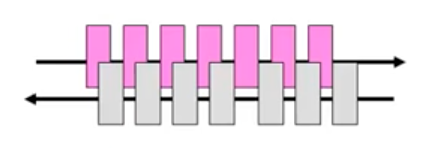
\includegraphics[scale=0.7]{images/6-5-3}
		\caption{  Sliding Window }
		 \label{fig:6-5-3}
		 \end{figure}
		 
		 \item What W will use the network capacity?
		 \item Ex: R=1 Mbps, D=50 ms
		 \begin{itemize}
		 	\item W = 2BD = $10^{6} * 100 * 10^{-3}$ = 100Kb $\approx$ 10 packets
		 \end{itemize}
		 
		 \item Ex: What if R=10 Mbps?
		 \begin{itemize}
		 	\item W=2BD = 1000 Kb $\approx$ 100 packets
		 \end{itemize}
	\end{itemize}
	
	\subsection{Sliding Window Protocol}
	\begin{itemize}
		\item Many variations, depending on how buffers, acknowledgements, and retransmissions are handled
		
		\item \underline{Go-Back-N}
		\begin{itemize}
			\item Simplest version, can be inefficient
		\end{itemize}
		
		\item \underline{Selective Repeat}
		\begin{itemize}
			\item More complex, better performance
		\end{itemize}
	\end{itemize}
	
	\subsection{Sliding Window - Sender}
	\begin{itemize}
		\item Sender buffers up to W segments until they are acknowledged
		\begin{itemize}
			\item LFS=LAST FRAME SENT, LAR=LAST ACK REC'D
			\item Sends while $LFS - LAR \leq W$
		\end{itemize}
		\item See Figure~\ref{fig:6-5-4}
		  
		 \begin{figure}[h!] % h for here.
		\centering
		 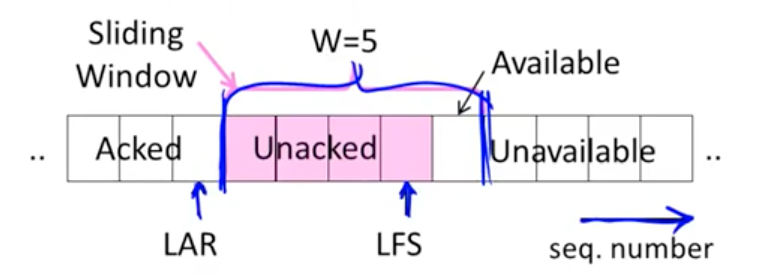
\includegraphics[scale=0.7]{images/6-5-4}
		\caption{  Sliding Window - Sender 图一}
		 \label{fig:6-5-4}
		 \end{figure}
		 
		 \item Transport accepts another segment of data from the Application ...
		 \begin{itemize}
		 	\item Transport sends it (as $LFS - LAR \rightarrow 5$)
		 \end{itemize}
		 \item See Figure~\ref{fig:6-5-5}
		  
		 \begin{figure}[h!] % h for here.
		\centering
		 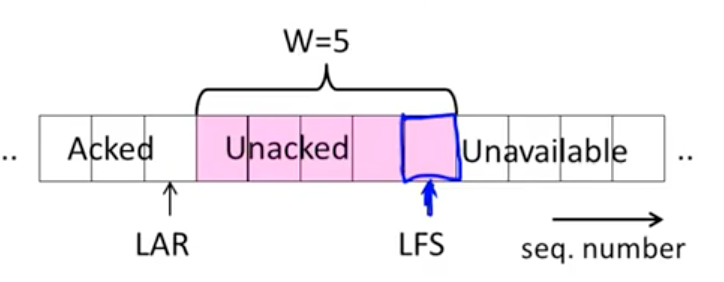
\includegraphics[scale=0.7]{images/6-5-5}
		\caption{  Sliding Window - Sender 图二}
		 \label{fig:6-5-5}
		 \end{figure}
		 
		 \item Next higher ACK arrives from peer ...
		 \begin{itemize}
		 	\item Window advances, buffer is freed
		 	\item $LFS - LAR \rightarrow 4$ (can send one more)
		 \end{itemize}
		  \item See Figure~\ref{fig:6-5-6}
		  
		 \begin{figure}[h!] % h for here.
		\centering
		 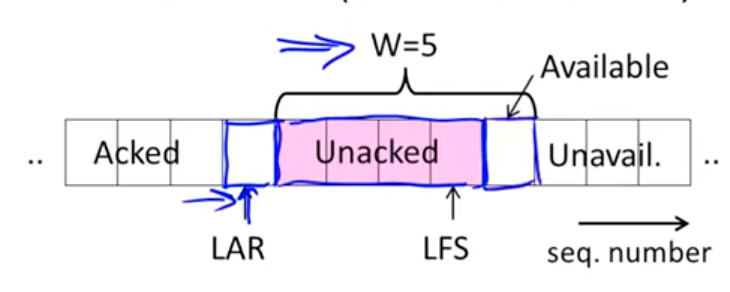
\includegraphics[scale=0.7]{images/6-5-6}
		\caption{  Sliding Window - Sender 图三}
		 \label{fig:6-5-6}
		 \end{figure}
		 
	\end{itemize}
	
	\subsection{Sliding Window - Go-Back-N}
	\begin{itemize}
		\item Receiver keeps only a single packet buffer for the next segment
		\begin{itemize}
			\item State variable, LAS = LAST ACK SENT
		\end{itemize}
		
		\item On receive:
		\begin{itemize}
			\item If seq. number is LAS+1, accept and pass it to app, update LAS, send ACK
			\item Otherwise discard (as out of order)
		\end{itemize}
	\end{itemize}
	
	\subsection{Sliding Window - Selective Repeat}
	\begin{itemize}
		\item Receiver passes data to app in order, and buffers out-of-order segments to reduce retransmissions
		\item ACK conveys(传达,传输) highest in-order segment, plus hints about out-of-order segments
		\item TCP uses a selective repeat design; we'll see the details later
		
		\item Buffers W segments, keeps state variable, LAS = LAST ACK SENT
		\item On receive:
		\begin{itemize}
			\item Buffer segments [LAS+1, LAS+W]
			\item Pass up to app in-order segments from LAS+1, and update LAS
			\item Send ACK for LAS regardless
		\end{itemize}
	\end{itemize}
	
	\subsection{Sliding Window - Retransmissions}
	\begin{itemize}
		\item Go-Back-N sender uses a single timer to detect loss
		\begin{itemize}
			\item On timeout, resends buffered packets starting at LAR+1
		\end{itemize}
		
		\item Selective Repeat sender uses a timer per unacked segment to detect losses
		\begin{itemize}
			\item On timeout for segment, resend it
			\item Hope to resend fewer segments
		\end{itemize}
	\end{itemize}
	
	\subsection{Sequence Numbers}
	\begin{itemize}
		\item Need more then 0/1 for Stop-and-Wait ...
		\begin{itemize}
			\item But how many?
		\end{itemize}
		
		\item For Selective Repeat, need W numbers for packets, plus W for acks of earlier packets
		\begin{itemize}
			\item 2W seq. numbers
			\item Fewer for Go-Back-N (W+1)
		\end{itemize}
		
		\item Typically implement seq. number with an N-bit counter that wraps around at $2^{N} - 1$
		\begin{itemize}
			\item E.g., N=8: ..., 253, 254, 255, 0, 1, 2, 3, ...
		\end{itemize}
	\end{itemize}
	
	\subsection{Sequence Time Plot}
	\begin{itemize}
		\item See Figure~\ref{fig:6-5-7}
		  
		 \begin{figure}[h!] % h for here.
		\centering
		 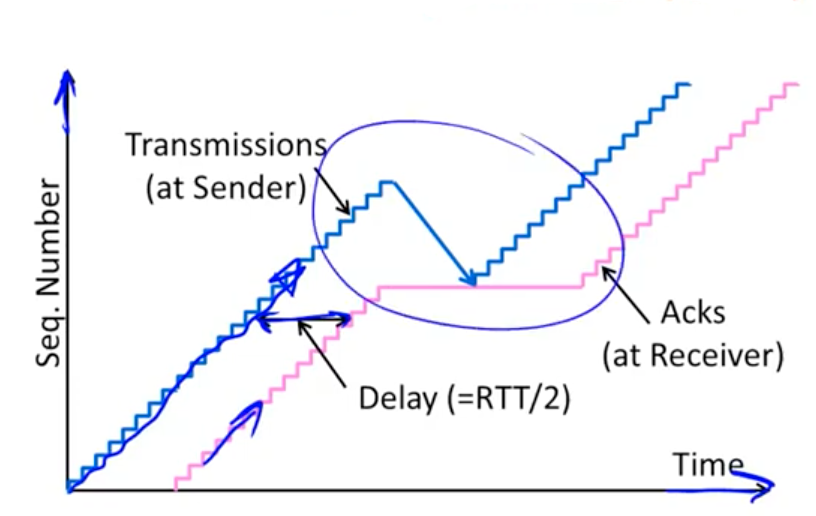
\includegraphics[scale=0.7]{images/6-5-7}
		\caption{  Sequence Time Plot 图一}
		 \label{fig:6-5-7}
		 \end{figure}
		 
		 \item 上面图中的发送端曲折,是由于丢包导致的,下面图作一个分析。
		 \item See Figure~\ref{fig:6-5-8}
		  
		 \begin{figure}[h!] % h for here.
		\centering
		 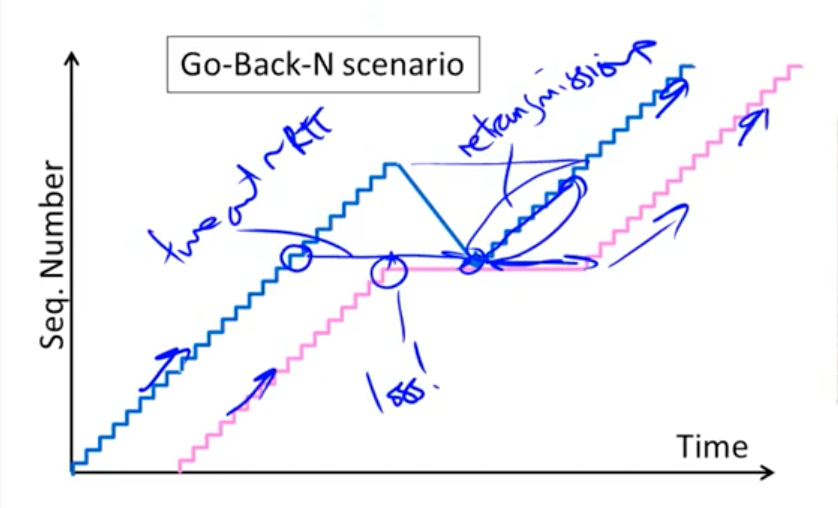
\includegraphics[scale=0.7]{images/6-5-8}
		\caption{  Sequence Time Plot 图二}
		 \label{fig:6-5-8}
		 \end{figure}
	\end{itemize}
	
\section{Week 6.6 - Flow Control}
	\subsection{Topic of Flow Control}
	\begin{itemize}
		\item Adding flow control to the sliding window algorithm
		\begin{itemize}
			\item To slow the over-enthusiastic sender
		\end{itemize}
		\item See Figure~\ref{fig:6-6-1}
		  
		 \begin{figure}[h!] % h for here.
		\centering
		 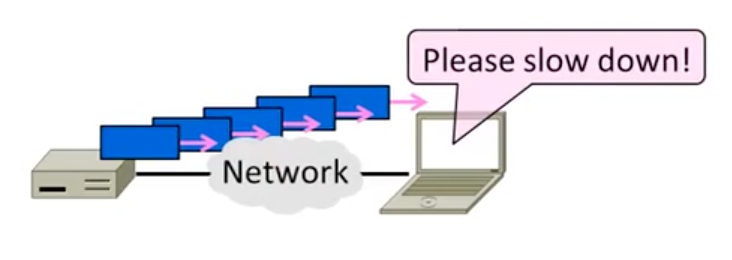
\includegraphics[scale=0.7]{images/6-6-1}
		\caption{  Topic of Flow Control }
		 \label{fig:6-6-1}
		 \end{figure}
	\end{itemize}
	
	\subsection{Problem}
	\begin{itemize}
		\item Sliding window uses pipelining to keep the network busy
		\begin{itemize}
			\item What if the receiver is overloaded?
		\end{itemize}
		\item See Figure~\ref{fig:6-6-2}
		  
		 \begin{figure}[h!] % h for here.
		\centering
		 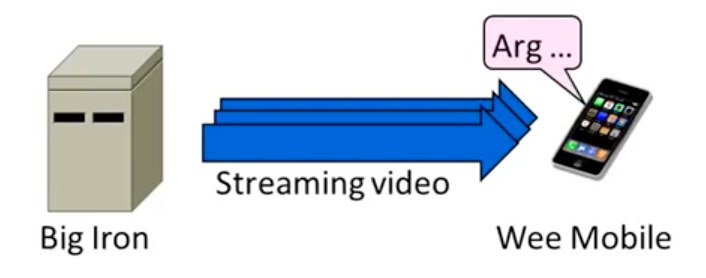
\includegraphics[scale=0.7]{images/6-6-2}
		\caption{  Problem }
		 \label{fig:6-6-2}
		 \end{figure}
	\end{itemize}
	
	\subsection{Sliding Window - Receiver}
	\begin{itemize}
	 	\item Consider receiver with W buffers
	 	\begin{itemize}
	 		\item LAS=LAST ACK SENT, app pulls in-order data from buffer with recv() call
	 	\end{itemize}
	 	\item See Figure~\ref{fig:6-6-3}
		  
		 \begin{figure}[h!] % h for here.
		\centering
		 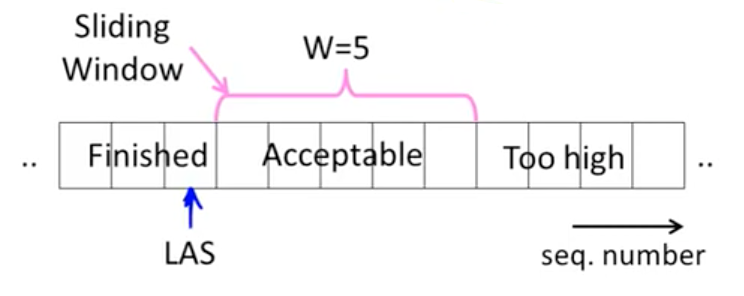
\includegraphics[scale=0.7]{images/6-6-3}
		\caption{  Sliding Window - Receiver 图一 }
		 \label{fig:6-6-3}
		 \end{figure}
		 
		 \item Suppose the next two segments arrive but app does not call recv()
		 \begin{itemize}
		 	\item LAS rises, but we can't slide window!
		 \end{itemize}
		 \item See Figure~\ref{fig:6-6-4}
		  
		 \begin{figure}[h!] % h for here.
		\centering
		 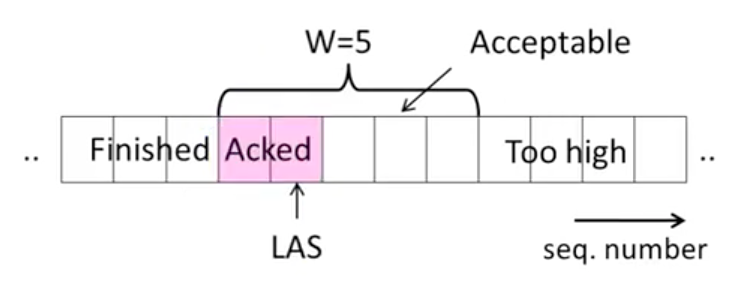
\includegraphics[scale=0.7]{images/6-6-4}
		\caption{  Sliding Window - Receiver 图二 }
		 \label{fig:6-6-4}
		 \end{figure}
		 
		 \item If further segments arrive (even in order) we can fill the buffer
		 \begin{itemize}
		 	\item Must drop segments until app recvs!
		 \end{itemize}
		 \item See Figure~\ref{fig:6-6-5}
		  
		 \begin{figure}[h!] % h for here.
		\centering
		 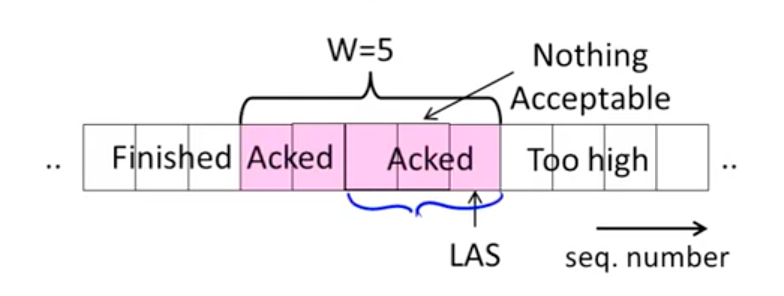
\includegraphics[scale=0.7]{images/6-6-5}
		\caption{  Sliding Window - Receiver 图三 }
		 \label{fig:6-6-5}
		 \end{figure}
		 
		 \item App recv() takes two segments
		 \begin{itemize}
		 	\item Window slides (phew很慢很慢)
		 \end{itemize}
		  \item See Figure~\ref{fig:6-6-6}
		  
		 \begin{figure}[h!] % h for here.
		\centering
		 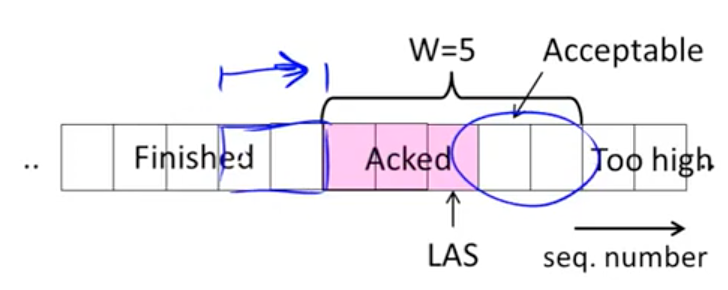
\includegraphics[scale=0.7]{images/6-6-6}
		\caption{  Sliding Window - Receiver 图四 }
		 \label{fig:6-6-6}
		 \end{figure}
		
	\end{itemize}
	
	\subsection{Flow Control}
	\begin{itemize}
		\item Avoid loss at receiver by telling sender the available buffer space
		\begin{itemize}
			\item WIN=\#Acceptable, not W (from LAS)
		\end{itemize}
		\item See Figure~\ref{fig:6-6-7}
		  
		 \begin{figure}[h!] % h for here.
		\centering
		 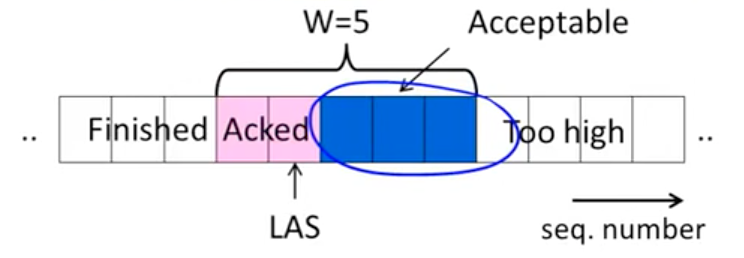
\includegraphics[scale=0.7]{images/6-6-7}
		\caption{ Flow Control 图一  }
		 \label{fig:6-6-7}
		 \end{figure}
		 
		 \item Sender uses the lower of the sliding window and \underline{flow control window} (WIN) as the effective window size
		 \item See Figure~\ref{fig:6-6-8}
		  
		 \begin{figure}[h!] % h for here.
		\centering
		 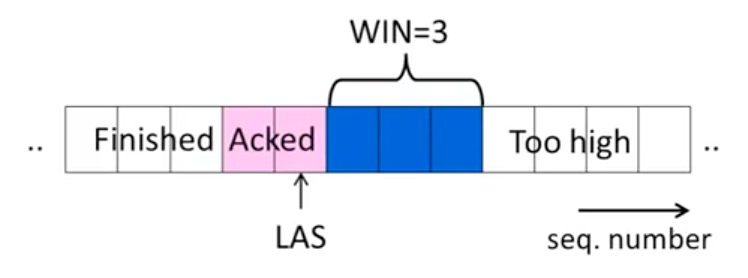
\includegraphics[scale=0.7]{images/6-6-8}
		\caption{ Flow Control 图二  }
		 \label{fig:6-6-8}
		 \end{figure}
		 
		 \item TCP-style example
		 \begin{itemize}
		 	\item SEQ/ACK sliding window
		 	\item Flow control with WIN
		 	\item SEQ + length < ACK + WIN
		 	\item 4KB buffer at receiver
		 	\item Circular buffer of bytes
		 \end{itemize}
		  \item See Figure~\ref{fig:6-6-9}
		  
		 \begin{figure}[h!] % h for here.
		\centering
		 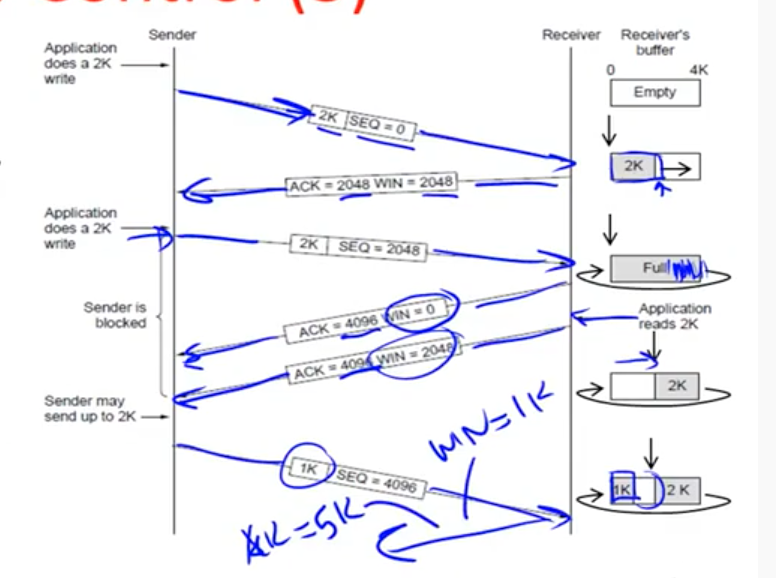
\includegraphics[scale=0.7]{images/6-6-9}
		\caption{ Flow Control 图三  }
		 \label{fig:6-6-9}
		 \end{figure}
	\end{itemize}
	
\section{Week 6.7 - Retransmission Timeouts}
	\subsection{Topic of Retransmission Timeouts}
	\begin{itemize}
		\item How to set the timeout for sending a retransmission
		\begin{itemize}
			\item Adapting to the network path
		\end{itemize}
		 \item See Figure~\ref{fig:6-7-1}
		  
		 \begin{figure}[h!] % h for here.
		\centering
		 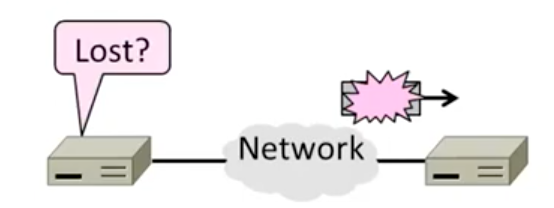
\includegraphics[scale=0.7]{images/6-7-1}
		\caption{ Topic of Retransmission Timeouts  }
		 \label{fig:6-7-1}
		 \end{figure}
	\end{itemize}
	
	\subsection{Retransmissions}
	\begin{itemize}
		\item With sliding window, the strategy for detecting loss is the \underline{timeout}
		\begin{itemize}
			\item Set timer when a segment is sent
			\item Cancel timer when ack is received
			\item If timer fires, \underline{retransmit} data as lost
		\end{itemize}
		\item See Figure~\ref{fig:6-7-2}
		  
		 \begin{figure}[h!] % h for here.
		\centering
		 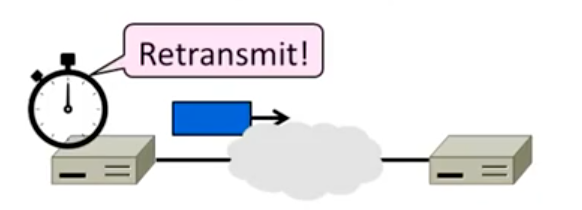
\includegraphics[scale=0.7]{images/6-7-2}
		\caption{ Retransmissions  }
		 \label{fig:6-7-2}
		 \end{figure}
	\end{itemize}
	
	\subsection{Timeout Problem}
	\begin{itemize}
		\item Timeout should be "just right"
		\begin{itemize}
			\item Too long wastes network capacity
			\item Too short leads to spurious(伪) resends
		\end{itemize}
		
		\item Easy to set on a LAN (Link)
		\begin{itemize}
			\item Short, fixed, predictable RTT
		\end{itemize}
		
		\item Hard on the Internet (Transport)
		\begin{itemize}
			\item Wide range, variable RTT
		\end{itemize}
	\end{itemize}
	
	\subsection{Example of RTTs}
	\begin{itemize}
		\item 下面这幅图描述了从Barcelona到海外再回来这个回路的RTTs
		\item See Figure~\ref{fig:6-7-3}
		  
		 \begin{figure}[h!] % h for here.
		\centering
		 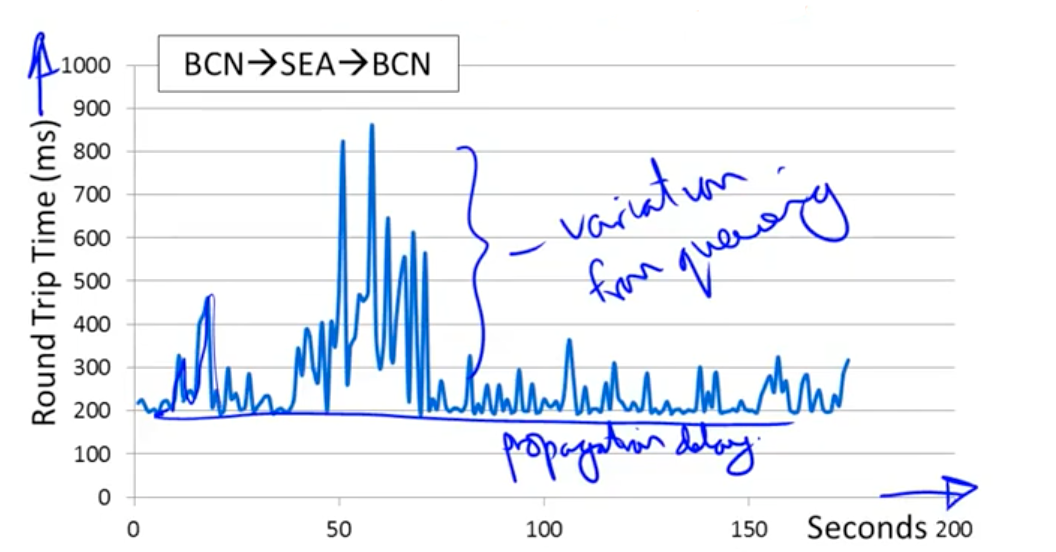
\includegraphics[scale=0.7]{images/6-7-3}
		\caption{ Example of RTTs 图一 }
		 \label{fig:6-7-3}
		 \end{figure}
		
		\item 下面进一步的说明
		\item See Figure~\ref{fig:6-7-4}
		  
		 \begin{figure}[h!] % h for here.
		\centering
		 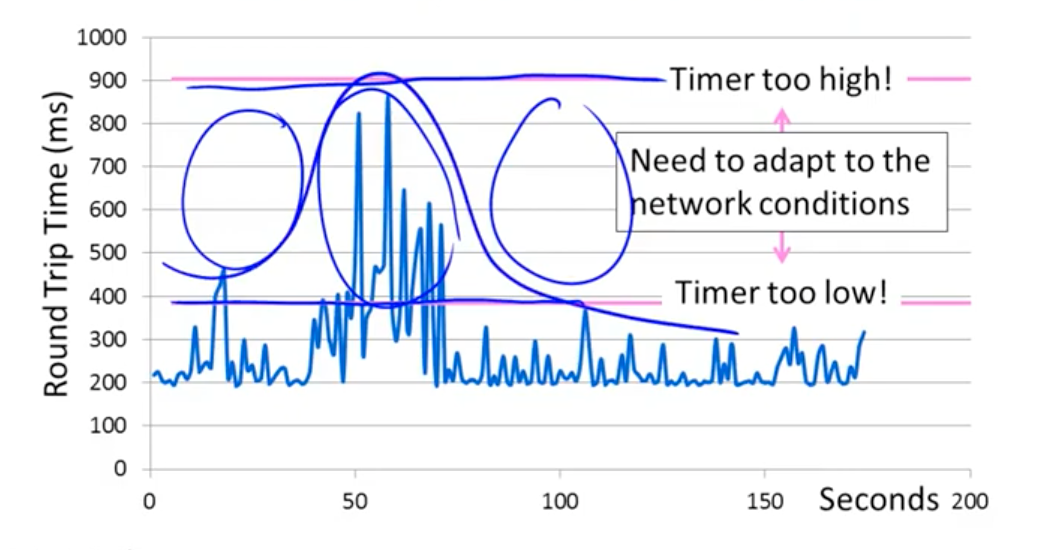
\includegraphics[scale=0.7]{images/6-7-4}
		\caption{ Example of RTTs 图二 }
		 \label{fig:6-7-4}
		 \end{figure}
	\end{itemize}
	
	\subsection{Adaptive Timeout}
	\begin{itemize}
		\item Keep smoothed estimates of the RTT({\color{blue} 1}) and variance in RTT ({\color{blue} 2})
		\begin{itemize}
			\item Update estimates with a moving average
			\item {\color{blue} 1.} $SRTT_{N+1} = 0.9*SRTT_{N} + 0.1*RTT_{N+1}$
			\item {\color{blue} 2.} $Svar_{N+1} = 0.9*Svar_{N} + 0.1*|RTT_{N+1} - SRTT_{N+1}|$
		\end{itemize}
		
		\item Set timeout to a multiple of estimates
		\begin{itemize}
			\item To estimate the upper RTT in practice
			\item TCP $Timeout_{N} = SRTT_{N} + 4*Svar_{N}$
		\end{itemize}
		
		\item Simple to compute, does a good job of tracking actual RTT
		\begin{itemize}
			\item Little "headroom"(上升空间) to lower
			\item Yet very few early timeouts
		\end{itemize}
		
		\item Turns out to be important for good performance and robustness
	\end{itemize}
	
	\subsection{Example of Adaptive Timeout}
	\begin{itemize}
		\item 下图符合公式 $Timeout_{N} = SRTT_{N} + 4*Svar_{N}$
		\item See Figure~\ref{fig:6-7-5}
		  
		 \begin{figure}[h!] % h for here.
		\centering
		 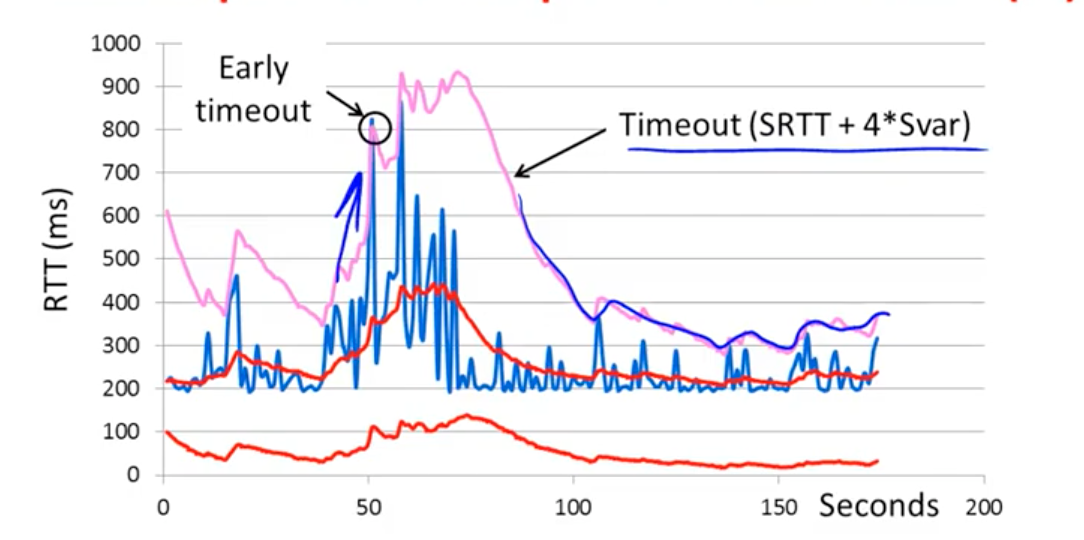
\includegraphics[scale=0.7]{images/6-7-5}
		\caption{ Example of Adaptive Timeout }
		 \label{fig:6-7-5}
		 \end{figure}
	\end{itemize}
	
\section{Week 6.8 - Transmission Control Protoco TCP}
	\subsection{Topic of TCP }
	\begin{itemize}
		\item How TCP works!
		\begin{itemize}
			\item The transport protocol used for most content on the Internet
		\end{itemize}
	\end{itemize}
	
	\subsection{TCP Features}
	\begin{itemize}
		\item {\color{red} 本节课内容:}
		\item A reliable bytestream service
		\item Sliding window for reliability
		\begin{itemize}
			\item With adaptive timeout
		\end{itemize}
		\item Flow control for slow receivers
		
		\item {\color{red} 下节课内容:}
		\item Congestion control to allocate network bandwidth
	\end{itemize}
	
	\subsection{Reliable Bytestream}
	\begin{itemize}
		\item Message boundaries(边界) not preserved from send() to recv()
		\begin{itemize}
			\item But reliable and ordered (receive bytes in same order as sent)
		\end{itemize}
		\item See Figure~\ref{fig:6-8-1}
		  
		 \begin{figure}[h!] % h for here.
		\centering
		 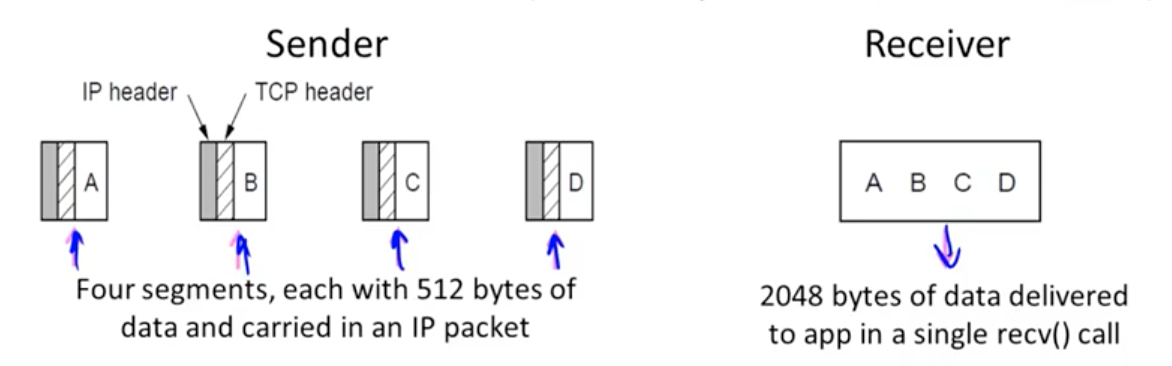
\includegraphics[scale=0.7]{images/6-8-1}
		\caption{ Reliable Bytestream 图一}
		 \label{fig:6-8-1}
		 \end{figure}
		 
		 \item Bidirectional data transfer
		 \begin{itemize}
		 	\item Control information (e.g., ACK) piggybacks(背负着) on data segments in reverse direction
		 	\item 发包并且把上个包的ACK连带着发送过来。
		 \end{itemize}
		 \item See Figure~\ref{fig:6-8-2}
		  
		 \begin{figure}[h!] % h for here.
		\centering
		 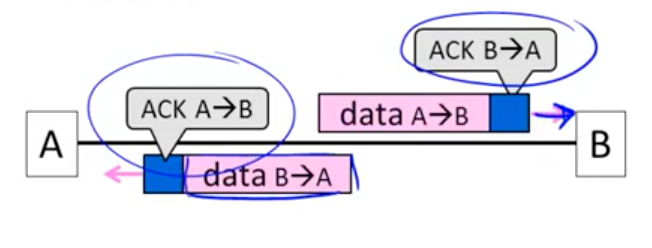
\includegraphics[scale=0.7]{images/6-8-2}
		\caption{ Reliable Bytestream 图二 }
		 \label{fig:6-8-2}
		 \end{figure}
	\end{itemize}
	
	\subsection{TCP Header }
	\begin{itemize}
		\item Ports identify apps (socket API)
		\begin{itemize}
			\item 16-bit identifiers
		\end{itemize}
		
		\item SEQ/ACK used for sliding window
		\begin{itemize}
			\item Selective Repeat, with byte positions
		\end{itemize}
		\item See Figure~\ref{fig:6-8-3}
		  
		 \begin{figure}[h!] % h for here.
		\centering
		 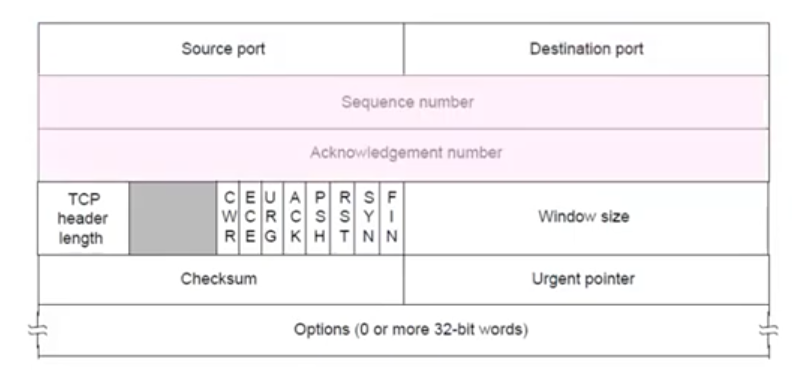
\includegraphics[scale=0.7]{images/6-8-3}
		\caption{ TCP Header }
		 \label{fig:6-8-3}
		 \end{figure}
		 
		 \item SYN/FIN/RST flags for connections
		 \begin{itemize}
		 	\item Flag indicates segment is a SYN etc.
		 \end{itemize}
		 
		 \item Window size for flow control
		 \begin{itemize}
		 	\item Relative to ACK, and in bytes
		 \end{itemize}
		
	\end{itemize}
	
	\subsection{TCP Sliding Window - Receiver}
	\begin{itemize}
		\item \underline{Cumulative ACK} tells next expected byte sequence number ("LAS+1")
		\item Optionally, \underline{selective ACKs} (SACK) give hints for receiver buffer state
		\begin{itemize}
			\item List up to 3 ranges of received bytes
		\end{itemize}
		\item See Figure~\ref{fig:6-8-4}
		  
		 \begin{figure}[h!] % h for here.
		\centering
		 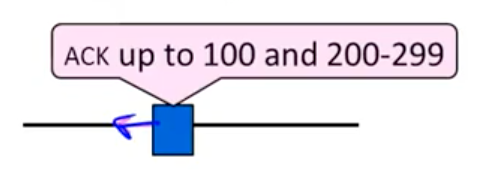
\includegraphics[scale=0.7]{images/6-8-4}
		\caption{ TCP Sliding Window - Receiver }
		 \label{fig:6-8-4}
		 \end{figure}
	\end{itemize}
	
	\subsection{TCP Sliding Window - Sender}
	\begin{itemize}
		\item Uses an adaptive retransmission timeout to resent data from LAS+1
		\item Use heuristics(启发式) to infer loss quickly and resend to avoid timeouts
		\begin{itemize}
			\item "Three duplicate ACKs" treated as loss
		\end{itemize}
		\item See Figure~\ref{fig:6-8-5}
		  
		 \begin{figure}[h!] % h for here.
		\centering
		 \includegraphics[scale=0.7]{images/6-8-5}
		\caption{ TCP Sliding Window - Sender }
		 \label{fig:6-8-5}
		 \end{figure}
		
	\end{itemize}
	
	\subsection{Other TCP Details}
	\begin{itemize}
		\item Many, many quirks(怪癖) you can learn about its operation
		\begin{itemize}
			\item But they are the details
		\end{itemize}
		
		\item Biggest remaining(剩余的) mystery is the workings of congestion(拥塞) control
		\begin{itemize}
			\item We'll tackle this next time!
		\end{itemize}
	\end{itemize}
	
\section{Week 7.1 - Congestion Overview}
	\subsection{Where we are in the Course}
	\begin{itemize}
		\item More fun in the Transport Layer!
		\begin{itemize}
			\item The mystery of congestion control
			\item Depends on the Network layer too
		\end{itemize}
	\end{itemize}
	
	\subsection{Topic of Congestion Overview}
	\begin{itemize}
		\item Understanding congestion, a "traffic jam" in the network
		\begin{itemize}
			\item Later we will learn how to control it
		\end{itemize}
	\end{itemize}
	
	\subsection{Nature of Congestion}
	\begin{itemize}
		\item Routers/switches have internal buffering for contention(争夺)
		\item See Figure~\ref{fig:7-1-1}
		  
		 \begin{figure}[h!] % h for here.
		\centering
		 \includegraphics[scale=0.7]{images/7-1-1}
		\caption{ Nature of Congestion 图一}
		 \label{fig:7-1-1}
		 \end{figure}
		 
		 \item Simplified view of per port output queues
		 \begin{itemize}
		 	\item Typically FIFO (First In First Out), discard when full
		 \end{itemize}
		 \item See Figure~\ref{fig:7-1-2}
		  
		 \begin{figure}[h!] % h for here.
		\centering
		 \includegraphics[scale=0.7]{images/7-1-2}
		\caption{ Nature of Congestion 图二}
		 \label{fig:7-1-2}
		 \end{figure}
		 
		 \item Queues help by absorbing bursts(冲垮) when input > output rate
		 \item But if input > output rate persistently, queue will overflow
		 \begin{itemize}
		 	\item This is congestion
		 \end{itemize}
		 
		 \item Congestion is a function of the traffic patterns - can occur even if every link have the same capacity
	\end{itemize}
	
	\subsection{Effects of Congestion}
	\begin{itemize}
		\item What happens to performance as we increase the load?
		\item See Figure~\ref{fig:7-1-3}
		  
		 \begin{figure}[h!] % h for here.
		\centering
		 \includegraphics[scale=0.7]{images/7-1-3}
		\caption{ Effects of Congestion}
		 \label{fig:7-1-3}
		 \end{figure}
		 
		 \item As offered load rises, congestion occurs as queues begin to fill:
		 \begin{itemize}
		 	\item Delay and loss rise sharply with more load
		 	\item Throughput(吞吐量) falls below load (due to loss)
		 	\item Goodput(有效吞吐量) may fall below throughout (due to spurious(伪) retransmissions)
		 \end{itemize}
		 
		 \item Nore of the above is good!
		 \begin{itemize}
		 	\item Want to operate network just before the onset of congestion
		 \end{itemize}
	\end{itemize}
	
	\subsection{Bandwidth Allocation}
	\begin{itemize}
		\item Important task for network is to allocate its capacity to senders
		\begin{itemize}
			\item Good allocation is efficient and fair
		\end{itemize}
		
		\item \underline{Efficient} means most capacity is used but there is no congestion
		
		\item \underline{Fair} means every sender gets a reasonable share the network
		
		\item Key observation:
		\begin{itemize}
			\item In an effective solution, Transport and Network layers must work together
		\end{itemize}
		
		\item Network layer witnesses(目睹)congestion
		\begin{itemize}
			\item Onlu it can provide direct feedback
		\end{itemize}
		
		\item Transport layer causes congestion
		\begin{itemize}
			\item Only it can reduce offered load
		\end{itemize}
		
		\item Why is it hard? (Just split equally!)
		\begin{itemize}
			\item Number of senders and their offered load is constantly changing
			\item Senders may lack capacity in different parts of the network
			\item Network is distributed; on single party has an overall picture of its state
		\end{itemize}
		
		\item Solution context:
		\begin{itemize}
			\item Senders adapt concurrently based on their own view of the network
			\item Design this adaption so the network usage as a whole is efficient and fair
			\item Adaption is continuous since offered loads continue to change over time
		\end{itemize}
	\end{itemize}
	
	\subsection{Topics}
	\begin{itemize}
		\item {\color{red} 本节课内容:}
		\item Nature of congestion
		
		\item {\color{red} 下节课内容:}
		\item Fair allocations
		\item AIMD control law
		\item TCP Congestion Control history
		\item ACK clocking
		\item TCP Slow-start
		\item TCP Fast Retransmit/Recovery
		\item Congestion Avoidance (ECN)
	\end{itemize}
	
\section{Week 7.2 - Fairness of Allocations}	
	\subsection{Topic of Fairness of Allocations}
	\begin{itemize}
		\item What's a "fair" bandwidth allocation?
		\begin{itemize}
			\item The max-min fair allocation
		\end{itemize}
	\end{itemize}
	
	\subsection{Recall}
	\begin{itemize}
		\item We want a good bandwidth allocation to be fair and efficient
		\begin{itemize}
			\item Now we learn what fair means
		\end{itemize}
		
		\item Caveat(警告): in practice, efficiency is more important than fairness
	\end{itemize}
	
	\subsection{Efficiency vs. Fairness}
	\begin{itemize}
		\item Cannot always have both!
		\begin{itemize}
			\item Example network with traffic $A \rightarrow B$, $B \rightarrow C$ and $A \rightarrow C$
			\item How much traffic can we carry?
		\end{itemize}
		\item See Figure~\ref{fig:7-2-1}
		  
		 \begin{figure}[h!] % h for here.
		\centering
		 \includegraphics[scale=0.7]{images/7-2-1}
		\caption{ Efficiency vs. Fairness 图一}
		 \label{fig:7-2-1}
		 \end{figure}
		 
		 \item If we care about fairness:
		 \begin{itemize}
		 	\item Give equal bandwidth to each flow
		 	\item $A \rightarrow B$: $\frac{1}{2}$ unit, $B \rightarrow C$: $\frac{1}{2}$, and $A \rightarrow C$, $\frac{1}{2}$
		 	\item Total traffic carried is $1 \frac{1}{2}$ units
		 \end{itemize}
		 \item See Figure~\ref{fig:7-2-2}
		  
		 \begin{figure}[h!] % h for here.
		\centering
		 \includegraphics[scale=0.7]{images/7-2-2}
		\caption{ Efficiency vs. Fairness 图二}
		 \label{fig:7-2-2}
		 \end{figure}
		 
		 \item If we care about efficiency:
		 \begin{itemize}
		 	\item Maximize total traffic in network
		 	\item $A \rightarrow B$: 1 unit, $B \rightarrow C$: 1, and $A \rightarrow C$, 0
		 	\item Total traffic rises to 2 units!
		 \end{itemize}
		 \item See Figure~\ref{fig:7-2-3}
		  
		 \begin{figure}[h!] % h for here.
		\centering
		 \includegraphics[scale=0.7]{images/7-2-3}
		\caption{ Efficiency vs. Fairness 图三}
		 \label{fig:7-2-3}
		 \end{figure}
		 
	\end{itemize}
	
	\subsection{The Slippery(光溜溜) Notion of Fairness}
	\begin{itemize}
		\item Why is "equal per flow" fair anyway?
		\begin{itemize}
			\item $A \rightarrow C$ uses more network resources (two links) then $A \rightarrow B$ or $B \rightarrow C$
			\item Host A sends two flows, B sends one
		\end{itemize}
		
		\item Not productive to seek exact fairness
		\begin{itemize}
			\item More important to avoid \underline{starvation}
			\item "Equal per flow" is good enough
		\end{itemize}
	\end{itemize}
	
	\subsection{Generalizing "Equal per Flow"}
	\begin{itemize}
		\item \underline{Bottleneck} for a flow of traffic is the link that limits its bandwidth
		\begin{itemize}
			\item Where congestion occurs for the flow
			\item For $A \rightarrow C$, link A-B is the bottleneck
		\end{itemize}
		\item See Figure~\ref{fig:7-2-4}
		  
		 \begin{figure}[h!] % h for here.
		\centering
		 \includegraphics[scale=0.7]{images/7-2-4}
		\caption{ Generalizing "Equal per Flow" 图一}
		 \label{fig:7-2-4}
		 \end{figure}
		 
		 \item Flows may have different bottlenecks
		 \begin{itemize}
		 	\item For $A \rightarrow B$ link A-B is the bottleneck
		 	\item For $B \rightarrow C$ link B-C is the bottleneck,可能后面网络中有比它更大的容量的线路,此时它就成了瓶颈。
		 	\item Can no longer divide links equally ...
		 \end{itemize}
		 \item See Figure~\ref{fig:7-2-5}
		  
		 \begin{figure}[h!] % h for here.
		\centering
		 \includegraphics[scale=0.7]{images/7-2-5}
		\caption{ Generalizing "Equal per Flow" 图二}
		 \label{fig:7-2-5}
		 \end{figure}
	\end{itemize}
	
	\subsection{Max-Min Fairness}
	\begin{itemize}
		\item Intuitively(直观地), flows bottlenecked on a link get an equal share of that link
		\item \underline{Max-min fair allocation} is one that:
		\begin{itemize}
			\item Increasing the rate of one flow will decrease the rate of a smaller flow
			\item This "maximizes the minimum" flow
		\end{itemize}
		
		\item To find it given a network, imagine "pouring(注入) water into the network"
		\begin{itemize}
			\item {\color{blue} 1.} Start with all flows at rate 0
			\item {\color{blue} 2.} Increase the flows until there is a new bottleneck in the network
			\item {\color{blue} 3.} Hold fixed the rate of the flows that are bottlenecked
			\item {\color{blue} 4.} Go to step 2 for any remaining flows
		\end{itemize}
	\end{itemize}
	
	\subsection{Max-Min Example}
	\begin{itemize}
		\item Example: network with 4 flows, links equal bandwidth
		\begin{itemize}
			\item What is the max-min fair allocation?
		\end{itemize}
		\item See Figure~\ref{fig:7-2-6}
		  
		 \begin{figure}[h!] % h for here.
		\centering
		 \includegraphics[scale=0.7]{images/7-2-6}
		\caption{ Max-Min Example 图一}
		 \label{fig:7-2-6}
		 \end{figure}
		 
		 \item When rate=1/3, flows B,C, and D bottleneck R4-R5
		 \begin{itemize}
		 	\item Fix B, C, and D, continue to increase A
		 \end{itemize}
		 \item See Figure~\ref{fig:7-2-7}
		  
		 \begin{figure}[h!] % h for here.
		\centering
		 \includegraphics[scale=0.7]{images/7-2-7}
		\caption{ Max-Min Example 图二 }
		 \label{fig:7-2-7}
		 \end{figure}
		 
		 \item When $rate = \frac{2}{3}$, flow A bottlenecks R2-R3. Done.
		 \item See Figure~\ref{fig:7-2-8}
		  
		 \begin{figure}[h!] % h for here.
		\centering
		 \includegraphics[scale=0.7]{images/7-2-8}
		\caption{ Max-Min Example 图三 }
		 \label{fig:7-2-8}
		 \end{figure}
		 
		 \item End with A=$\frac{2}{3}$, B, C, D=$\frac{1}{3}$, and R2-R3, R4-R5 full
		 \begin{itemize}
		 	\item Other links have extra capacity that can't be used
		 \end{itemize}
		 \item See Figure~\ref{fig:7-2-9}
		  
		 \begin{figure}[h!] % h for here.
		\centering
		 \includegraphics[scale=0.7]{images/7-2-9}
		\caption{ Max-Min Example 图四 }
		 \label{fig:7-2-9}
		 \end{figure}
		 
	\end{itemize}
	
	\subsection{Adapting over Time}
	\begin{itemize}
		\item Allocation changes as flows start and stop
		 \item See Figure~\ref{fig:7-2-10}
		  
		 \begin{figure}[h!] % h for here.
		\centering
		 \includegraphics[scale=0.7]{images/7-2-10}
		\caption{ Adapting over Time }
		 \label{fig:7-2-10}
		 \end{figure}
	\end{itemize}
	
\section{Week 7.3 - Additive Increase Multiplicative Decrease (AIMD)}
	\subsection{Topic of AIMD}
	\begin{itemize}
		\item Bandwidth allocation models
		\begin{itemize}
			\item Additive Increase Multiplicative Decrease (AIMD) control law
		\end{itemize}
		 \item See Figure~\ref{fig:7-3-1}
		  
		 \begin{figure}[h!] % h for here.
		\centering
		 \includegraphics[scale=0.7]{images/7-3-1}
		\caption{ Topic of AIMD }
		 \label{fig:7-3-1}
		 \end{figure}
	\end{itemize}
	
	\subsection{Recall}
	\begin{itemize}
		\item Want to allocate capacity to senders
		\begin{itemize}
			\item Network layer provides feedback
			\item Transport layer adjusts offered load
			\item A good allocation is efficient and fair
		\end{itemize}
		
		\item How should we perform the allocation?
		\begin{itemize}
			\item Several different possibilities ...
		\end{itemize}
	\end{itemize}
	
	\subsection{Bandwidth Allocation Models}
	\begin{itemize}
		\item Open loop versus closed loop
		\begin{itemize}
			\item Open: reverse bandwidth before use
			\item Closed: use feedback to adjust rates
		\end{itemize}
		
		\item Host versus Network support
		\begin{itemize}
			\item Who is sets/enforces allocations?
		\end{itemize}
		
		\item Window versus Rate based
		\begin{itemize}
			\item How is allocation expressed?
		\end{itemize}
		
		\item {\color{red} TCP is a closed loop, host-driven, and window-based}
		
		\item We'll look at closed-loop, host-driven, and window-based too
		\item Network layer returns feedback on current allocation to senders
		\begin{itemize}
			\item At least tells if there is congestion
		\end{itemize}
		
		\item Transport layer adjusts sender's behavior via window in response
		\begin{itemize}
			\item How senders adapt is a \underline{control law}
		\end{itemize}
	\end{itemize}
	
	\subsection{Additive Increase multiplicative Decrease}
	\begin{itemize}
		\item AIMD is a control low hosts can use to reach a good allocation
		\begin{itemize}
			\item Hosts additively increase rate while network is not congested
			\item Hosts multiplicatively decrease rate when congestion occurs
			\item Used by TCP
		\end{itemize}
		
		\item Let's explore the AIMD game ...
	\end{itemize}
	
	\subsection{AIMD Game}
	\begin{itemize}
		\item Hosts 1 and 2 share a bottleneck
		\begin{itemize}
			\item But do not talk to each other directly
		\end{itemize}
		
		\item Router provides binary feedback
		\begin{itemize}
			\item Tells hosts if network is congested
		\end{itemize}
		\item See Figure~\ref{fig:7-3-2}
		  
		 \begin{figure}[h!] % h for here.
		\centering
		 \includegraphics[scale=0.7]{images/7-3-2}
		\caption{ AIMD Game 图一}
		 \label{fig:7-3-2}
		 \end{figure}
		 
		 \item Each point is a possible allocation
		 \item AI and MD move the allocation
		 \item See Figure~\ref{fig:7-3-3}
		  
		 \begin{figure}[h!] % h for here.
		\centering
		 \includegraphics[scale=0.7]{images/7-3-3}
		\caption{ AIMD Game 图二}
		 \label{fig:7-3-3}
		 \end{figure}
		 
		 \item Play the game !
		 \item Always converge(汇集) to good allocation !
		 \item See Figure~\ref{fig:7-3-4}
		  
		 \begin{figure}[h!] % h for here.
		\centering
		 \includegraphics[scale=0.7]{images/7-3-4}
		\caption{ AIMD Game 图三}
		 \label{fig:7-3-4}
		 \end{figure}
		 
	\end{itemize}
	
	\subsection{AIMD Sawtooth}
	\begin{itemize}
		\item Produces a "sawtooth" pattern over time for rate of each host
		\begin{itemize}
			\item This is the TCP sawtooth (later)
		\end{itemize}
		\item See Figure~\ref{fig:7-3-5}
		  
		 \begin{figure}[h!] % h for here.
		\centering
		 \includegraphics[scale=0.7]{images/7-3-5}
		\caption{ AIMD Sawtooth }
		 \label{fig:7-3-5}
		 \end{figure}
	\end{itemize}
	
	\subsection{AIMD Properties}
	\begin{itemize}
		\item Converges to an allocation that is efficient and fair when hosts run it
		\begin{itemize}
			\item Holds for more general topologies
		\end{itemize}
		
		\item Other increase/decrease control laws do not! (Try MIAD, MIMD, AIAD)
		\item Requires only binary feedback from the network
	\end{itemize}
	
	\subsection{Feedback Signals}
	\begin{itemize}
		\item Several possible signals, with different pros/cons
		\begin{itemize}
			\item We'll look at classic TCP that uses packet loss as a signal
		\end{itemize}
		\item See Figure~\ref{fig:7-3-6}
		  
		 \begin{figure}[h!] % h for here.
		\centering
		 \includegraphics[scale=0.7]{images/7-3-6}
		\caption{ Feedback Signals }
		 \label{fig:7-3-6}
		 \end{figure}
	\end{itemize}
	
\section{Week 7.4 - History of TCP Congestion Control}
	\subsection{Topic of History of TCP Congestion Control}
	\begin{itemize}
		\item The story of TCP congestion control
		\begin{itemize}
			\item Collapse, control, and diversification(多样化)
		\end{itemize}
	\end{itemize}	
	
	\subsection{Congestion Collapse in the 1980s}
	\begin{itemize}
		\item Early TCP used a fixed size sliding window (e.g., 8 packets)
		\begin{itemize}
			\item Initially fine for reliability
		\end{itemize}
		
		\item But something strange happened as the ARPANET grew
		\begin{itemize}
			\item Links stayed busy but transfer rates fell by orders of magnitude(量纲)!
		\end{itemize}
		
		\item Queues became full, retransmissions clogged(堵塞) the network, and \underline{goodput}(有效吞吐量) fell
		\item See Figure~\ref{fig:7-4-1}
		  
		 \begin{figure}[h!] % h for here.
		\centering
		 \includegraphics[scale=0.7]{images/7-4-1}
		\caption{ Congestion Collapse in the 1980s }
		 \label{fig:7-4-1}
		 \end{figure}
	\end{itemize}
	
	\subsection{Van Jacobson (1950-)}
	\begin{itemize}
		\item Widely credited with saving the Internet from congestion collapse in the late 80s
		\begin{itemize}
			\item Introduced congestion control principles
			\item Practical solutions (TCP Tahoe/Reno)
		\end{itemize}
		
		\item Much other pioneering(开拓) work:
		\begin{itemize}
			\item Tools like traceroute, tcpdump, pathchar
			\item IP header compression(压缩), multicast tools
		\end{itemize}
	\end{itemize}
	
	\subsection{TCP Tahoe/Reno}
	\begin{itemize}
		\item Avoid congestion collapse without changing routers (or even receivers)
		\item Idea is to fix timeouts and introduce a \underline{congestion window} (cwnd) over the sliding window to limit queues/loss
		\item TCP Tahoe/Reno implements AIMD by adapting cwnd using packet loss as the network feedback signal
		
		\item TCP behaviors we will study:
		\begin{itemize}
			\item ACK clocking
			\item Adaptive timeout (mean and variance)
			\item Slow-start
			\item Fast Retransmission
			\item Fast Recovery
		\end{itemize}
		
		\item Together, they implement AIMD
	\end{itemize}
	
	\subsection{TCP Timeline}
	\begin{itemize}
		\item See Figure~\ref{fig:7-4-2}
		  
		 \begin{figure}[h!] % h for here.
		\centering
		 \includegraphics[scale=0.7]{images/7-4-2}
		\caption{ TCP Timeline 图一}
		 \label{fig:7-4-2}
		 \end{figure}
		 
		 \item See Figure~\ref{fig:7-4-3}
		  
		 \begin{figure}[h!] % h for here.
		\centering
		 \includegraphics[scale=0.7]{images/7-4-3}
		\caption{ TCP Timeline 图二}
		 \label{fig:7-4-3}
		 \end{figure}
	\end{itemize}
	
\section{Week 7.5 - TCP ACK Clocking}
	\subsection{Topic of TCP ACK Clocking}
	\begin{itemize}
		\item The self-clocking behavior of sliding windows, and how it is used by TCP
		\begin{itemize}
			\item The "ACK clock"
		\end{itemize}
		\item See Figure~\ref{fig:7-5-1}
		  
		 \begin{figure}[h!] % h for here.
		\centering
		 \includegraphics[scale=0.7]{images/7-5-1}
		\caption{ Topic of TCP ACK Clocking}
		 \label{fig:7-5-1}
		 \end{figure}
	\end{itemize}
	
	\subsection{Sliding Window ACK Clock}
	\begin{itemize}
		\item Each in-order ACK advances(促进) the sliding window and  lets a new segment enter the network
		\begin{itemize}
			\item ACKs "clock" data segments
		\end{itemize}
		\item See Figure~\ref{fig:7-5-2}
		  
		 \begin{figure}[h!] % h for here.
		\centering
		 \includegraphics[scale=0.7]{images/7-5-2}
		\caption{ Sliding Window ACK Clock}
		 \label{fig:7-5-2}
		 \end{figure}
	\end{itemize}
	
	\subsection{Benefit of ACK Clocking}
	\begin{itemize}
		\item Consider what happens when sender injects a burst of segments into the network
		\item See Figure~\ref{fig:7-5-3}
		  
		 \begin{figure}[h!] % h for here.
		\centering
		 \includegraphics[scale=0.7]{images/7-5-3}
		\caption{ Benefit of ACK Clocking}
		 \label{fig:7-5-3}
		 \end{figure}
		 
		 \item Segments are buffered and spread out on slow link
		 \item See Figure~\ref{fig:7-5-4}
		  
		 \begin{figure}[h!] % h for here.
		\centering
		 \includegraphics[scale=0.7]{images/7-5-4}
		\caption{ Benefit of ACK Clocking}
		 \label{fig:7-5-4}
		 \end{figure}
		 
		 \item ACKs maintain the spread back to the original sender
		 \item See Figure~\ref{fig:7-5-5}
		  
		 \begin{figure}[h!] % h for here.
		\centering
		 \includegraphics[scale=0.7]{images/7-5-5}
		\caption{ Benefit of ACK Clocking}
		 \label{fig:7-5-5}
		 \end{figure}
		 
		 \item Sender clocks new segments with the spread
		 \begin{itemize}
		 	\item Now sending at the bottleneck link without queuing!
		 \end{itemize}
		  \item See Figure~\ref{fig:7-5-6}
		  
		 \begin{figure}[h!] % h for here.
		\centering
		 \includegraphics[scale=0.7]{images/7-5-6}
		\caption{ Benefit of ACK Clocking}
		 \label{fig:7-5-6}
		 \end{figure}		 
		 
		 \item Helps the network run with low levels of loss and delay
		 \item The network has smoothed out the burst of data segments
		 \item ACK clock transfers this smooth timing back to the sender
		 \item Subsequent data segments are not sent in bursts so do not queue up in the network
	\end{itemize}
	
	\subsection{TCP Uses ACK Clocking}
	\begin{itemize}
		\item TCP uses a sliding window because of the value of ACK clocking
		
		\item Sliding window controls how many segments are inside the network
		\begin{itemize}
			\item Called the \underline{congestion window}, or \underline{cwnd}
			\item Rate is roughly cwnd/RTT 
		\end{itemize}
		
		\item TCP only sends small bursts of segments to let the network keep the traffic smooth
	\end{itemize}
	
\section{Week 7.6 - TCP Slow Start}
	\subsection{Topic of TCP Slow Start}
	\begin{itemize}
		\item How TCP implements AIMD, part 1
		\begin{itemize}
			\item "Slow start" is a component of the AI portion of AIMD
		\end{itemize}
		\item See Figure~\ref{fig:7-6-1}
		  
		 \begin{figure}[h!] % h for here.
		\centering
		 \includegraphics[scale=0.7]{images/7-6-1}
		\caption{ Topic of TCP Slow Start}
		 \label{fig:7-6-1}
		 \end{figure}	
	\end{itemize}
	
	\subsection{Recall}
	\begin{itemize}
		\item We want TCP to follow an AIMD control low for a good allocation
		\item Sender uses a \underline{congestion window} or \underline{cwnd} to set its rate ($\approx cwnd / RTT$)
		\item Sender uses packet loss as the network congestion signal
		\item Need TCP to work across a very large range of rates and RTTs
	\end{itemize}
	
	\subsection{TCP Startup Problem}
	\begin{itemize}
		\item We want to quickly near the right rate, $cwnd_{IDEAL}$, but it varies greatly
		\begin{itemize}
			\item Fixed sliding window doesn't adapt and is rough on the network (loss!)
			\item AI with small bursts adapts cwnd gently to the network, but might take a long time to become efficient
		\end{itemize}
	\end{itemize}
	
	\subsection{Slow-Start Solution}
	\begin{itemize}
		\item Start by doubling cwnd every RTT
		\begin{itemize}
			\item Exponential grownth (1, 2, 4, 8, 16, ...)
			\item Start slow, quickly reach large values
		\end{itemize}
		\item See Figure~\ref{fig:7-6-2}
		  
		 \begin{figure}[h!] % h for here.
		\centering
		 \includegraphics[scale=0.7]{images/7-6-2}
		\caption{ Slow-Start Solution 图一 }
		 \label{fig:7-6-2}
		 \end{figure}	
		 
		 \item Eventually packet loss will occur when the network is congested
		 \begin{itemize}
		 	\item Loss timeout tells us cwnd is too large
		 	\item Next time, switch to AI beforehand(预先)
		 	\item Slowly adapt cwnd near right value
		 \end{itemize}
		 
		 \item In terms of cwnd:
		 \begin{itemize}
		 	\item Expect loss for $ cwnd_{C} \thickapprox 2BD + queue $
		 	\item Use $ssthresh = cwnd_{C}/2 $ to switch to AI
		 \end{itemize}
		 
		 \item Combined behavior, after first time
		 \begin{itemize}
		 	\item Most time spend near right value
		 \end{itemize}
		 \item See Figure~\ref{fig:7-6-3}
		  
		 \begin{figure}[h!] % h for here.
		\centering
		 \includegraphics[scale=0.7]{images/7-6-3}
		\caption{ Slow-Start Solution 图二 }
		 \label{fig:7-6-3}
		 \end{figure}	
	\end{itemize}
	
	\subsection{Slow-Start (Doubling) Timeline}
	\begin{itemize}
		\item 左侧的cwnd是一个一个地增加的
		\item See Figure~\ref{fig:7-6-4}
		  
		 \begin{figure}[h!] % h for here.
		\centering
		 \includegraphics[scale=0.7]{images/7-6-4}
		\caption{ Slow-Start (Doubling) Timeline }
		 \label{fig:7-6-4}
		 \end{figure}
	\end{itemize}
	
	\subsection{Additive Increase Timeline}
	\begin{itemize}
		\item 和上面那副图一样,左边的cwnd是一个一个地增加,这里增加的速度比上面慢多了。
		\item See Figure~\ref{fig:7-6-5}
		  
		 \begin{figure}[h!] % h for here.
		\centering
		 \includegraphics[scale=0.7]{images/7-6-5}
		\caption{ Additive Increase Timeline }
		 \label{fig:7-6-5}
		 \end{figure}
	\end{itemize}
	
	\subsection{TCP Tahoe (Implementation)}
	\begin{itemize}
		\item Initial slow-start (doubling) phase
		\begin{itemize}
			\item Start with $cwnd = 1$ (or small value)
			\item $cwnd +=1$ packet per ACK
		\end{itemize}
		
		\item Later Additive Increase phase
		\begin{itemize}
			\item $ cwnd += 1/cwnd$ packets per ACK
			\item Roughly adds 1 packet per RTT
		\end{itemize}
		
		\item Switching threshold (initially infinity)
		\begin{itemize}
			\item Switch to AI when $ cwnd > ssthread $
			\item Set $ ssthresh = cwnd/2 $ after loss
			\item Begin with slow-start after timeout
		\end{itemize}
	\end{itemize}
	
	\subsection{Timeout Misfortunes(不幸)}
	\begin{itemize}
		\item Why do a slow-start after timeout?
		\begin{itemize}
			\item Instead of MD cwnd (for AIMD)
		\end{itemize}
		
		\item Timeouts are sufficiently long that the ACK clock will have run down(撞倒)
		\begin{itemize}
			\item Slow-start ramps(上坡) up the ACK clock
		\end{itemize}
		
		\item We need to detect loss before a timeout to get to full AIMD
		\begin{itemize}
			\item Done in TCP Reno (next time)
		\end{itemize}
	\end{itemize}
	
\section{Week 7.7 - TCP Fast Retransmit : Fast Recovery}	
	\subsection{Topic of TCP Fast Retransmit : Fast Recovery }
	\begin{itemize}
		\item How TCP implements AIMD, part 2
		\begin{itemize}
			\item "Fast retransmit" and "fast recovery" are the MD portion of AIMD
		\end{itemize}
		\item See Figure~\ref{fig:7-7-1}
		  
		 \begin{figure}[h!] % h for here.
		\centering
		 \includegraphics[scale=0.7]{images/7-7-1}
		\caption{ Topic of TCP Fast Retransmit : Fast Recovery }
		 \label{fig:7-7-1}
		 \end{figure}
	\end{itemize}
	
	\subsection{Recall}
	\begin{itemize}
		\item We want TCP to follow an AIMD control law for a good allocation
		\item Sender uses a \underline{congestion window} or \underline{cwnd} to set its rate ($\approx cwnd/RTT$)
		\item Sender uses slow-start to ramp up(斜坡上升) the ACK clock, followed by Additive Increase
		\item But after a timeout, sender slow-starts again with cwnd=1 (as it no ACK clock)
	\end{itemize}
	
	\subsection{Inferring(推斷) Loss from ACKs}
	\begin{itemize}
		\item TCP uses a cumulative ACK
		\begin{itemize}
			\item Carries highest in-order seq. number
			\item Normally a steady advance
		\end{itemize}
		
		\item Duplicate ACKs give us hints about what data hasn't arrived
		\begin{itemize}
			\item Tell us some new data did arrive, but it was not next segment
			\item Thus the next segment may be lost
		\end{itemize}
	\end{itemize}
	
	\subsection{Fast Retransmit}
	\begin{itemize}
		\item Treat three duplicate ACKs as a loss
		\begin{itemize}
			\item Retransmit next expected segment
			\item Some repetition allows for reordering, but still detects loss quickly
		\end{itemize}
		\item See Figure~\ref{fig:7-7-2}
		  
		 \begin{figure}[h!] % h for here.
		\centering
		 \includegraphics[scale=0.7]{images/7-7-2}
		\caption{ Fast Retransmit 图一}
		 \label{fig:7-7-2}
		 \end{figure}
		 \item See Figure~\ref{fig:7-7-3}
		  
		 \begin{figure}[h!] % h for here.
		\centering
		 \includegraphics[scale=0.7]{images/7-7-3}
		\caption{ Fast Retransmit 图二 }
		 \label{fig:7-7-3}
		 \end{figure}
		 
		 \item It can repair single segment loss quickly, typically before a timeout
		\item However, we have quiet time at the sender/receiver while waiting for the ACK to jump
		\item And we still need to MD cwnd ...	 
	\end{itemize}
	
	\subsection{Inferring(推斷) Non-Loss from ACKs}
	\begin{itemize}
		\item Duplicate ACKs also give us hints about what data has arrived
		\begin{itemize}
			\item Each new duplicate ACK means that some new segment has arrived
			\item It will be the segments after the loss
			\item Thus advancing the sliding window will not increase the number of segments stored in the network
		\end{itemize}
	\end{itemize}
	
	\subsection{Fast Recovery}
	\begin{itemize}
		\item First fast retransmit, and MD cwnd
		\item Then pretend further duplicate ACKs are the expected ACKs
		\begin{itemize}
			\item Lets new segments be sent for ACKs
			\item Reconcile(調和) views when the ACK jumps
		\end{itemize}
		\item See Figure~\ref{fig:7-7-4}
		  
		 \begin{figure}[h!] % h for here.
		\centering
		 \includegraphics[scale=0.7]{images/7-7-4}
		\caption{ Fast Recovery 图一 }
		 \label{fig:7-7-4}
		 \end{figure}
		 
		 \item 如下图所示,把最后的Ack 13当成Ack 20 可以让Sender和 Receiver不用等待,持续发送与接收包。
		 \item See Figure~\ref{fig:7-7-5}
		  
		 \begin{figure}[h!] % h for here.
		\centering
		 \includegraphics[scale=0.7]{images/7-7-5}
		\caption{ Fast Recovery 图二 }
		 \label{fig:7-7-5}
		 \end{figure}
		 
		 \item With fast retransmit, it repairs a single segment loss quickly and keeps the ACK clock running
		 
		 \item This allows us to realize AI<D
		 \begin{itemize}
		 	\item No timeouts or slow-start after loss, just continue with a smaller cwnd
		 \end{itemize}
		 
		 \item TCP Reno combines slow-start, fast retransmit and fast recovery
		 \begin{itemize}
		 	\item Multiplicative Decrease is $\frac{1}{2}$
		 \end{itemize}
		 \item See Figure~\ref{fig:7-7-6}
		  
		 \begin{figure}[h!] % h for here.
		\centering
		 \includegraphics[scale=0.7]{images/7-7-6}
		\caption{ Fast Recovery 图三 }
		 \label{fig:7-7-6}
		 \end{figure}
	\end{itemize}
	
	\subsection{TCP Reno, NewReno, and SACK}
	\begin{itemize}
		\item Reno can repair one loss per RTT
		\begin{itemize}
			\item Multiple losses cause a timeout
		\end{itemize}
		
		\item NewReno further refines(提煉) ACK heuristics(試探)
		\begin{itemize}
			\item Repairs multiple losses without timeout
		\end{itemize}
		
		\item SACK is a better idea
		\begin{itemize}
			\item Receiver sends ACK ranges so sender can retransmit without guesswork
		\end{itemize}
	\end{itemize}
	
\section{Week 7.8 - Explicit Congestion Notification (ECN)}
	\subsection{Topic of ECN}
	\begin{itemize}
		\item How routers can help hosts to avoid congestion
		\begin{itemize}
			\item Explicit Congestion Notification
		\end{itemize}
		\item See Figure~\ref{fig:7-8-1}
		  
		 \begin{figure}[h!] % h for here.
		\centering
		 \includegraphics[scale=0.7]{images/7-8-1}
		\caption{ Topic of ECN }
		 \label{fig:7-8-1}
		 \end{figure}
	\end{itemize}
	
	\subsection{Congestion Avoidance vs. Control}
	\begin{itemize}
		\item Classic TCP drives the network into congestion and then recovers
		\begin{itemize}
			\item Needs to see to slow down
		\end{itemize}
		
		\item Would be better to use the network but avoid congestion altogether(完全) !
		\begin{itemize}
			\item Reduces loss and delay
		\end{itemize}
		
		\item But how can we do this ?
	\end{itemize}
	
	\subsection{Feedback Signals}
	\begin{itemize}
		\item Delay and router signals can let us avoid congestion
		\item See Figure~\ref{fig:7-8-2}
		  
		 \begin{figure}[h!] % h for here.
		\centering
		 \includegraphics[scale=0.7]{images/7-8-2}
		\caption{ Feedback Signals }
		 \label{fig:7-8-2}
		 \end{figure}
	\end{itemize}
	
	\subsection{ECN (Explicit Congestion Notification)}
	\begin{itemize}
		\item Router detects the onset(發作) of congestion via its queue
		\begin{itemize}
			\item When congested, it \underline{marks} affected packets (IP header)
		\end{itemize}
		\item See Figure~\ref{fig:7-8-3}
		  
		 \begin{figure}[h!] % h for here.
		\centering
		 \includegraphics[scale=0.7]{images/7-8-3}
		\caption{ ECN (Explicit Congestion Notification) }
		 \label{fig:7-8-3}
		 \end{figure}
		 
		 \item Marked packets arrive at receiver; treated as loss
		 \begin{itemize}
		 	\item TCP receiver reliably informs(告知) TCP sender of the congestion
		 \end{itemize}
		 
		 \item Advantages:
		 \begin{itemize}
		 	\item Routers deliver clear signal to hosts
		 	\item Congestion is detected early, no loss
		 	\item No extra packets need to be sent
		 \end{itemize}
		 
		 \item Disadvantages:
		 \begin{itemize}
		 	\item Routers and hosts must be upgraded
		 \end{itemize}
	\end{itemize}
	
	
\section{Week 8.1 - Application Layer Overview}
	\subsection{Where we are in the Course}
	\begin{itemize}
		\item Starting the Application Layer!
		\begin{itemize}
			\item Builds distributed "network services" (DNS, Web) on Transport services
		\end{itemize}
	\end{itemize}
	
	\subsection{Recall}
	\begin{itemize}
		\item Application layer protocols are often part of an "app"
		\begin{itemize}
			\item But don't need a GUI, e.g., DNS
		\end{itemize}
		\item See Figure~\ref{fig:8-1-1}
		  
		 \begin{figure}[h!] % h for here.
		\centering
		 \includegraphics[scale=0.7]{images/8-1-1}
		\caption{ Recall 图一}
		 \label{fig:8-1-1}
		 \end{figure}
		 
		 \item Application layer messages are often split over multiple packets
		 \begin{itemize}
		 	\item Or may be aggregated(集成體) in packet ...
		 \end{itemize}
		 \item See Figure~\ref{fig:8-1-2}
		  
		 \begin{figure}[h!] % h for here.
		\centering
		 \includegraphics[scale=0.7]{images/8-1-2}
		\caption{ Recall 图二 }
		 \label{fig:8-1-2}
		 \end{figure}
	\end{itemize}
	
	\subsection{Application Communication Needs}
	\begin{itemize}
		\item Vary widely with app; must build on Transport services
		\item See Figure~\ref{fig:8-1-3}
		  
		 \begin{figure}[h!] % h for here.
		\centering
		 \includegraphics[scale=0.7]{images/8-1-3}
		\caption{ Application Communication Needs }
		 \label{fig:8-1-3}
		 \end{figure}
	\end{itemize}
	
	\subsection{OSI Session/Presentation Layers}
	\begin{itemize}
		\item Remember this? Two relevant concepts ...
		\item See Figure~\ref{fig:8-1-4}
		  
		 \begin{figure}[h!] % h for here.
		\centering
		 \includegraphics[scale=0.7]{images/8-1-4}
		\caption{ OSI Session/Presentation Layers }
		 \label{fig:8-1-4}
		 \end{figure}
	\end{itemize}
	
	\subsection{Session Concept}
	\begin{itemize}
		\item A session is a series of related network interactions in support of an application task
		\begin{itemize}
			\item Often informal, not explicit
		\end{itemize}
		
		\item Examples:
		\begin{itemize}
			\item Web page fetches multiple resources
			\item Skype call involves audio, video, chat
		\end{itemize}
	\end{itemize}
	
	\subsection{Presentation Concept}
	\begin{itemize}
		\item Apps need to identify the type of content, and encode it for transfer
		\begin{itemize}
			\item These are Presentation functions
		\end{itemize}
		
		\item Examples:
		\begin{itemize}
			\item Media (MIME) types, e.g., image/jpeg, identify the type of content
			\item Transfer encodings, e.g., gzip, identify the encoding of the content
			\item Application headers are often simple and readable versus packed for efficiency
		\end{itemize}
	\end{itemize}
	
	\subsection{Evolution(演化) of Internet Application}
	\begin{itemize}
		\item Always changing, and growing ...
		\item See Figure~\ref{fig:8-1-5}
		  
		 \begin{figure}[h!] % h for here.
		\centering
		 \includegraphics[scale=0.7]{images/8-1-5}
		\caption{ Evolution(演化) of Internet Application}
		 \label{fig:8-1-5}
		 \end{figure}
		 
		 \item For a peek(窺視) at the state of the Internet:
		 \begin{itemize}
		 	\item Akamai's State of the Internet Report (quarterly(每季度的))
		 	\item Cisco's Visual Networking Index
		 	\item Mary Meeker's Internet Report
		 \end{itemize}
		 
		 \item Robust Internet growth, esp. video, wireless and mobile
		 \begin{itemize}
		 	\item Most traffic is video, will be 90\% of Internet in a few years
		 	\item Wireless traffic will soon overtake wired traffic
		 	\item Mobile traffic is still a small portion (15\%) of overall
		 	\item Growing attack traffic from China, also U.S. and Russia
		 \end{itemize}
	\end{itemize}
	
	\subsection{Topics}
	\begin{itemize}
		\item {\color{red} 本次所讲的内容}
		\item Evolving Internet applications
		
		\item {\color{red} 下次要讲的内容}
		\item DNS (Domain Name System)
		\item HTTP (HyperText Transfer Protocol)
		\item Web proxies(代理人) and caching
		\item Content Distribution Networks
		\item Peer-to-peer (BitTorrent)
		
		\item {\color{red} 再晚一些要讲的内容}
		\item Real-time applications (VoIP)
	\end{itemize}
	
\section{Week 8.2 - DNS Part 1}	
	\subsection{Topic of DNS Part 1}
	\begin{itemize}
		\item The DNS (Domain Name System)
		\begin{itemize}
			\item Human-readable host names, and more
			\item Part 1: the distributed namespace
		\end{itemize}
		\item See Figure~\ref{fig:8-2-1}
		  
		 \begin{figure}[h!] % h for here.
		\centering
		 \includegraphics[scale=0.7]{images/8-2-1}
		\caption{ Topic of DNS Part 1 }
		 \label{fig:8-2-1}
		 \end{figure}
	\end{itemize}
	
	\subsection{Names and Addresses}
	\begin{itemize}
		\item \underline{Names} are higher-level identifiers for resources
		\item \underline{Addresses} are lower-level locators for resources
		\begin{itemize}
			\item Multiple levels, e.g. full name $\rightarrow$ email $\rightarrow$ IP address $\rightarrow$ Ethernet address
		\end{itemize}
		
		\item \underline{Resolution(解析)} (or lookup) is mapping a name to an address
		\item See Figure~\ref{fig:8-2-2}
		  
		 \begin{figure}[h!] % h for here.
		\centering
		 \includegraphics[scale=0.7]{images/8-2-2}
		\caption{ Names and Addresses }
		 \label{fig:8-2-2}
		 \end{figure}
	\end{itemize}
	
	\subsection{Before the DNS - HOSTS.TXT}
	\begin{itemize}
		\item Directory was a file HOSTS.TXT regularly retrieved(取回) for all hosts from a central machine at the NIC (Network Information Center)
		\item Names were initially flat, became hierarchical (e.g., lcs.mit.edu) ~85
		\item Neither manageable nor efficient as the ARPANET grew ...
	\end{itemize}
	
	\subsection{DNS}
	\begin{itemize}
		\item A naming service to map between host names and their IP addresses (and more)
		\begin{itemize}
			\item www.uwa.edu.au $\rightarrow$ 130.95.128.140
		\end{itemize}
		
		\item Goals:
		\begin{itemize}
			\item Easy to manage (esp. with multiple parties)
			\item Efficient (good performance, few resources)
		\end{itemize}
		
		\item Approach:
		\begin{itemize}
			\item Distributed directory based on a hierarchical namespace
			\item Automated(使自動化) protocol to tie pieces together
		\end{itemize}
	\end{itemize}
	 
	 
	 \subsection{DNS Namespace}
	 \begin{itemize}
	 	\item Hierarchical, starting from "." (dot, typically omitted)
	 	\item See Figure~\ref{fig:8-2-3}
		  
		 \begin{figure}[h!] % h for here.
		\centering
		 \includegraphics[scale=0.7]{images/8-2-3}
		\caption{ DNS Namespace }
		 \label{fig:8-2-3}
		 \end{figure}
	 \end{itemize}
	 
	 \subsection{TLDs (Top-Level Domains)}
	 \begin{itemize}
	 	\item Run by ICANN (Internet Corp. for Assigned Names and Numbers)
	 	\begin{itemize}
	 		\item Starting in 1998; naming is financial, political, and international
	 	\end{itemize}
	 	
	 	\item 22+ generic TLDs
	 	\begin{itemize}
	 		\item Initially .com, .edu, .gov, .mil, .org, .net
	 		\item Added .aero, .museum, etc. from 2001 through .xxx in 2011
	 		\item Different TLDs have different usage policies(有些可以乱用,但是如edu则是虚教育机构才可以)
	 	\end{itemize}
	 	
	 	\item ~250 country code TLDs
	 	\begin{itemize}
	 		\item Two letters, e.g., ".au", plus international characters(比如汉字) since 2010
	 		\item Widely commercialized, e.g., .tv (Tuvalu)
	 		\item Many domain hacks, e.g., instagr.am (Armenia), goo.gl (Greenland)
	 	\end{itemize}
	 \end{itemize}
	 
	 \subsection{DNS Zones}
	 \begin{itemize}
	 	\item A \underline{zone} is a contiguous(毗鄰的) portion of the namespace
	 	\item See Figure~\ref{fig:8-2-4}
		  
		 \begin{figure}[h!] % h for here.
		\centering
		 \includegraphics[scale=0.7]{images/8-2-4}
		\caption{ DNS Zones}
		 \label{fig:8-2-4}
		 \end{figure}
	 	 
		 \item Zones are the basis for distribution
		 \begin{itemize}
		 	\item EDU Registrar administers .edu
		 	\item UW administers washington.edu
		 	\item CS\&E administers cs.washington.edu
		 \end{itemize}
		 
		 \item Each zone has a nameserver to contact(聯繫) for information about it
		 \begin{itemize}
		 	\item Zone must include contacts for delegations(分配;委派), e.g., .edu knows nameserver for washington.edu
		 	\item 也就是每个域至少需要一台nameserver来接收上一层所发来的信息,并回复下一层的信息到上一层。做的是桥梁的作用,把子域的孤岛信息由这个桥梁连接到上一层的码头上。
		 \end{itemize}
	 \end{itemize}
	 
	 \subsection{DNS Resource Records}
	 \begin{itemize}
	 	\item A zone is comprised(組成) of DNS resource records that give information for its domain names
	 	\item See Figure~\ref{fig:8-2-5}
		  
		 \begin{figure}[h!] % h for here.
		\centering
		 \includegraphics[scale=0.7]{images/8-2-5}
		\caption{ DNS Resource Records 图一 }
		 \label{fig:8-2-5}
		 \end{figure}
		 
		 \item 下面是一个DNS资源记录的例子
		 \item See Figure~\ref{fig:8-2-6}
		  
		 \begin{figure}[h!] % h for here.
		\centering
		 \includegraphics[scale=0.7]{images/8-2-6}
		\caption{ DNS Resource Records 图二 }
		 \label{fig:8-2-6}
		 \end{figure}
	 \end{itemize}
	
\section{Week 8.3 - DNS Part 2}
	\subsection{Topic of DNS Part 2 }
	\begin{itemize}
		\item Human-readable host names, and more
		\item Part2: Name resolution
	\end{itemize}
	
	\subsection{Recall}
	\begin{itemize}
		\item A \underline{zone} is a contiguous portion of the namespace
		\begin{itemize}
			\item Each zone is managed by one or more \underline{nameservers}
		\end{itemize}
		\item See Figure~\ref{fig:8-3-1}
		  
		 \begin{figure}[h!] % h for here.
		\centering
		 \includegraphics[scale=0.7]{images/8-3-1}
		\caption{ Recall }
		 \label{fig:8-3-1}
		 \end{figure}
	\end{itemize}
	
	\subsection{DNS Resolution(解析)}
	\begin{itemize}
		\item DNS protocol lets a host resolve any host name (domain) to IP address
		\item If unknown, can start with the root nameserver and work down zones
		\item Let's see an example first ...
		
		\item flits.cs.vu.nl resolves robot.cs.washington.edu
		\item See Figure~\ref{fig:8-3-2}
		  
		 \begin{figure}[h!] % h for here.
		\centering
		 \includegraphics[scale=0.7]{images/8-3-2}
		\caption{ DNS Resolution(解析) }
		 \label{fig:8-3-2}
		 \end{figure}
	\end{itemize}
	
	\subsection{Iterative vs. Recursive Queries}
	\begin{itemize}
		\item Recursive query
		\begin{itemize}
			\item Nameserver completes resolution and returns the final answer
			\item E.g., flits(輕快地飛(或移動)) $\rightarrow$ local nameserver
			
			\item Lets server offload(卸去(累贅)) client burden(負荷) (simple resolvers) for manageability
			\item Lets server cache over a pool of clients for better performance
		\end{itemize}
		
		\item Iterative query
		\begin{itemize}
			\item Nameserver returns the answer or who to contact next for the answer
			\item E.g., local nameserver $\rightarrow$ all others
			
			\item Lets server "file and forget"
			\item Easy to build high load servers
		\end{itemize}
	\end{itemize}
	
	\subsection{Caching}
	\begin{itemize}
		\item Resolution latency should be low
		\begin{itemize}
			\item adds delay to web browsing ,教授没说明原因。
		\end{itemize}
		
		\item Cache query/responses to answer future queries immediately
		\begin{itemize}
			\item Including partial (iterative) answers
			\item Responses carry a TTL for caching ,一般TTL设置为1天吧
		\end{itemize}
		\item See Figure~\ref{fig:8-3-3}
		  
		 \begin{figure}[h!] % h for here.
		\centering
		 \includegraphics[scale=0.7]{images/8-3-3}
		\caption{ Caching  图一}
		 \label{fig:8-3-3}
		 \end{figure}
		 
		 \item flits.cs.vu.nl resolves eng.washington.edu
		 \begin{itemize}
		 	\item And previous resolutions cut out most of the process
		 \end{itemize}
		 \item See Figure~\ref{fig:8-3-4}
		  
		 \begin{figure}[h!] % h for here.
		\centering
		 \includegraphics[scale=0.7]{images/8-3-4}
		\caption{ Caching  图二}
		 \label{fig:8-3-4}
		 \end{figure}
		 
	\end{itemize}
	
	\subsection{Local Nameservers}
	\begin{itemize}
		\item Local nameservers typically run by IT (enterprise, ISP)
		\begin{itemize}
			\item But may be your host or AP
			\item Or alternatives e.g., Google public DNS
		\end{itemize}
		
		\item Clients need to be able to contact their local nameservers
		\begin{itemize}
			\item Typically configured via DHCP
		\end{itemize}
	\end{itemize}
	
	\subsection{Root Nameservers}
	\begin{itemize}
		\item Root (dot) is served by 13 server names
		\begin{itemize}
			\item a.root-servers.net to m.root-servers.net
			\item All nameservers need root IP addresses
			\item Handled via configuration file (named.ca)
		\end{itemize}
		
		\item There are $>250$ distributed server instances
		\begin{itemize}
			\item Highly reachable, reliable service
			\item Most servers are reached by \underline{IP anycast(任播是与单播(unicast)、广播(broadcast)和多播(multicast)不同的方式)} (Multiple locations advertise same IP ! Routes take client to the closest one. See §5.2.9)
			\item Servers are IPv4 and IPv6 reachable
		\end{itemize}
	\end{itemize}
	
	\subsection{DNS Protocol}
	\begin{itemize}
		\item Query and response messages
		\begin{itemize}
			\item Built on UDP messages, port 53
			\item ARQ for reliability; server is stateless!
			\item Messages linked by a 16-bit ID field
		\end{itemize}
		\item See Figure~\ref{fig:8-3-5}
		  
		 \begin{figure}[h!] % h for here.
		\centering
		 \includegraphics[scale=0.7]{images/8-3-5}
		\caption{ DNS Protocol  图一}
		 \label{fig:8-3-5}
		 \end{figure}
		 
		 \item Service reliability via replicas
		 \begin{itemize}
		 	\item Run multiple nameservers for domain
		 	\item Return the list; clients use one answer
		 	\item Helps distribute load too
		 \end{itemize}
		 \item See Figure~\ref{fig:8-3-6}
		  
		 \begin{figure}[h!] % h for here.
		\centering
		 \includegraphics[scale=0.7]{images/8-3-6}
		\caption{ DNS Protocol 图二 }
		 \label{fig:8-3-6}
		 \end{figure}
		 
		 \item Security is a major issue
		 \begin{itemize}
		 	\item Compromise(損害) redirects to wrong site!
		 	\item Not part of initial protocols ...
		 \end{itemize}
		 
		 \item DNSSEC (DNS Security Extensions)
		 \begin{itemize}
		 	\item Long under development, now partially deployed. We'll look at it later
		 \end{itemize}
	\end{itemize}
	
\section{Week 8.4 - HTTP Introduction}
	\subsection{Topic of HTTP Introduction}
	\begin{itemize}
		\item HTTP, (HyperText Transfer Protocol)
		\begin{itemize}
			\item Basis for fetching Web pages
		\end{itemize}
		\item See Figure~\ref{fig:8-4-1}
		  
		 \begin{figure}[h!] % h for here.
		\centering
		 \includegraphics[scale=0.7]{images/8-4-1}
		\caption{ Topic of HTTP Introduction }
		 \label{fig:8-4-1}
		 \end{figure}
	\end{itemize}
	
	\subsection{Sir Tim Berners-Lee (1955-)}
	\begin{itemize}
		\item Inventor of the Web
		\begin{itemize}
			\item Dominant(主要的) Internet app since mid 90s
			\item He now directs the W3C
		\end{itemize}
		
		\item Developed Web at CERN in 1989
		\begin{itemize}
			\item Browser, server and first HTTP
			\item Popularized via Mosaic (1993), Netscape
			\item First WWW conference in 1994
		\end{itemize}
	\end{itemize}
	
	\subsection{Web Context}
	\begin{itemize}
		\item See Figure~\ref{fig:8-4-2}
		  
		 \begin{figure}[h!] % h for here.
		\centering
		 \includegraphics[scale=0.7]{images/8-4-2}
		\caption{ Web Context }
		 \label{fig:8-4-2}
		 \end{figure}
	\end{itemize}
	
	\subsection{HTTP Context}
	\begin{itemize}
		\item HTTP is a request/response protocol for fetching Web resources
		\begin{itemize}
			\item Runs on TCP, typically port 80
			\item Part of browser/server app
		\end{itemize}
		\item See Figure~\ref{fig:8-4-3}
		  
		 \begin{figure}[h!] % h for here.
		\centering
		 \includegraphics[scale=0.7]{images/8-4-3}
		\caption{ HTTP Context }
		 \label{fig:8-4-3}
		 \end{figure}
	\end{itemize}
	
	\subsection{Fetching a Web page with HTTP}
	\begin{itemize}
		\item Start with the page URL:
		\item See Figure~\ref{fig:8-4-4}
		  
		 \begin{figure}[h!] % h for here.
		\centering
		 \includegraphics[scale=0.7]{images/8-4-4}
		\caption{ Fetching a Web page with HTTP }
		 \label{fig:8-4-4}
		 \end{figure}
		 
		 \item Steps:
		 \begin{itemize}
		 	\item Resolve the server to IP address (DNS)
		 	\item Set up TCP connection to the server
		 	\item Send HTTP request for the page
		 	\item (Await HTTP response for the page)
		 	\item {\color{pink} **} Execute / fetch embedded resources / render(绘制)
		 	\item Clean up any idle TCP connections
		 \end{itemize}
	\end{itemize}
	
	\subsection{Static vs Dynamic Web pages}
	\begin{itemize}
		\item Static web page is a file contents, e.g., image
		\item Dynamic web page is the result of program execution
		\begin{itemize}
			\item Javascript on client, PHP on server, or both
		\end{itemize}
		\item See Figure~\ref{fig:8-4-5}
		  
		 \begin{figure}[h!] % h for here.
		\centering
		 \includegraphics[scale=0.7]{images/8-4-5}
		\caption{ Static vs Dynamic Web pages}
		 \label{fig:8-4-5}
		 \end{figure}
	\end{itemize}
	
	\subsection{Evolution of HTTP}
	\begin{itemize}
		\item Consider security (SSL/TLS for HTTPS) later
		\item See Figure~\ref{fig:8-4-6}
		  
		 \begin{figure}[h!] % h for here.
		\centering
		 \includegraphics[scale=0.7]{images/8-4-6}
		\caption{ Evolution of HTTP }
		 \label{fig:8-4-6}
		 \end{figure}
	\end{itemize}
	
	\subsection{HTTP Protocol}
	\begin{itemize}
		\item Originally a simple protocol, with many options added over time
		\begin{itemize}
			\item Text-based commands, headers
		\end{itemize}
		
		\item Try it yourself:
		\begin{itemize}
			\item As a "browser" fetching a URL
			\item Run "telnet en.wikipedia.org 80"
			\item Type "GET /wiki/Vegemite HTTP/1.0" to server followed by a blank line
			\item Server will return HTTP response with the page contents (or other info)
		\end{itemize}
		
		\item Codes returned with the response
		\item See Figure~\ref{fig:8-4-7}
		  
		 \begin{figure}[h!] % h for here.
		\centering
		 \includegraphics[scale=0.7]{images/8-4-7}
		\caption{ HTTP Protocol 图二 }
		 \label{fig:8-4-7}
		 \end{figure}
		 
		 \item Many header fields specify capabilities and content
		 \begin{itemize}
		 	\item E.g., Content-Type: text/html, Cookie: lect=8-4-http
		 \end{itemize}
		 \item See Figure~\ref{fig:8-4-8}
		  
		 \begin{figure}[h!] % h for here.
		\centering
		 \includegraphics[scale=0.7]{images/8-4-8}
		\caption{ HTTP Protocol 图二}
		 \label{fig:8-4-8}
		 \end{figure}
	\end{itemize}
	
\section{Week 8.5 - HTTP Performance}	
	\subsection{Topic of HTTP Performance}
	\begin{itemize}
		\item Performance of HTTP
		\begin{itemize}
			\item Parallel and persistent connections
		\end{itemize}
	\end{itemize}
	
	\subsection{PLT (Page Load Time)}
	\begin{itemize}
		\item PLT is the key measure of web performance
		\begin{itemize}
			\item From click until user sees page
			\item Small increases in PLT decrease sales ,教授没有解释原因
		\end{itemize}
		
		\item PLT depends on many factors
		\begin{itemize}
			\item Structure of page/content
			\item HTTP (and TCP!) protocol
			\item Network RTT and bandwidth
		\end{itemize}
	\end{itemize}
	
	\subsection{Early performance}
	\begin{itemize}
		\item HTTP/1.0 uses one TCP connection to fetch one web resource
		\begin{itemize}
			\item Made HTTP very easy to build
			\item But gave fairly poor PLT ...
		\end{itemize}
		\item See Figure~\ref{fig:8-5-1}
		  
		 \begin{figure}[h!] % h for here.
		\centering
		 \includegraphics[scale=0.7]{images/8-5-1}
		\caption{ Early performance}
		 \label{fig:8-5-1}
		 \end{figure}
		
		\item Many reasons why PLT is larger than necessary
		\begin{itemize}
			\item Sequential request/responses, even when to different servers
			\item Multiple TCP connection setups to the same server
			\item Multiple TCP slow-start phases
		\end{itemize}
		
		\item Network is not used effectively
		\begin{itemize}
			\item Worse with many small resources / page
		\end{itemize}
	\end{itemize}
	
	\subsection{Ways to Decrease PLT}
	\begin{itemize}
		\item {\color{blue} 1.} Reduce content size for transfer
		\begin{itemize}
			\item Smaller images, gzip
		\end{itemize}
		
		\item {\color{blue} 2.} Change HTTP to make better use of available bandwidth ---  {\color{pink} 本次要讲}
		
		\item  {\color{blue} 3.} Change HTTP to avoid repeated transfers of the same content  --- {\color{pink} 下次讲}
		\begin{itemize}
			\item Caching, and proxies
		\end{itemize}
		
		\item  {\color{blue} 4.} Move content closer to client --- {\color{pink} 再往后面会讲}
		\begin{itemize}
			\item CDNs [later]
		\end{itemize}
	\end{itemize}
	
	\subsection{Parallel Connections}
	\begin{itemize}
		\item One simple way to reduce PLT
		\begin{itemize}
			\item Browser runs multiple (8, say) HTTP instances in parallel
			\item Server is unchanged; already handled concurrent requests for many clients
		\end{itemize}
		
		\item How does this help ?
		\begin{itemize}
			\item Single HTTP wasn't using network much ...
			\item So parallel connections aren't slowed much
			\item Pulls in(节省) completion(結束) time of last fetch,亦即整个运行时间缩短了。
		\end{itemize}
	\end{itemize}
	
	\subsection{Persistent Connections}
	\begin{itemize}
		\item Parallel connections complete with each other for network resources
		\begin{itemize}
			\item 1 parallel client $\approx$ sequential clients ?
			\item Exacerbates(使加劇) network bursts, and loss
		\end{itemize}
		
		\item Persistent connection alternative
		\begin{itemize}
			\item Make 1 TCP connection to 1 server
			\item Use it for multiple HTTP requests
		\end{itemize}
		
		\item See Figure~\ref{fig:8-5-2}
		  
		 \begin{figure}[h!] % h for here.
		\centering
		 \includegraphics[scale=0.7]{images/8-5-2}
		\caption{ Persistent Connections}
		 \label{fig:8-5-2}
		 \end{figure}
		 
		 \item Widely used as part of HTTP/1.1
		 \begin{itemize}
		 	\item Supports optional pipelining
		 	\item PLT benefits depending on page structure(比如页面内容的多寡), but easy on network(增加网速则更易实现)
		 \end{itemize}
		 
		 \item Issues with persistent connections
		 \begin{itemize}
		 	\item How long to keep TCP connection ?
		 	\item Can it be slower ? (Yes. But why ?)
		 \end{itemize}
	\end{itemize}
	
\section{Week 8.6 - HTTP Caching and Proxies}	
	\subsection{Topic of HTTP Caching and Proxies}
	\begin{itemize}
		\item HTTP caching and proxies
		\begin{itemize}
			\item Enabling content reuse
		\end{itemize}
		\item See Figure~\ref{fig:8-6-1}
		  
		 \begin{figure}[h!] % h for here.
		\centering
		 \includegraphics[scale=0.7]{images/8-6-1}
		\caption{ Topic of HTTP Caching and Proxies}
		 \label{fig:8-6-1}
		 \end{figure}
	\end{itemize}
	
	\subsection{Web Caching}
	\begin{itemize}
		\item Users often revisit web pages
		\begin{itemize}
			\item Big win from reusing local copy !
			\item This is caching
		\end{itemize}
		\item See Figure~\ref{fig:8-6-2}
		  
		 \begin{figure}[h!] % h for here.
		\centering
		 \includegraphics[scale=0.7]{images/8-6-2}
		\caption{ Web Caching 图一}
		 \label{fig:8-6-2}
		 \end{figure}
		 
		 \item Key question:
		\begin{itemize}
			\item When is it OK to reuse local copy ?
		\end{itemize}
		
		\item Locally determine copy is still valid
		\begin{itemize}
			\item Based on expiry(期滿) information such as "expires" header from server
			\item Or use a heuristic(啟發式的) to guess (cacheable, freshly valid, not modified recently)
			\item Content is then available right away
		\end{itemize}
		
		\item Revalidate copy with remote server
		\begin{itemize}
			\item Based on timestamp of copy such as "Last-Modified" header from server
			\item Or based on content of copy such as "Etag" header from server
			\item Content is available after 1 RTT
		\end{itemize}
		
		\item Putting the pieces together:
		\item See Figure~\ref{fig:8-6-3}
		  
		 \begin{figure}[h!] % h for here.
		\centering
		 \includegraphics[scale=0.7]{images/8-6-3}
		\caption{ Web Caching 图二}
		 \label{fig:8-6-3}
		 \end{figure}
	\end{itemize}
	
	\subsection{Web Proxies}
	\begin{itemize}
		\item Place intermediary between pool of clients and external web servers
		\begin{itemize}
			\item Benefits for clients include greater caching and security checking
			\item Organizational access policies too !
		\end{itemize}
		
		\item Proxy caching
		\begin{itemize}
			\item Clients benefit from larger, shared cache
			\item Benefits limited by secure / dynamic content, as well as "long tail"
		\end{itemize}
		
		\item Clients contact proxy; proxy contacts server
		\item See Figure~\ref{fig:8-6-4}
		  
		 \begin{figure}[h!] % h for here.
		\centering
		 \includegraphics[scale=0.7]{images/8-6-4}
		\caption{ Web Proxies }
		 \label{fig:8-6-4}
		 \end{figure}
	\end{itemize}
	
\section{Week 8.7 - Content Delivery Networks (CDNs)}	
	\subsection{Topic of CDNs}
	\begin{itemize}
		\item CDNs (Content Delivery Networks)
		\begin{itemize}
			\item Efficient distribution of popular content; faster delivery for clients
		\end{itemize}
		\item See Figure~\ref{fig:8-7-1}
		  
		 \begin{figure}[h!] % h for here.
		\centering
		 \includegraphics[scale=0.7]{images/8-7-1}
		\caption{ Topic of CDNs }
		 \label{fig:8-7-1}
		 \end{figure}
	\end{itemize}
	
	\subsection{Context(背景)}
	\begin{itemize}
		\item As the web took off(飛起) in the 90s, traffic volumes grew and grew. This:
		\begin{itemize}
			\item {\color{blue} 1.} Concentrated load on popular servers
			\item {\color{blue} 2.} Led to congested networks and need to provision(供給) more bandwidth
			\item {\color{blue} 3.} Gave a poor user experience
		\end{itemize}
		
		\item Idea:
		\begin{itemize}
			\item Place popular content near clients
			\item Helps with all three issues above
		\end{itemize}
	\end{itemize}
	
	\subsection{Before CDNs}
	\begin{itemize}
		\item Sending content from the source to 4 users takes $4 \times 3 = 12$ "network hops" in the example
		\item See Figure~\ref{fig:8-7-2}
		  
		 \begin{figure}[h!] % h for here.
		\centering
		 \includegraphics[scale=0.7]{images/8-7-2}
		\caption{ Before CDNs }
		 \label{fig:8-7-2}
		 \end{figure}
	\end{itemize}
	
	\subsection{After CDNs}
	\begin{itemize}
		\item Sending content via replicas takes only $4 + 2 = 6$ "network hops"
		\item See Figure~\ref{fig:8-7-3}
		  
		 \begin{figure}[h!] % h for here.
		\centering
		 \includegraphics[scale=0.7]{images/8-7-3}
		\caption{ After CDNs }
		 \label{fig:8-7-3}
		 \end{figure}
		 
		 \item Benefits assuming popular content:
		 \begin{itemize}
		 	\item Reduces server, network load
		 	\item Improves user experience (PLT)
		 \end{itemize}
	\end{itemize}
	
	\subsection{Popularity of Content}
	\begin{itemize}
		\item Zipf's Law: few popular items, many unpopular ones; both matter
		\item See Figure~\ref{fig:8-7-4}
		  
		 \begin{figure}[h!] % h for here.
		\centering
		 \includegraphics[scale=0.7]{images/8-7-4}
		\caption{ Popularity of Content }
		 \label{fig:8-7-4}
		 \end{figure}
	\end{itemize}
	
	\subsection{How to place content near clients ?}
	\begin{itemize}
		\item Use browser and proxy caches
		\begin{itemize}
			\item Helps, but limited to one client or clients in one organization
		\end{itemize}
		
		\item Want to place replicas across the Internet for use by all nearby clients
		\begin{itemize}
			\item Done by clever use of DNS
		\end{itemize}
	\end{itemize}
	
	\subsection{Content Delivery Network}
	\begin{itemize}
		\item 如下图所示,用域来划分CDN服务器服务的范围。
		\item See Figure~\ref{fig:8-7-5}
		  
		 \begin{figure}[h!] % h for here.
		\centering
		 \includegraphics[scale=0.7]{images/8-7-5}
		\caption{ Content Delivery Network 图一}
		 \label{fig:8-7-5}
		 \end{figure}
		 
		 \item DNS resolution of site gives different answers to clients
		 \begin{itemize}
		 	\item Tell each client the site is the nearest replica (map client IP)
		 \end{itemize}
		 \item See Figure~\ref{fig:8-7-6}
		  
		 \begin{figure}[h!] % h for here.
		\centering
		 \includegraphics[scale=0.7]{images/8-7-6}
		\caption{ Content Delivery Network 图二 }
		 \label{fig:8-7-6}
		 \end{figure}
	\end{itemize}
	
	\subsection{Business Model}
	\begin{itemize}
		\item Clever model pioneered(率先) by Akamai
		\begin{itemize}
			\item Placing site replica at an ISP(ISP(Internet Service Provider)所管辖的网络就叫骨干网,骨干网的服务商就叫ISP) is win-win(双赢)
			\item Improves site experience and reduces bandwidth usage of ISP
		\end{itemize}
		\item See Figure~\ref{fig:8-7-7}
		  
		 \begin{figure}[h!] % h for here.
		\centering
		 \includegraphics[scale=0.7]{images/8-7-7}
		\caption{ Business Model }
		 \label{fig:8-7-7}
		 \end{figure}
	\end{itemize}
	
\section{Week 8.8 - Future of HTTP}
	\subsection{Topic of Future of HTTP}
	\begin{itemize}
		\item The Future of HTTP
		\begin{itemize}
			\item How will we make the web faster ?
			\item A brief look at some approaches
		\end{itemize}
	\end{itemize}
	
	\subsection{Modern Web pages}
	\begin{itemize}
		\item Waterfall diagram shows progression(進展) of page load
		\item See Figure~\ref{fig:8-8-1}
		  
		 \begin{figure}[h!] % h for here.
		\centering
		 \includegraphics[scale=0.7]{images/8-8-1}
		\caption{ Modern Web pages 图一}
		 \label{fig:8-8-1}
		 \end{figure}
		 
		 \item Yikes !
		 \begin{itemize}
		 	\item 23 requests
		 	\item 1 Mb data
		 	\item 2.6 secs
		 \end{itemize}
		 \item See Figure~\ref{fig:8-8-2}
		  
		 \begin{figure}[h!] % h for here.
		\centering
		 \includegraphics[scale=0.7]{images/8-8-2}
		\caption{ Modern Web pages 图二}
		 \label{fig:8-8-2}
		 \end{figure}
		 
		 \item Waterfall and PLT depends on many factors
		 \begin{itemize}
		 	\item Very different for different browsers
		 	\item Very different for repeat page views
		 	\item Depends on local computation as well as network
		 \end{itemize}
		 \item See Figure~\ref{fig:8-8-3}
		  
		 \begin{figure}[h!] % h for here.
		\centering
		 \includegraphics[scale=0.7]{images/8-8-3}
		\caption{ Modern Web pages 图三}
		 \label{fig:8-8-3}
		 \end{figure}
	\end{itemize}
	
	\subsection{Recent work to reduce PLT}
	\begin{itemize}
		\item Pages grow ever more complex !
		\begin{itemize}
			\item Larger, more dynamic, and secure
			\item How will we reduce PLT ?
		\end{itemize}
		
		\item {\color{blue} 1.} Better use of the network
		\begin{itemize}
			\item HTTP/2 effort(努力) based on SPDY
		\end{itemize}
		
		\item {\color{blue} 2.} Better content structures
		\begin{itemize}
			\item mod\_pagespeed server extension
		\end{itemize}
	\end{itemize}
	
	\subsection{SPDY ("speedy"(快速的)}
	\begin{itemize}
		\item A set of HTTP improvements
		\begin{itemize}
			\item Multiplexed (parallel) HTTP requests on one TCP connection
			\item Client priorities for parallel requests
			\item Compressed HTTP headers
			\item Server push of resources
		\end{itemize}
		
		\item Not being tested and improved
		\begin{itemize}
			\item Default in Chrome, Firefox
			\item Basis for an HTTP/2 effort
		\end{itemize}
	\end{itemize}
	
	\subsection{mod\_pagespeed}
	\begin{itemize}
		\item Observation:
		\begin{itemize}
			\item The way pages are written affects how quickly they load
			\item Many books on best practices for page authors and developers
		\end{itemize}
		
		\item Key idea:
		\begin{itemize}
			\item Have server re-write (compile) pages to help them load quickly !
			\item mod\_pagespeed is an example 
		\end{itemize}
		
		\item Apache server extension
		\begin{itemize}
			\item Software installed with web server
			\item Rewrites pages "on the fly" with rules based on best practices
		\end{itemize}
		
		\item Example rewrite rules:
		\begin{itemize}
			\item Minify Javascript
			\item Flatten(把…弄平) multi-level CSS files
			\item Resize images for client
			\item And much more (100s of specific rules)
		\end{itemize}
	\end{itemize}
	
\section{Week 8.9 - Peer to Peer Content Delivery BitTorrent}
	\subsection{Topic of P2P content Delivery}
	\begin{itemize}
		\item Peer-to-peer content delivery
		\begin{itemize}
			\item Runs without dedicated(專用的) infrastructure
			\item BitTorrent as an example
		\end{itemize}
		\item See Figure~\ref{fig:8-9-1}
		  
		 \begin{figure}[h!] % h for here.
		\centering
		 \includegraphics[scale=0.7]{images/8-9-1}
		\caption{ Topic of P2P content Delivery }
		 \label{fig:8-9-1}
		 \end{figure}
	\end{itemize}
	
	\subsection{Context}
	\begin{itemize}
		\item Delivery with client/server CDNs:
		\begin{itemize}
			\item Efficient, scales up(扩大规模) for popular content
			\item Reliable, managed for good service
		\end{itemize}
		
		\item ... but some disadvantages too:
		\begin{itemize}
			\item Need for dedicated(專用的) infrastructure
			\item Centralized control/oversight(監管)
		\end{itemize}
	\end{itemize}
	
	\subsection{P2P (Peer-to-Peer)}
	\begin{itemize}
		\item Goal is delivery without dedicated infrastructure or centralized control
		\begin{itemize}
			\item Still efficient at scale, and reliable
		\end{itemize}
		
		\item Key idea is to have participants (or peers) help themselves
		\begin{itemize}
			\item Initially Napster 1999 for music (gone)
			\item Now BitTorrent 2001 onwards((繼續)向前) (popular!)
		\end{itemize}
	\end{itemize}
	
	\subsection{P2P Challenges}
	\begin{itemize}
		\item No servers on which to rely(依賴)
		\begin{itemize}
			\item Communication must be \underline{peer-to-peer} and self-organizing, not client-server
			\item Leads to several issue at scale(大量的) ...
		\end{itemize}
		
		\item {\color{blue} 1.} Limited capabilities
		\begin{itemize}
			\item How can one peer deliver content to all other peers ?
		\end{itemize}
		\item {\color{blue} 2.}  Participation incentives(激勵)
		\begin{itemize}
			\item Why will peers help each other ?
		\end{itemize}
		
		\item {\color{blue} 3.} Decentralization
		\begin{itemize}
			\item How will peers find content ?
		\end{itemize}		 
	\end{itemize}
	
	\subsection{Overcoming(攻克) Limited Capabilities}
	\begin{itemize}
		\item Peer can send content to all other peers using a distribution tree
		\begin{itemize}
			\item Typically done with replicas over time
			\item Self-scaling(自缩放) capacity
		\end{itemize}
		\item See Figure~\ref{fig:8-9-2}
		  
		 \begin{figure}[h!] % h for here.
		\centering
		 \includegraphics[scale=0.7]{images/8-9-2}
		\caption{ Overcoming Limited Capabilities }
		 \label{fig:8-9-2}
		 \end{figure}
	\end{itemize}
	
	\subsection{Providing Participation Incentives(激勵)}
	\begin{itemize}
		\item Peer paly two roles:
		\begin{itemize}
			\item Download({\color{pink} $\rightarrow$}) to help themselves, and upload({\color{blue} $\leftarrow$}) to help others
		\end{itemize}
		\item See Figure~\ref{fig:8-9-3}
		  
		 \begin{figure}[h!] % h for here.
		\centering
		 \includegraphics[scale=0.7]{images/8-9-3}
		\caption{ Providing Participation Incentives(激勵) }
		 \label{fig:8-9-3}
		 \end{figure}
		 
		 \item Couple the two roles:
		 \begin{itemize}
		 	\item I'll upload for you if you upload for me
		 	\item Encourages cooperation
		 \end{itemize}
	\end{itemize}
	
	\subsection{Enabling Decentralization}
	\begin{itemize}
		\item Peer must learn where to get content
		\begin{itemize}
			\item Use \underline{DHTs} (Distributed Hash Tables)
		\end{itemize}
		
		\item DHTs are fully-decentralized, efficient algorithms for a distributed index
		\begin{itemize}
			\item Index is spread across all peers
			\item Index lists peers to contact for content
			\item Any peer can lookup the index
			\item Started as academic work in 2001
		\end{itemize}
	\end{itemize}
	
	\subsection{BitTorrent}
	\begin{itemize}
		\item Main P2P system in use today
		\begin{itemize}
			\item Developed by Cohen in 2001
			\item Very rapid growth, large transfers
			\item Much of the Internet traffic today!
			\item Used for legal and illegal content
		\end{itemize}
		
		\item Delivers data using "torrents"(洪流):
		\begin{itemize}
			\item Transfers files in pieces for parallelism
			\item Notable for treatment of incentives
			\item Tracker or decentralized index (DHT)
		\end{itemize}
	\end{itemize}
	
	\subsection{BitTorrent Protocol}
	\begin{itemize}
		\item Steps to download a torrent:
		\begin{itemize}
			\item {\color{blue} 1.} Start with torrent description
			\item {\color{blue} 2.} Contact tracker to join and get list of peers (with at least seed peer)
			\item {\color{blue} 2.}  Or, use DHT index for peers
			\item Trade pieces with different peers
			\item Favor(贊同) peers that upload to you rapidly; "choke"(窒息) peers that don't(此处是省略结构,表示不快速给你传输的peer) by slowing your upload to them
		\end{itemize}
		
		\item All peers (except seed) retrieve(找回) torrent at the same time
		\item See Figure~\ref{fig:8-9-4}
		  
		 \begin{figure}[h!] % h for here.
		\centering
		 \includegraphics[scale=0.7]{images/8-9-4}
		\caption{ BitTorrent Protocol 图一 }
		 \label{fig:8-9-4}
		 \end{figure}
		 
		 \item Dividing file into pieces gives parallelism for speed
		 \item Choking unhelpful peers encourages participation
		 \item See Figure~\ref{fig:8-9-5}
		  
		 \begin{figure}[h!] % h for here.
		\centering
		 \includegraphics[scale=0.7]{images/8-9-5}
		\caption{ BitTorrent Protocol 图二}
		 \label{fig:8-9-5}
		 \end{figure}
		 
		 \item DHT index (spread over peers) is fully decentralized
		 \item See Figure~\ref{fig:8-9-6}
		  
		 \begin{figure}[h!] % h for here.
		\centering
		 \includegraphics[scale=0.7]{images/8-9-6}
		\caption{ BitTorrent Protocol 图三}
		 \label{fig:8-9-6}
		 \end{figure}
	\end{itemize}
	
	\subsection{P2P Outlook(展望)}
	\begin{itemize}
		\item Alternative to CDN-style client-server content distribution
		\begin{itemize}
			\item With potential advantages
		\end{itemize}
		
		\item P2P and DHT technologies finding more widespread use over time
		\begin{itemize}
			\item E.g., part of skype, Amazon
			\item Expect hybrid systems in the future
		\end{itemize}
	\end{itemize}
	
\section{Week 9.1 - Quality of Service Overview}	
	\subsection{Where we are in the Course}
	\begin{itemize}
		\item Revisiting the layers
		\begin{itemize}
			\item \underline{Quality of Service} (QOS) involves both the network and it users/applications
		\end{itemize}
	\end{itemize}
	
	\subsection{Topic of QOS}
	\begin{itemize}
		\item QOS relates to the kind of service a user gets from the network
		\begin{itemize}
			\item E.g., high/low bandwidth, delay, loss
			\item Important issue for future Internet
		\end{itemize}
		\item See Figure~\ref{fig:9-1-1}
		  
		 \begin{figure}[h!] % h for here.
		\centering
		 \includegraphics[scale=0.7]{images/9-1-1}
		\caption{ Topic of QOS }
		 \label{fig:9-1-1}
		 \end{figure}
	\end{itemize}
	
	\subsection{"Best Effort"(最大努力) Service}
	\begin{itemize}
		\item What we get in the Internet today with FIFO routers
		\begin{itemize}
			\item Apps complete for bandwidth; queues add delay and loss
			\item Try to deliver but no guarantee of bandwidth, delay, loss
		\end{itemize}
		\item See Figure~\ref{fig:9-1-2}
		  
		 \begin{figure}[h!] % h for here.
		\centering
		 \includegraphics[scale=0.7]{images/9-1-2}
		\caption{ "Best Effort"(最大努力) Service }
		 \label{fig:9-1-2}
		 \end{figure}
	\end{itemize}
	
	\subsection{QOS Motivation}
	\begin{itemize}
		\item Best effort is not always enough!
		\begin{itemize}
			\item May want performance guarantees
		\end{itemize}
		
		\item What can't be done:
		\begin{itemize}
			\item Guarantee more bandwidth or lower delay than exists in the network
		\end{itemize}
		
		\item What can be done:
		\begin{itemize}
			\item Control how bandwidth (hence(因为) delay/loss) is allocated to different users
		\end{itemize}
	\end{itemize}
	
	\subsection{Example - Skype and BitTorrent}
	\begin{itemize}
		\item Home user runs Skype (VoIP only) and BitTorrent at the same time
		\begin{itemize}
			\item Want low latency for Skype (real-time),
			\item High throughput for TitTorrent (bulk(巨大的東西))
		\end{itemize}
		\item See Figure~\ref{fig:9-1-3}
		  
		 \begin{figure}[h!] % h for here.
		\centering
		 \includegraphics[scale=0.7]{images/9-1-3}
		\caption{ Example - Skype and BitTorrent 图一 }
		 \label{fig:9-1-3}
		 \end{figure}
		 
		 \item What happens with FIFO routers?
		 \begin{itemize}
		 	\item Skype and BitTorrent complete(完全占据) for bandwidth on access link (bottleneck)
		 	\item Queues build at access routers ...
		 \end{itemize}
		 \item See Figure~\ref{fig:9-1-4}
		  
		 \begin{figure}[h!] % h for here.
		\centering
		 \includegraphics[scale=0.7]{images/9-1-4}
		\caption{ Example - Skype and BitTorrent 图二 }
		 \label{fig:9-1-4}
		 \end{figure}
		 
		 \item What happens ?
		 \begin{itemize}
		 	\item Skype call quality falls due to delay/loss
		 	\item BitTorrent mostly unaffected by Skype
		 \end{itemize}
		 
		 \item What if we split the access link ?
		 \begin{itemize}
		 	\item Now Skype call quality is good ...
		 	\item But BitTorrent loses bandwidth !
		 \end{itemize}
		 \item See Figure~\ref{fig:9-1-5}
		  
		 \begin{figure}[h!] % h for here.
		\centering
		 \includegraphics[scale=0.7]{images/9-1-5}
		\caption{ Example - Skype and BitTorrent 图三 }
		 \label{fig:9-1-5}
		 \end{figure}
		 
		 \item A better idea to try ?
		 \begin{itemize}
		 	\item Modify access routers to give priority to Skype packets on access link !
		 \end{itemize}
		 \item See Figure~\ref{fig:9-1-6}
		  
		 \begin{figure}[h!] % h for here.
		\centering
		 \includegraphics[scale=0.7]{images/9-1-6}
		\caption{ Example - Skype and BitTorrent 图四 }
		 \label{fig:9-1-6}
		 \end{figure}
		 
		 \item What happens now?
		 \begin{itemize}
		 	\item High Skype call quality and high BitTorrent throughput - both win !
		 \end{itemize}

	\end{itemize}
	
	\subsection{Quality of Service}
	\begin{itemize}
		\item Allocate bandwidth in a way that improves app/user performance
		\begin{itemize}
			\item Guarantee bandwidth to an app
			\item Satisfy multiple apps at once
			\item Will explore(探索) ideas beyond priority
		\end{itemize}
		
		\item To provide QOS, we need to know what apps require of the network
		\begin{itemize}
			\item Need for bandwidth, delay, loss
		\end{itemize}
	\end{itemize}
	
	\subsection{Application Requirements}
	\begin{itemize}
		\item HIGH stringency(严格性) means high bandwidth, low delay/loss
		\item See Figure~\ref{fig:9-1-7}
		  
		 \begin{figure}[h!] % h for here.
		\centering
		 \includegraphics[scale=0.7]{images/9-1-7}
		\caption{ Application Requirements }
		 \label{fig:9-1-7}
		 \end{figure}
	\end{itemize}
	
	\subsection{Over-Provisioning(预留空间过大)}
	\begin{itemize}
		\item A caveat(告誡) is that QOS matters only when there is a network bottleneck
		\begin{itemize}
			\item Otherwise no queuing or loss ...
			\item And hence no opportunity to improve
		\end{itemize}
		
		\item Leads to \underline{over-provisioning} approach:
		\begin{itemize}
			\item Build heaps of network capacity!
			\item Simple alternative(可供選擇的) to QOS, but not cost-effective and no guarantee
		\end{itemize}
	\end{itemize}
	
	\subsection{Topics}
	\begin{itemize}
		\item {\color{red} 本次讲的内容}
		\item Application requirements
		
		\item {\color{red} 下次要讲的内容}
		\item Real-time transport (VoIP)
		\item Streaming media (video)
		
		\item {\color{blue} 下次要讲的内容  --  未来的网络}
		\item Fair Queuing
		\item Traffic Shaping
		\item Differentiated services
		\item Rate/Delay guarantees
	\end{itemize}
	
\section{Week 9.2 - Real Time Transport}
	\subsection{Topic of Real Time Transport}
	\begin{itemize}
		\item Sending interactive(交互的) real-time media over the network, e.g., VoIP
		\begin{itemize}
			\item Using the best effort Internet
			\item Playout(播放) buffer technique
		\end{itemize}
		\item See Figure~\ref{fig:9-2-1}
		  
		 \begin{figure}[h!] % h for here.
		\centering
		 \includegraphics[scale=0.7]{images/9-2-1}
		\caption{ Topic of Real Time Transport }
		 \label{fig:9-2-1}
		 \end{figure}
	\end{itemize}
	
	\subsection{Challenge - Network Delay}
	\begin{itemize}
		\item Consider one direction
		\begin{itemize}
			\item Constant rate of media is generated at source, later consumed at receiver
			\item Network must have enough bandwidth, and adds a delay
		\end{itemize}
		\item See Figure~\ref{fig:9-2-2}
		  
		 \begin{figure}[h!] % h for here.
		\centering
		 \includegraphics[scale=0.7]{images/9-2-2}
		\caption{ Challenge - Network Delay 图一}
		 \label{fig:9-2-2}
		 \end{figure}
		 
		 \item Network delay is variable
		 \begin{itemize}
		 	\item Message latency plus queuing delay
		 	\item Variability in delay is called \underline{jitter}
		 \end{itemize}
		 \item See Figure~\ref{fig:9-2-3}
		  
		 \begin{figure}[h!] % h for here.
		\centering
		 \includegraphics[scale=0.7]{images/9-2-3}
		\caption{ Challenge - Network Delay 图二}
		 \label{fig:9-2-3}
		 \end{figure}
	\end{itemize}
	
	\subsection{Playout}
	\begin{itemize}
		\item Ideally want fixed, and small network delay for interactivity
		\begin{itemize}
			\item Emulate(效仿) the telephone network
		\end{itemize}
		\item See Figure~\ref{fig:9-2-4}
		  
		 \begin{figure}[h!] % h for here.
		\centering
		 \includegraphics[scale=0.7]{images/9-2-4}
		\caption{ Playout 图一 }
		 \label{fig:9-2-4}
		 \end{figure}
		 
		 \item Media arrives at receiver after variable network delay
		 \item See Figure~\ref{fig:9-2-5}
		  
		 \begin{figure}[h!] % h for here.
		\centering
		 \includegraphics[scale=0.7]{images/9-2-5}
		\caption{ Playout 图二 }
		 \label{fig:9-2-5}
		 \end{figure}
	\end{itemize}
	
	\subsection{Playout Buffer}
	\begin{itemize}
		\item Put media in \underline{playout buffer} at receiver until consumption time
		\begin{itemize}
			\item Smooth out(铺平) variable network delay
		\end{itemize}
		\item See Figure~\ref{fig:9-2-6}
		  
		 \begin{figure}[h!] % h for here.
		\centering
		 \includegraphics[scale=0.7]{images/9-2-6}
		\caption{ Playout Buffer 图一 }
		 \label{fig:9-2-6}
		 \end{figure}
		
		\item Media arrival curve determines(決定) time in playout buffer and deadline
		\item 下图中粉红部分的水平宽度表示buffer所能缓存的播放时间。
		\item See Figure~\ref{fig:9-2-7}
		  
		 \begin{figure}[h!] % h for here.
		\centering
		 \includegraphics[scale=0.7]{images/9-2-7}
		\caption{ Playout Buffer 图二 }
		 \label{fig:9-2-7}
		 \end{figure}
		 
		 \item Pick largest acceptable network delay to set the playout point
		 \item See Figure~\ref{fig:9-2-8}
		  
		 \begin{figure}[h!] % h for here.
		\centering
		 \includegraphics[scale=0.7]{images/9-2-8}
		\caption{ Playout Buffer 图三 }
		 \label{fig:9-2-8}
		 \end{figure}
		 
		 \item Tradeoff:
		 \begin{itemize}
		 	\item Larger acceptable network delay   $\rightarrow$   larger buffer/delay, less loss
		 	\item Smaller acceptable network delay  $\rightarrow$  smaller buffer/delay, more loss
		 \end{itemize}
		 
		 \item Typically can't recover(失而復得) loss for interactive, real-time scenario
		 \begin{itemize}
		 	\item Instead, do without (glitch(小差錯))
		 \end{itemize}
	\end{itemize}
	
	\subsection{Components of a Real-Time Session}
	\begin{itemize}
		\item A call consists of several parts:
		\begin{itemize}
			\item Call setup, with SIP
			\item Session description, with SDP
			\item Media transport, with RTP
			\item Media playout, with buffer
		\end{itemize}
		
		\item May have audio/video, multiple parties, mobility, etc.
	\end{itemize}
	
	\subsection{RTP (Real-time Transport Protocol)}
	\begin{itemize}
		\item Used to carry media to top of best effort UDP (§6.4.3)
		\begin{itemize}
			\item Header has media format, timestamp, sequence number, etc.
			\item Media follows in standard formats, e.g., G.711, MP4
		\end{itemize}
		\item See Figure~\ref{fig:9-2-9}
		  
		 \begin{figure}[h!] % h for here.
		\centering
		 \includegraphics[scale=0.7]{images/9-2-9}
		\caption{ RTP (Real-time Transport Protocol) }
		 \label{fig:9-2-9}
		 \end{figure}
	\end{itemize}
	
	\subsection{SIP (Session Initiation Protocol)}
	\begin{itemize}
		\item Open protocol for establishing voice and video calls over IP
		\begin{itemize}
			\item Provides the signaling(发信号); media is carried directly with RTP (or other)
		\end{itemize}
		
		\item This is not Skype
		\begin{itemize}
			\item It uses a proprietary(專有的) protocol ...
		\end{itemize}
	\end{itemize}
	
	\subsection{SIP Singaling}
	\begin{itemize}
		\item Signaling for call control
		\begin{itemize}
			\item Like HTTP, uses simple method/response codes
			\item Runs on UDP or TCP
			\item SIP proxy servers and registrars(登記員) provide mobility (not shown)
		\end{itemize}
		\item See Figure~\ref{fig:9-2-10}
		  
		 \begin{figure}[h!] % h for here.
		\centering
		 \includegraphics[scale=0.7]{images/9-2-10}
		\caption{ SIP Singaling }
		 \label{fig:9-2-10}
		 \end{figure}
	\end{itemize}
	
\section{Week 9.3 - Streaming Media}
	\subsection{Topic of Streaming Media}
	\begin{itemize}
		\item Playback(回放) of media over the network
		\begin{itemize}
			\item Using the best effort Internet
			\item Coursera, YouTube, Netflix, etc.
			\item Huge usage !
		\end{itemize}
	\end{itemize}
	
	\subsection{Streamed vs. Interactive Media}
	\begin{itemize}
		\item Streamed is less demanding(苛刻的) case:
		\begin{itemize}
			\item Only a single direction to consider
			\item Low delay not essential(必要的); affects startup but not interactivity
			\item Still need to handle bandwidth, jitter
		\end{itemize}
		\item See Figure~\ref{fig:9-3-1}
		  
		 \begin{figure}[h!] % h for here.
		\centering
		 \includegraphics[scale=0.7]{images/9-3-1}
		\caption{ Streamed vs. Interactive Media }
		 \label{fig:9-3-1}
		 \end{figure}
	\end{itemize}
	
	\subsection{Handling Jitter}
	\begin{itemize}
		\item As before, buffer media at receiver until ready for playout time
		\begin{itemize}
			\item Smooth out variable network delay
		\end{itemize}
		\item See Figure~\ref{fig:9-3-2}
		  
		 \begin{figure}[h!] % h for here.
		\centering
		 \includegraphics[scale=0.7]{images/9-3-2}
		\caption{ Handling Jitter 图一}
		 \label{fig:9-3-2}
		 \end{figure}
		 
		 \item Use $HIGH$ and $LOW$ watermarks to control source over/underfill (底部填充)
		 \begin{itemize}
		 	\item Start pulling media at low level
		 	\item Stop pulling media at high level
		 \end{itemize}
		 \item See Figure~\ref{fig:9-3-3}
		  
		 \begin{figure}[h!] % h for here.
		\centering
		 \includegraphics[scale=0.7]{images/9-3-3}
		\caption{ Handling Jitter 图二}
		 \label{fig:9-3-3}
		 \end{figure}
	\end{itemize}
	
	\subsection{Handling Bandwidth}
	\begin{itemize}
		\item Send file in one of multiple encodings
		\begin{itemize}
			\item Higher quality encodings require more bandwidth
			\item Select best encoding given available bandwidth
		\end{itemize}
		\item See Figure~\ref{fig:9-3-4}
		  
		 \begin{figure}[h!] % h for here.
		\centering
		 \includegraphics[scale=0.7]{images/9-3-4}
		\caption{ Handling Bandwidth }
		 \label{fig:9-3-4}
		 \end{figure}
	\end{itemize}	
	
	\subsection{Streaming over TCP or UDP ?}
	\begin{itemize}
		\item UDP minimizes message delay for interactive, real-time sessions
		\item TCP is typically used for streaming
		\begin{itemize}
			\item Low delay is not essential; startup
			\item Loss recovery(尋回) simplifies presentation(描述),TCP已经把Loss等给做好了,这里就很简单提供media的描述就行了。
			\item HTTP/TCP passes through firewalls
		\end{itemize}
	\end{itemize}
	
	\subsection{Components of Streaming Media}
	\begin{itemize}
		\item Session consists of several parts:
		\begin{itemize}
			\item Signaling(发信号), e.g., with RTSP
			\item Media transport, e.g., with HTTP
			\item Media playout, with buffer
			\item Evolving standards, e.g., HTML5
		\end{itemize}
		
		\item Typically to an individual party
		\begin{itemize}
			\item Use CDNs to reach many viewers
		\end{itemize}
	\end{itemize}
	
	\subsection{Streaming with RTSP}
	\begin{itemize}
		\item Video started using HTTP to get metafile
		
		\item Invokes media player
		\begin{itemize}
			\item Talks RTSP (Real-Time Streaming Protocol) to media server
		\end{itemize}
		
		\item Media sent with, e.g., RTP over TCP/UDP
		\item See Figure~\ref{fig:9-3-5}
		  
		 \begin{figure}[h!] % h for here.
		\centering
		 \includegraphics[scale=0.7]{images/9-3-5}
		\caption{ Streaming with RTSP }
		 \label{fig:9-3-5}
		 \end{figure}
	\end{itemize}
	
	\subsection{Streaming with HTTP}
	\begin{itemize}
		\item Fetch media description data
		\begin{itemize}
			\item Gives index of clips(片段), rates
		\end{itemize}
		
		\item Fetch small segments
		\begin{itemize}
			\item Put in playout buffer
		\end{itemize}
		
		\item Adapt selection of encoding
		\begin{itemize}
			\item Based on buffer occupancy(占用)
		\end{itemize}
		
		\item Evolving(演变) standards, e.g., DASH
		\begin{itemize}
			\item Leverages(影響力) HTTP and HTML5
			\item Server is otherwise stateless 
		\end{itemize}
		\item See Figure~\ref{fig:9-3-6}
		  
		 \begin{figure}[h!] % h for here.
		\centering
		 \includegraphics[scale=0.7]{images/9-3-6}
		\caption{ Streaming with HTTP }
		 \label{fig:9-3-6}
		 \end{figure}
	\end{itemize}
	
\section{Week 9.4 - Fair Queuing}
	\subsection{Topic of Fair Queuing}
	\begin{itemize}
		\item Sharing bandwidth between flows
		\begin{itemize}
			\item WFQ (Weighted Fair Queuing
			\item Key building block for QOS
		\end{itemize}
		\item See Figure~\ref{fig:9-4-1}
		  
		 \begin{figure}[h!] % h for here.
		\centering
		 \includegraphics[scale=0.7]{images/9-4-1}
		\caption{ Topic of Fair Queuing }
		 \label{fig:9-4-1}
		 \end{figure}
	\end{itemize}
	
	\subsection{Sharing with FIFO Queuing}
	\begin{itemize}
		\item \underline{FIFO} "drop tail" queue:
		\begin{itemize}
			\item Queue packets First In First Out (FIFO)
			\item Discard new packets when full
			\item Typical router queuing model
		\end{itemize}
		
		\item Sharing with FIFO queue
		\begin{itemize}
			\item Multiple users or \underline{flows} send packets over the same (output) link
			\item What will happen ?
		\end{itemize}
		
		\item Bandwidth allocation depends on behavior of all flows
		\begin{itemize}
			\item TCP gives long-term(长期) sharing - with delay/loss, and RTT bias
			\item Aggressive(富於攻擊性的) user/flow can crowd out others
		\end{itemize}
		\item See Figure~\ref{fig:9-4-2}
		  
		 \begin{figure}[h!] % h for here.
		\centering
		 \includegraphics[scale=0.7]{images/9-4-2}
		\caption{ Sharing with FIFO Queuing }
		 \label{fig:9-4-2}
		 \end{figure}
	\end{itemize}
	
	\subsection{Round-Robin Queuing}
	\begin{itemize}
		\item Idea to improve fairness:
		\begin{itemize}
			\item Queue packets separately for each flow; take one packet in turn from each non-empty flow at the output time
		\end{itemize}
		
		\item How well does this work?
		\item See Figure~\ref{fig:9-4-3}
		  
		 \begin{figure}[h!] % h for here.
		\centering
		 \includegraphics[scale=0.7]{images/9-4-3}
		\caption{ Round-Robin Queuing }
		 \label{fig:9-4-3}
		 \end{figure}
		 
		 \item Flows don't see uncontrolled delay/loss from others!
		 \item But different packet sizes lead to bandwidth imbalance
		 \begin{itemize}
		 	\item Might be significant, e.g., 40 bytes vs. 1500 bytes
		 \end{itemize}
	\end{itemize}
	
	\subsection{Fair Queuing}
	\begin{itemize}
		\item Round-robin but approximate bit-level fairness:
		\begin{itemize}
			\item Approximate by computing virtual finish time
			\item Virtual clock ticks once for each bit sent from all flows
			\item Send packets in order of their virtual finish times, $Finish(j)_{F}$
			\item Not perfect - don't preempt(抢占) packet being transmitted
		\end{itemize}
		\item See Figure~\ref{fig:9-4-4}
		  
		 \begin{figure}[h!] % h for here.
		\centering
		 \includegraphics[scale=0.7]{images/9-4-4}
		\caption{ Fair Queuing 图一}
		 \label{fig:9-4-4}
		 \end{figure}
		 
		 \item Suppose:
		 \begin{itemize}
		 	\item Flow 1 and 3 use 1000B byte packets, flow 2 uses 300B packets
		 	\item What will fair queuing do ?
		 	\item 下面公式中后一个到达时间是小于前一个完成的时间,也就是前一个在后一个到达之后才会传输完成。
		 \end{itemize}
		 
		 \begin{equation}
		\begin{split}
		& Let Finish(0)_{F} = 0, queues backlogged [Arrive(j)_{F} < Finish(j-1)_{F}]         \\
		& Finish(1)_{F1}=1000, Finish(2)_{F1}=2000, ...             \\
		& Finish(1)_{F2}=300, Finish(2)_{F2}=600, Finish(3)_{F2}=900, 1200, 1500, ...          \\
		& Finish(1)_{F3}=1000, Finish(2)_{F3}=2000, ...
		\end{split}
		\end{equation}
		
		\item See Figure~\ref{fig:9-4-5}
		  
		 \begin{figure}[h!] % h for here.
		\centering
		 \includegraphics[scale=0.7]{images/9-4-5}
		\caption{ Fair Queuing 图二}
		 \label{fig:9-4-5}
		 \end{figure}
		 
	\end{itemize}
	
	\subsection{WFQ (Weighted Fair Queuing)}
	\begin{itemize}
		\item WFQ is a useful generalization(普遍化) of Fair Queuing:
		\begin{itemize}
			\item Assign a weight, $Weight_{F}$, to each flow
			\item Higher weight gives more bandwidth, e.g., 2 is $2 \times bandwidth$
			\item Change computation of $Finish(j)_{F} to factor in Weight_{F}$
			\item 表示完成时间认为变小了,所以就能多发送包。解决方式也非常巧妙。
		\end{itemize}
		\item See Figure~\ref{fig:9-4-6}
		  
		 \begin{figure}[h!] % h for here.
		\centering
		 \includegraphics[scale=0.7]{images/9-4-6}
		\caption{ WFQ (Weighted Fair Queuing) 图一}
		 \label{fig:9-4-6}
		 \end{figure}
		 
		 \item An example you can work through((逐步)解決(困難的)問題) ...
		 \item 下面的表格符合之前给定的公式。
		 \item See Figure~\ref{fig:9-4-7}
		  
		 \begin{figure}[h!] % h for here.
		\centering
		 \includegraphics[scale=0.7]{images/9-4-7}
		\caption{ WFQ (Weighted Fair Queuing) 图二}
		 \label{fig:9-4-7}
		 \end{figure}
	\end{itemize}
	
	\subsection{Using WFQ}
	\begin{itemize}
		\item Lots of potential !
		\begin{itemize}
			\item Can prioritize and protect flows
			\item A powerful building block
		\end{itemize}
		
		\item Not yet a complete solution
		\begin{itemize}
			\item Need to determine flows (user? application? TCP connection?)
			\item Difficult to implement at high speed for many concurrent flows
			\item Need to assign weights to flows
		\end{itemize}
	\end{itemize}
	
\section{Week 9.5 - Traffic Shaping}
	\subsection{Topic of Traffic Shaping}
	\begin{itemize}
		\item Shaping traffic to constrain(約束) bursts
		\begin{itemize}
			\item Token(象征) buckets
			\item Key building block for QOS
		\end{itemize}
		\item See Figure~\ref{fig:9-5-1}
		  
		 \begin{figure}[h!] % h for here.
		\centering
		 \includegraphics[scale=0.7]{images/9-5-1}
		\caption{ Topic of Traffic Shaping }
		 \label{fig:9-5-1}
		 \end{figure}
	\end{itemize}
	
	\subsection{Motivation}
	\begin{itemize}
		\item Shaping traffic flows constrains(約束) the load they may place on the network
		\begin{itemize}
			\item {\color{blue} 1.} Limiting the total traffic enables bandwidth guarantees
			\item {\color{blue} 2.} Limiting bursts avoids unnecessary delay and loss
		\end{itemize}
		
		\item How should we shape traffic ?
		\begin{itemize}
			\item Real apps generate varying traffic - unrealisitc to smooth it out
		\end{itemize}
		
		\item 这里讲的是在发送端搞一个水桶来乘这些packets
		
		\item Flow A and flow B have the same average rate
		\begin{itemize}
			\item 1 Mbps over 3.5 secs!
			\item But they have very different behaviors!
		\end{itemize}
		
		\item Average rate alone is not a good descriptor of behavior ...
		\item See Figure~\ref{fig:9-5-2}
		  
		 \begin{figure}[h!] % h for here.
		\centering
		 \includegraphics[scale=0.7]{images/9-5-2}
		\caption{ Motivation }
		 \label{fig:9-5-2}
		 \end{figure}
		 
		 \item How should we describe traffic flows to the network?
		 \begin{itemize}
		 	\item Average rate matters; relates to long-term bandwidth
		 	\item Burstiness also matters; relates to short-term bandwidth
		 \end{itemize}
		 
		 \item Two characteristics useful
		 \begin{itemize}
		 	\item More expressive(有表現力的) than average
		 	\item Still relatively simple
		 \end{itemize}
	\end{itemize}
	
	\subsection{Token Bucket}
	\begin{itemize}
		\item (R, B) token bucket constrains:
		\begin{itemize}
			\item Average rate of R bits/sec
			\item Bursts (over R) of B bits
		\end{itemize}
		\item See Figure~\ref{fig:9-5-3}
		  
		 \begin{figure}[h!] % h for here.
		\centering
		 \includegraphics[scale=0.7]{images/9-5-3}
		\caption{ Token Bucket 图一}
		 \label{fig:9-5-3}
		 \end{figure}
		 
		 \item Sending removes tokens (or credits)(代幣) from the bucket; no credit, no send
		 \begin{itemize}
		 	\item Fill rate of R bits/sec
		 	\item Bucket capacity of B bits
		 \end{itemize}
		 
		 \item Constrains greatest traffic over time
		 \item See Figure~\ref{fig:9-5-4}
		  
		 \begin{figure}[h!] % h for here.
		\centering
		 \includegraphics[scale=0.7]{images/9-5-4}
		\caption{ Token Bucket 图二}
		 \label{fig:9-5-4}
		 \end{figure}
	\end{itemize}
	
	\subsection{Shaping vs. Policing(監督)}
	\begin{itemize}
		\item Shaping modifies traffic near the source to fit within an (R, B) profile(人物簡介)
		\begin{itemize}
			\item Run (R, B) token bucket at the source
			\item Pass sent packets to the network when there are tokens
			\item Delay (queue) packets while more tokens arrive
		\end{itemize}
		
		\item Lets user condition(習慣於) their traffic to meet the network contract(收縮)
		
		\item Policing verifies that traffic within the network fits an (R,B) profile
		\begin{itemize}
			\item Run (R, B) token  bucket at network edge
			\item Let packets into the network when there are tokens
			\item Demote or discard packets when there are insufficient(不足的) tokens
		\end{itemize}
		
		\item Lets network check traffic to verify it meets the user's contract(收縮)
	\end{itemize}
	
	\subsection{Usage for QOS}
	\begin{itemize}
		\item Token buckets help the user and network regulate(調整) traffic for QOS
		\begin{itemize}
			\item Network can limit the traffic for preferential(優先的) treatment
			\item User can flexibly select that traffic
		\end{itemize}
		
		\item Special treatment is implemented with other means such as WFQ
	\end{itemize}

\section{Week 9.6 - Differentiated Services}
	\subsection{Topic of Differentiated Services}
	\begin{itemize}
		\item Treating different traffic flows differently in the network
		\begin{itemize}
			\item Coarse(粗糙) QOS (grades of service)
			\item Gradually being deployed
		\end{itemize}
		\item See Figure~\ref{fig:9-6-1}
		  
		\begin{figure}[h!] % h for here.
		\centering
		\includegraphics[scale=0.7]{images/9-6-1}
		\caption{ Topic of Differentiated Services }
		\label{fig:9-6-1}
		\end{figure}
	\end{itemize}

	\subsection{Motivation}
	\begin{itemize}
		\item User runs Skype and BitTorrent
		\begin{itemize}
			\item Or remote desktop, gaming, web, etc.
			\item How can we give preference(優先) to flows?
		\end{itemize}
		\item See Figure~\ref{fig:9-6-2}
		  
		\begin{figure}[h!] % h for here.
		\centering
		\includegraphics[scale=0.7]{images/9-6-2}
		\caption{ Motivation }
		\label{fig:9-6-2}
		\end{figure}
	\end{itemize}

	\subsection{Differentiated Services}
	\begin{itemize}
		\item Idea is treat different kinds of traffic differently in the network
		\begin{itemize}
			\item Have a few kinds of network service (GOLD, SILVER, BRONZE(青銅))
			\item Different kinds get better or worse treatment in the network
			\item Map apps to the right kind of service
		\end{itemize}

		\item Architecture:
		\begin{itemize}
			\item {\color{blue} 1.} User marks packet with desired service (e.g., Skype=GOLD)
			\item {\color{blue} 2.} Network policies traffic levels at boundary(邊界) (token bucket)
			\item {\color{blue} 3.} Network provides different forwarding (WFQ at routers)
		\end{itemize}
		\item See Figure~\ref{fig:9-6-3}
		  
		\begin{figure}[h!] % h for here.
		\centering
		\includegraphics[scale=0.7]{images/9-6-3}
		\caption{ Differentiated Services }
		\label{fig:9-6-3}
		\end{figure}
	\end{itemize}

	\subsection{{\color{blue} 1.} Marking packets}
	\begin{itemize}
		\item Use bits in IPv4/IPv6 header to mark the kind of service
		\begin{itemize}
			\item 6-bit DSCP (Differentiated Services Code Point)
		\end{itemize}
		\item See Figure~\ref{fig:9-6-4}
		  
		\begin{figure}[h!] % h for here.
		\centering
		\includegraphics[scale=0.7]{images/9-6-4}
		\caption{ 1. Marking packets 图一 }
		\label{fig:9-6-4}
		\end{figure}

		\item Many possible DSCP markings for different service/apps
		\begin{itemize}
			\item Supported services depends on configuration of network
		\end{itemize}
		\item See Figure~\ref{fig:9-6-5}
		  
		\begin{figure}[h!] % h for here.
		\centering
		\includegraphics[scale=0.7]{images/9-6-5}
		\caption{ 1. Marking packets 图二 }
		\label{fig:9-6-5}
		\end{figure}

		\item Traffic is marked by user
		\begin{itemize}
			\item Depends on local policies, e.g., gaming=expedited(加快)?
		\end{itemize}

		\item May be done as part of host
		\begin{itemize}
			\item Let OS or app classify their traffic
		\end{itemize}

		\item May be done inside the network
		\item Using heuristic(启发式的), such as ports
	\end{itemize}
	
	\subsection{{\color{blue} 2.} Policing packets}
	\begin{itemize}
		\item Network (ISP) checks incoming traffic meets service contract
		\begin{itemize}
			\item Not more expedited traffic than agreed (and pard for!)
			\item Only allowed markings, e.g., no network control from users
		\end{itemize}

		\item Policing is done with token bucket
		\begin{itemize}
			\item Can demote "out of profile"(不在个人资料中) traffic by re-marking (e.g., default/best effort) or prioritizing for loss
		\end{itemize}
		\item See Figure~\ref{fig:9-6-6}
		  
		\begin{figure}[h!] % h for here.
		\centering
		\includegraphics[scale=0.7]{images/9-6-6}
		\caption{ 2. Policing packets }
		\label{fig:9-6-6}
		\end{figure}
	\end{itemize}

	\subsection{{\color{blue} 3.} Forwarding packets}
	\begin{itemize}
		\item Network (ISP) routers use WFQ (and more) instead of FIFO
		\item The different kinds of service are the different flows/queues
		\item DSCP values are used to map packet to the right flow/queue
		
		\item Services are defined as "per hop behaviors"
		\begin{itemize}
			\item No guarantee for end-to-end service through a network
			\item Need small amounts of high priority traffic for good service
		\end{itemize}
		\item See Figure~\ref{fig:9-6-7}
		  
		\begin{figure}[h!] % h for here.
		\centering
		\includegraphics[scale=0.7]{images/9-6-7}
		\caption{ 3. Forwarding packets }
		\label{fig:9-6-7}
		\end{figure}
	\end{itemize}

	\subsection{Deployment}
	\begin{itemize}
		\item QOS provides value when it is deployed across the network
		\begin{itemize}
			\item Not much use if only(要是) your ISP!
		\end{itemize}

		\item  QOS is tightly tied(紧紧地绑定) to pricing
		\begin{itemize}
			\item "All my packets are high priority"
		\end{itemize}

		\item  价格贵这个因素 Makes deployment slow/difficult ...
	\end{itemize}

\section{Week 9.7 - Rate and Delay Guarantees}	
	\subsection{Topic of Rate and Delay Guarantees}
	\begin{itemize}
		\item Guaranteeing performance for traffic flows across in the network
		\begin{itemize}
			\item This is "hard QOS" with a firm guarantee for traffic flow
		\end{itemize}
		\item See Figure~\ref{fig:9-7-1}
		  
		\begin{figure}[h!] % h for here.
		\centering
		\includegraphics[scale=0.7]{images/9-7-1}
		\caption{ Topic of Rate and Delay Guarantees }
		\label{fig:9-7-1}
		\end{figure}
	\end{itemize}

	\subsection{Motivation}
	\begin{itemize}
		\item Sometimes we want guaranteed service - like the telephone network
		\begin{itemize}
			\item Minimum rate and maximum delay regardless of how other flows behave(表現)
			\item e.g., robotic control ?
		\end{itemize}
		\item See Figure~\ref{fig:9-7-2}
		  
		\begin{figure}[h!] % h for here.
		\centering
		\includegraphics[scale=0.7]{images/9-7-2}
		\caption{ Motivation }
		\label{fig:9-7-2}
		\end{figure}

		\item Could provision(提供) a dedicated(專用的) circuit (or build a network), but expensive
		\item Can we have statistical multiplexing together with hard guarantees?
	\end{itemize}

	\subsection{Admission(准許進入) Control}
	\begin{itemize}
		\item Suppose we hav a flow F that needs $rate \geqslant R Mbps$ and $delay \leqslant D secs$
		\item We must decide whether to admit or regect it from the network
		\begin{itemize}
			\item This is \underline{admission control}
			\item Rejecting should be infrequent
		\end{itemize}

		\item  Key point is we need the ability to control load to make guarantees
	\end{itemize}

	\subsection{Router Rate Guarantee}
	\begin{itemize}
		\item WFQ can guarantee rate at a router
		\begin{itemize}
			\item What rate will Flow F get?
		\end{itemize}
		\item See Figure~\ref{fig:9-7-3}
		  
		\begin{figure}[h!] % h for here.
		\centering
		\includegraphics[scale=0.7]{images/9-7-3}
		\caption{ Router Rate Guarantee 图一}
		\label{fig:9-7-3}
		\end{figure}

		\item  Consider N flows with weight 1
		\begin{itemize}
			\item Each flow gets 1/Nth share under load
			\item Or at least 100/N Mbps
		\end{itemize}
		
		\item Consider flow F with weight 10
		\begin{itemize}
			\item Suppose weight of all flows is 100
			\item Flow F gets $\geqslant \frac{10}{100} \times 100 = 10 Mbps$
		\end{itemize}
		\item See Figure~\ref{fig:9-7-4}
		  
		\begin{figure}[h!] % h for here.
		\centering
		\includegraphics[scale=0.7]{images/9-7-4}
		\caption{ Router Rate Guarantee  图二}
		\label{fig:9-7-4}
		\end{figure}

	\end{itemize}

	\subsection{Network Rate Guarantee}
	\begin{itemize}
		\item We can guarantee a minimum rate for a network path by Guaranteeing it at each router
		\item See Figure~\ref{fig:9-7-5}
		  
		\begin{figure}[h!] % h for here.
		\centering
		\includegraphics[scale=0.7]{images/9-7-5}
		\caption{ Network Rate Guarantee}
		\label{fig:9-7-5}
		\end{figure}

		\item condition(使習慣於) for each router
		\begin{equation}
			\begin{split}
				& For all routers i: \\
				& \frac{W_{F}(i)}{W(i)} \times L(i) \geqslant R Mbps \\
				& (L for output link)
			\end{split}
		\end{equation}
	\end{itemize}

	\subsection{Delay Guarantee}
	\begin{itemize}
		\item What about the queuing delay?
		\begin{itemize}
			\item How much larger than latency might the delay be, given rate guarantee?
		\end{itemize}

		\item  It depends on the traffic flow
		\begin{itemize}
			\item If exceeds(超過) R Mbps then queues may build and delay will grow ...
		\end{itemize}

		\item  Need to shape traffic for guarantee
		\begin{itemize}
			\item We'll use token buckets
		\end{itemize}
	\end{itemize}

	\subsection{Router Delay Guarantee}
	\begin{itemize}
		\item Assume traffic flow F is shaped by an (R, B) token bucket
		\begin{itemize}
			\item Long-term $rate \leqslant R Mbps$
			\item Short-term $rate \leqslant B bits$
		\end{itemize}
		\item See Figure~\ref{fig:9-7-6}
		  
		\begin{figure}[h!] % h for here.
		\centering
		\includegraphics[scale=0.7]{images/9-7-6}
		\caption{ Router Delay Guarantee 图一}
		\label{fig:9-7-6}
		\end{figure}

		\item  What is delay of flow F at a router?
		\begin{itemize}
			\item Traffic shaped by (R, B) token bucket
			\item WFQ with weight set for $rate \geqslant R Mbps$
		\end{itemize}
		\item See Figure~\ref{fig:9-7-7}
		  
		\begin{figure}[h!] % h for here.
		\centering
		\includegraphics[scale=0.7]{images/9-7-7}
		\caption{ Router Delay Guarantee 图二}
		\label{fig:9-7-7}
		\end{figure}

		\item  In worst case B arrives all at once
		\begin{itemize}
			\item So queuing delay is $\leqslant \frac{B}{R}$ seconds
		\end{itemize}
	\end{itemize}

	\subsection{Network Delay Guarantee}
	\begin{itemize}
		\item What is the delay across N routers?
		\begin{itemize}
			\item This is tricky! Each router add delays
			\item Bound(極有可能的) of N*B/R is too loss
			\item Intuitive(直覺的) argument follows ...
		\end{itemize}

		\item If traffic is perfectly smooth at rate R (no bursts) then queuing delay is zero
		\begin{itemize}
			\item Packet enters router just in time to leave
			\item Delay is latency (propagation, Transmission)
		\end{itemize}

		\item  Observe if traffic pays for burst B at one router, it is smoothed for the next
		\begin{itemize}
			\item Burst delay is only paid once!
		\end{itemize}
		\item See Figure~\ref{fig:9-7-8}
		  
		\begin{figure}[h!] % h for here.
		\centering
		\includegraphics[scale=0.7]{images/9-7-8}
		\caption{Network Delay Guarantee}
		\label{fig:9-7-8}
		\end{figure}

		\item Delay across N routers:   $Delay \leqslant Latency terms + \frac{B}{R}$  ,这里表示最多只存在一项delay,从发送者角度,如果把水桶装满,最多需要花 $\frac{B}{R}$时间去抽干它。
	\end{itemize}

	\subsection{Rate/Delay Guarantee}
	\begin{itemize}
		\item Given a network with:
		\begin{itemize}
			\item (R, B) shaped traffic flow
			\item WFQ routers with proper weights
			\item Sharing via statistical multiplexing(统计多路复用)
		\end{itemize}

		\item  We can guarantee the flow a minimum rate and maximum delay
		\begin{itemize}
			\item Rate is $\geqslant R Mbps$
			\item Delay is $\leqslant latency + B/R secs$
			\item regardless of how other flows behave
		\end{itemize}
	\end{itemize}
	
 \section{Week 10.1 - Network Security Overview}
	\subsection{Where we are in the Course}
	\begin{itemize}
		\item Revisiting the layers
		\begin{itemize}
			\item \underline{Network security} affects all layers because each layer may pose a risk
		\end{itemize}
	\end{itemize}

	\subsection{Topic of Network Security Overview}
	\begin{itemize}
		\item Network security designs to protect against a variety of threats(多种的威胁)
		\begin{itemize}
			\item Often build on cryptography
			\item Just a brief overview. Take a course!
		\end{itemize}
		\item See Figure~\ref{fig:10-1-1}
		  
		\begin{figure}[h!] % h for here.
		\centering
		\includegraphics[scale=0.7]{images/10-1-1}
		\caption{Topic of Network Security Overview}
		\label{fig:10-1-1}
		\end{figure}
	\end{itemize}

	\subsection{Security Threats}
	\begin{itemize}
		\item "Security" is like "performance"
		\begin{itemize}
			\item Means many things to many people
			\item Must define the Properties we want
		\end{itemize}

		\item Key part of network security is clearly stating(述説) the \underline{threat model}
		\begin{itemize}
			\item The dangers and attacker's abilities
			\item Can't assess(评估) risk otherwise
		\end{itemize}

		\item Some example threats
		\begin{itemize}
			\item It's not all about encrypting messages
		\end{itemize}
		
		\item See Table~\ref{table:10-1-1}
		%%% 开始表格
		\begin{table}[h]
		\begin{center}
		\begin{tabular}{p{3cm}|p{4cm}|p{4cm}}   %设置了每一列的宽度,强制转换。
		\hline
		\hline
		\textbf{attacker}  & \textbf{ability} & \textbf{threat} \\ 
		\hline 
		Eavesdropper(窃听者) & Intercept messages & Read contents of message \\
		\hline
		Intruder(入侵者) & Compromised(損害) host & Tamper(篡改) with contents of message \\
		\hline
		Impersonator(假冒者) & Remote social engineering & Trick party into(进…里面) giving information \\
		\hline
		Extortionist(勒索者) & Remote / botnet(僵尸网络) & Disrupt network services \\
		\hline
		\hline
		\end{tabular}
		\end{center}
		\caption{Security Threats} 
		\label{table:10-1-1}
		\end{table}
		%%% 结束表格
	\end{itemize}

	\subsection{Risk Management}
	\begin{itemize}
		\item Security is hard as negative goal, 想要阻止什么坏事发生是比较难的。
		\begin{itemize}
			\item Try to ensure \underline{security proerties} that don't let anything bad happen!
		\end{itemize}

		\item Only as secure as the weakest link
		\begin{itemize}
			\item Could be design flaw(缺陷) or bug in code
			\item But often the weak link is elsewhere
		\end{itemize}

		\item 802.11 security ... early on, WEP:
		\begin{itemize}
			\item cryptography was flawed; can run cracking(开裂) software to read WiFi traffic
		\end{itemize}

		\item Today, WPA2/908.11i security:
		\begin{itemize}
			\item computationally infeasible(行不通的) to break!
		\end{itemize}

		\item So that means 802.11 is secure against eavesdropping(偷聽)?
		\item Many possible threats
		\begin{itemize}
			\item We just made the first one harder!
			\item 802.11 is more secure against eavesdropping in that risk of successful attack is lower. But it is not "secure"
		\end{itemize}
		\item See Figure~\ref{fig:10-1-2}
		  
		\begin{figure}[h!] % h for here.
		\centering
		\includegraphics[scale=0.7]{images/10-1-2}
		\caption{Risk Management}
		\label{fig:10-1-2}
		\end{figure}
	\end{itemize}

	\subsection{Cryptology}
	\begin{itemize}
		\item Rich history, especially spies / military
		\begin{itemize}
			\item From the Greek "hidden writing"
		\end{itemize}

		\item cryptography
		\begin{itemize}
			\item Focus is encrypting information
		\end{itemize}

		\item  Cyptanalysis
		\begin{itemize}
			\item Focus is how to break codes
		\end{itemize}

		\item  Modern emphasis(重視) is on codes that are "computationally infeasible" to break
		\begin{itemize}
			\item Takes too long compute solution
		\end{itemize}
	\end{itemize}

	\subsection{Uses of cryptography}
	\begin{itemize}
		\item Encrypting information is useful for more than deterring(阻撓) eavesdroppers
		\begin{itemize}
			\item Prove message came from real sender
			\item Prove remote party is who they say
			\item Prove message hasn't been altered
		\end{itemize}

		\item  Designing a secure cryptographic scheme(方案) is full of pitfalls(隱患;陷阱)!
		\begin{itemize}
			\item Use approved(認可的) design in approved way
		\end{itemize}
	\end{itemize}

	\subsection{Internet Reality}
	\begin{itemize}
		\item Most of the protocols were Developed before the Internet grew popular
		\begin{itemize}
			\item It was a smaller, more trusted world
			\item So protocols lacked security ...
		\end{itemize}

		\item  We have strong security needs today
		\begin{itemize}
			\item Clients talk with unverified servers
			\item Servers talk with anonymous clients
			\item Security has been retrofitted(加装)
			\item This is far from ideal!
		\end{itemize}
	\end{itemize}

	\subsection{Topics}
	\begin{itemize}
		\item {\color{red} ----本次所讲的内容----}
		\item Threat models
		
		\item {\color{red} ----Crypto----}
		\item Confidentiality
		\item Authentication
		
		\item {\color{red} ----Applied crypto----}
		\item Wireless security (802.11)
		\item Web security (HTTPS/SSL)
		\item DNS security
		\item Virtual Private Networks (VPNs)
		
		\item {\color{red} ----Connectivity----}
		\item firewalls
		\item Distributed denial-of-service
	\end{itemize}

\section{Week 10.2 - Message Confidentiality(保密)}
	\subsection{Topic of Message Confidentiality(保密)}
	\begin{itemize}
		\item Encrypting information to provide confidentiality
		\begin{itemize}
			\item \underline{symmetric} and \underline{public key} encryption
			\item Treat crypto functions as block boxes
		\end{itemize}
		\item See Figure~\ref{fig:10-2-1}
		  
		\begin{figure}[h!] % h for here.
		\centering
		\includegraphics[scale=0.7]{images/10-2-1}
		\caption{Topic of Message Confidentiality(保密)}
		\label{fig:10-2-1}
		\end{figure}
	\end{itemize}

	\subsection{Goal and Threat Model}
	\begin{itemize}
		\item Goal is to send a private message from Alice to bob
		\begin{itemize}
			\item This is called confidentiality
		\end{itemize}

		\item Threat is Eve will read the message
		\begin{itemize}
			\item Eva is a passive(被动) adversary(对抗者) (observes)
		\end{itemize}
		\item See Figure~\ref{fig:10-2-2}
		  
		\begin{figure}[h!] % h for here.
		\centering
		\includegraphics[scale=0.7]{images/10-2-2}
		\caption{Goal and Threat Model}
		\label{fig:10-2-2}
		\end{figure}
	\end{itemize}

	\subsection{Encryption/Decryption Model}
	\begin{itemize}
		\item Alice encrypts private message (\underline{plaintext(纯文本)}) using key 
		\item Eve sees \underline{ciphertext(密文)} but can't relate(关联) it to private message
		\item Bob decrypts using key to obtain the private message
		\item See Figure~\ref{fig:10-2-3}
		  
		\begin{figure}[h!] % h for here.
		\centering
		\includegraphics[scale=0.7]{images/10-2-3}
		\caption{Encryption/Decryption Model}
		\label{fig:10-2-3}
		\end{figure}

		\item Encryption is a reversible mapping
		\begin{itemize}
			\item ciphertext is confused(乱糟糟) plaintext
		\end{itemize}

		\item Assume attacker knows algorithm
		\begin{itemize}
			\item Security does not rely on its secrecy
		\end{itemize}

		\item Algorithm is parameterized by keys
		\begin{itemize}
			\item Security does rely on key secrecy
			\item Must be distributed (Achilles' heel(阿喀琉斯的腳踵,致命弱點))
		\end{itemize}

		\item  Two main kinds of encryption:
		\item {\color{blue} 1.} symmetric key encryption, e.g., AES
		\begin{itemize}
			\item Alice and Bob share secret key
			\item Encryption is a bit mangling(絞壞;撕爛) box
		\end{itemize}

		\item  {\color{blue} 2.} Pablic key encryption, e.g., RSA 
		\begin{itemize}
			\item Alice and Bob each have a key in two parts: a public part (widely known), and a private part (only owner knows)
			\item Encryption is based on mathematics (e.g., RSA) is based on difficulty of factoring)
		\end{itemize}
	\end{itemize}

	\subsection{Symmetric (Secret key) Encryption}
	\begin{itemize}
		\item Alice and Bob have the same secret key, $K_{AB}$
		\begin{itemize}
			\item Anyone with the secret key can encrypt/decrypt 
		\end{itemize}
		\item See Figure~\ref{fig:10-2-4}
		  
		\begin{figure}[h!] % h for here.
		\centering
		\includegraphics[scale=0.7]{images/10-2-4}
		\caption{Symmetric (Secret key) Encryption}
		\label{fig:10-2-4}
		\end{figure}
	\end{itemize}

	\subsection{Public Key (Asymmetric) Encryption}
	\begin{itemize}
		\item Alice and Bob each have public/private key pair ($K_
		{B} / {K_{B}}^{-1}$)
		\begin{itemize}
			\item Public keys are well-known, private keys are secret to owner
		\end{itemize}
		\item See Figure~\ref{fig:10-2-5}
		  
		\begin{figure}[h!] % h for here.
		\centering
		\includegraphics[scale=0.7]{images/10-2-5}
		\caption{Public Key (Asymmetric) Encryption}
		\label{fig:10-2-5}
		\end{figure}

		\item Alice encrypts with Bob's public Key $K_{B}$; anyone can send
		\item Bob decrypts with his private key ${K_{B}}^{-1}$; only he can do so
	\end{itemize}

	\subsection{Key Distribution}
	\begin{itemize}
		\item This is a big problem on a network!
		\begin{itemize}
			\item Often want to talk to new parties
		\end{itemize}

		\item symmetric encryption problematic
		\begin{itemize}
			\item Have to first set up shared secret
		\end{itemize}

		\item  Public key idea has own difficulties
		\begin{itemize}
			\item Need trusted directory service
			\item We'll look at \underline{certificates} later
		\end{itemize}
	\end{itemize}

	\subsection{Symmetric vs. Public Key}
	\begin{itemize}
		\item Have complementary(互補的) properties
		\item See Figure~\ref{fig:10-2-6}
		  
		\begin{figure}[h!] % h for here.
		\centering
		\includegraphics[scale=0.7]{images/10-2-6}
		\caption{Symmetric vs. Public Key}
		\label{fig:10-2-6}
		\end{figure}
	\end{itemize}

	\subsection{Winning Combination}
	\begin{itemize}
		\item Alice uses public key encryption to send Bob a small private message
		\begin{itemize}
			\item It's a key! (Say 256 bits.)
		\end{itemize}

		\item Alice and Bob send large messages with symmetric encryption
		\begin{itemize}
			\item Using the key they now share
		\end{itemize}

		\item The key is called a \underline{session key} ,零时生成的密匙叫做会话密匙。
		\begin{itemize}
			\item generated for short-term use
		\end{itemize}
	\end{itemize}

\section{Week 10.3 - Message Authentication(认证方式)}
	\subsection{Topic of Message Authentication}
	\begin{itemize}
		\item Encrypting information to provide authenticity(真实性) (=correct sender) and integrity (=unaltered)
		\begin{itemize}
			\item Confidentiality(保密) isn't enough
		\end{itemize}
	\end{itemize}

	\subsection{Goal and Threat Model}
	\begin{itemize}
		\item Goal is to let Bob verify the message came from Alice and is unchanged
		\begin{itemize}
			\item This is called integrity/authenticity
		\end{itemize}

		\item Threat is Trudy will tamper(篡改) with messages
		\begin{itemize}
			\item Trudy is an active adversary(对抗者) (interferes(干扰))
		\end{itemize}
		\item See Figure~\ref{fig:10-3-1}
		  
		\begin{figure}[h!] % h for here.
		\centering
		\includegraphics[scale=0.7]{images/10-3-1}
		\caption{Goal and Threat Model}
		\label{fig:10-3-1}
		\end{figure}
	\end{itemize}

	\subsection{Encryption Issues}
	\begin{itemize}
		\item What will hapen if Trudy flips some of Alice's message bits?
		\begin{itemize}
			\item Bob will decrypt it, and Bob will receive an altered message
		\end{itemize}

		\item Typically encrypt blocks of data
		\item What if Trudy reorders message?
		\begin{itemize}
			\item Bob will decrypt, and Bob will receive altered message
		\end{itemize}
		\item See Figure~\ref{fig:10-3-2}
		  
		\begin{figure}[h!] % h for here.
		\centering
		\includegraphics[scale=0.7]{images/10-3-2}
		\caption{Encryption Issues}
		\label{fig:10-3-2}
		\end{figure}
	\end{itemize}

	\subsection{MAC (Message Authentication Code)}
	\begin{itemize}
		\item MAC is a small token(类似于游戏机代币) to validate the integrity/authenticity of a message
		\begin{itemize}
			\item Send the MAC along with message
			\item Validate MAC, process the message
			\item Example: HMAC scheme(方案)
		\end{itemize}
		\item See Figure~\ref{fig:10-3-3}
		  
		\begin{figure}[h!] % h for here.
		\centering
		\includegraphics[scale=0.7]{images/10-3-3}
		\caption{MAC (Message Authentication Code) 图一}
		\label{fig:10-3-3}
		\end{figure}

		\item Kind of symmetric encryption operation - key is shared
		\begin{itemize}
			\item Lets Bob validate unaltered message came from Alice
			\item Doesn't let Bob convince Charlie(说服) that Alice sent the message, 由于没有Alice的签名,所以Bob并不能向他人证明这是Alice发送的消息。
		\end{itemize}
		\item See Figure~\ref{fig:10-3-4}
		  
		\begin{figure}[h!] % h for here.
		\centering
		\includegraphics[scale=0.7]{images/10-3-4}
		\caption{MAC (Message Authentication Code) 图二}
		\label{fig:10-3-4}
		\end{figure}
	\end{itemize}

	\subsection{Digital Signature}
	\begin{itemize}
		\item Signature validates the integrity/authenticity of a message
		\begin{itemize}
			\item Send it along with the message
			\item Lets all parties validate
			\item Example: RSA signatures
		\end{itemize}
		\item See Figure~\ref{fig:10-3-5}
		  
		\begin{figure}[h!] % h for here.
		\centering
		\includegraphics[scale=0.7]{images/10-3-5}
		\caption{Digital Signature 图一}
		\label{fig:10-3-5}
		\end{figure}

		\item Kind of public key operation -  public/private key parts
		\begin{itemize}
			\item Alice signs with private key, ${K_A}^{-1}$, Bob verifies with public key, $K_A$
			\item Does let Bob convince Charlie that Alice sent the message
		\end{itemize}
		\item See Figure~\ref{fig:10-3-6}
		  
		\begin{figure}[h!] % h for here.
		\centering
		\includegraphics[scale=0.7]{images/10-3-6}
		\caption{Digital Signature 图二}
		\label{fig:10-3-6}
		\end{figure}
	\end{itemize}

	\subsection{Message Digest or Cryptographic Hash}
	\begin{itemize}
		\item Digest/Hash is a secure checksum
		\begin{itemize}
			\item Deterministically(确定性地) mangles(撕裂) bits to pseudo-random(伪随机) output (like CRC)
			\item Can't find messages with same Hash
			\item Acts as a fixed-length descriptor of messages - very useful!
		\end{itemize}
		\item See Figure~\ref{fig:10-3-7}
		  
		\begin{figure}[h!] % h for here.
		\centering
		\includegraphics[scale=0.7]{images/10-3-7}
		\caption{Message Digest or Cryptographic Hash}
		\label{fig:10-3-7}
		\end{figure}
	\end{itemize}

	\subsection{Speeding up Signatures}
	\begin{itemize}
		\item Same tension(悬念) as for confidentiality:
		\begin{itemize}
			\item Public key has keying advantages
			\item But it has slow performance
		\end{itemize}

		\item Use a technique to speed it up
		\begin{itemize}
			\item \underline{Message digest(訊息摘要)} stands for message
			\item Sign the digest instead fo full message
		\end{itemize}

		\item Conceptually(从概念上讲) as before except sign the hash of message
		\begin{itemize}
			\item Hash is fast to compute, so it speeds up overall operation
			\item Hash stands for message as can't find another with same hash 
		\end{itemize}
		\item See Figure~\ref{fig:10-3-8}
		  
		\begin{figure}[h!] % h for here.
		\centering
		\includegraphics[scale=0.7]{images/10-3-8}
		\caption{Speeding up Signatures}
		\label{fig:10-3-8}
		\end{figure}
	\end{itemize}

	\subsection{Preventing(预防) Replays}
	\begin{itemize}
		\item We normally want more then confidentiality, integrity, and authenticity for secure messages!
		\begin{itemize}
			\item Want to be sure message is fresh
		\end{itemize}

		\item  Don't want to mistake old message for new one - a \underline{replay}
		\begin{itemize}
			\item Acting on it again may cause trouble
		\end{itemize}

		\item Replay attack:
		\begin{itemize}
			\item Trudy records Alice's messages to Bob
			\item Trudy later replays them (unread) to Bob; she pretends to be Alice
		\end{itemize}

		\item To prevent replays, include proof of freshness in messages
		\begin{itemize}
			\item Use a timestamp, or \underline{nonce}
		\end{itemize}
		\item See Figure~\ref{fig:10-3-9}
		  
		\begin{figure}[h!] % h for here.
		\centering
		\includegraphics[scale=0.7]{images/10-3-9}
		\caption{Preventing(预防) Replays}
		\label{fig:10-3-9}
		\end{figure}
	\end{itemize}

	\subsection{Takeaway(带走)}
	\begin{itemize}
		\item Cryptographic designs can give us integrity, authenticity and freshness as well as confidentiality. Yay!
		
		\item Real protocol designs combine the properties in different ways
		\begin{itemize}
			\item We'll see some examples
			\item Note many pitfalls(陷阱) in how to combine, as well as in the primitives(原始的) themselves. 这段话的意思是,他们的组合版本和他们每个单独的版本都可能存在缺陷,使用被证实有效的加密方法。
		\end{itemize}
	\end{itemize}

\section{Week 10.4 - Wireless Security}
	\subsection{Topic of Wireless Security}
	\begin{itemize}
		\item Securing wireless networks 
		\begin{itemize}
			\item Focus on 802.11
		\end{itemize}
		\item See Figure~\ref{fig:10-4-1}
		  
		\begin{figure}[h!] % h for here.
		\centering
		\includegraphics[scale=0.7]{images/10-4-1}
		\caption{Topic of Wireless Security}
		\label{fig:10-4-1}
		\end{figure}
	\end{itemize}

	\subsection{Goal and Threat Model}
	\begin{itemize}
		\item Unlike wired, wireless messages are broadcast to all nearby receivers
		\begin{itemize}
			\item Don't need physical network access
			\item Heightens(加高) security problems
		\end{itemize}
		\item See Figure~\ref{fig:10-4-2}
		  
		\begin{figure}[h!] % h for here.
		\centering
		\includegraphics[scale=0.7]{images/10-4-2}
		\caption{Goal and Threat Model}
		\label{fig:10-4-2}
		\end{figure}

		\item Two main threats:
		\begin{itemize}
			\item eavesdropping(偷聽) on conversations
			\item Unauthorized access to network
		\end{itemize}

		\item We'll consider 802.11 setting
		\begin{itemize}
			\item Assume external attacker can send/receive wireless messages
		\end{itemize}
	\end{itemize}

	\subsection{802.11 Security}
	\begin{itemize}
		\item Security is based on passwords
		\begin{itemize}
			\item For access control and confidentiality and integrity/authenticity
		\end{itemize}

		\item 802.11 standard (1999) used WEP
		\begin{itemize}
			\item For "Wired Equivalent Privacy"
			\item Badly flawed(帶缺陷的), easily broken
		\end{itemize}

		\item 802.11i standard in 2004
		\begin{itemize}
			\item WiFi Protected Access or WPA
			\item This is what you should use
		\end{itemize}

		\item Security is part of 802.11 protocol
		\begin{itemize}
			\item Encrypted message between client and AP; removed after AP
		\end{itemize}
		\item See Figure~\ref{fig:10-4-3}
		  
		\begin{figure}[h!] % h for here.
		\centering
		\includegraphics[scale=0.7]{images/10-4-3}
		\caption{802.11 Security}
		\label{fig:10-4-3}
		\end{figure}
	\end{itemize}

	\subsection{Home Network}
	\begin{itemize}
		\item AP is set up with network password
		\item Each client also knows password
		\item Client proves it knows password
		\begin{itemize}
			\item AP grants(准予) network access if successful
		\end{itemize}
		\item See Figure~\ref{fig:10-4-4}
		  
		\begin{figure}[h!] % h for here.
		\centering
		\includegraphics[scale=0.7]{images/10-4-4}
		\caption{Home Network 图一}
		\label{fig:10-4-4}
		\end{figure}

		\item For access, client Authenticates(確認…的真實性) to AP
		\begin{itemize}
			\item Both compute a shared session key based on the password
			\item If client knows the session key it has proved that is has the password
		\end{itemize}

		\item For usage, client/AP encrypt messages
		\begin{itemize}
			\item For confidentiality, integrity/authenticity
			\item No access without the session key
			\item Also group key for AP to reach all clients, 这里的group key是AP广播消息到所有的终端。
		\end{itemize}

		\item Master key(从WiFi密码算出的值) is from password; nonces(随机数(计算机网络科学用语))(用来验证这个终端或AP是活着的) for freshness
		\begin{itemize}
			\item $K_S$ lets client talk to AP; $K_G$ lets AP talk to all clients
		\end{itemize}
		\item 在密码学中,消息认证码(英语:Message authentication code,缩写为MAC),又译为消息鉴别码、文件消息认证码、讯息鉴别码、信息认证码,是经过特定算法后产生的一小段信息,检查某段消息的完整性,以及作身份验证。它可以用来检查在消息传递过程中,其内容是否被更改过,不管更改的原因是来自意外或是蓄意攻击。同时可以作为消息来源的身份验证,确认消息的来源。

		\item 互相发送nonce表示不信任对方是活着的。然后AP分发$K_S$给所有的终端,如果终端可以看到正确的$K_S$,则认为它和一个无误的AP交流,然后发送“知道了”给AP,如果AP解密后发现是终端发来的“知道了”,那一切都正常。然后就可以相互之间发送消息了。
		\item See Figure~\ref{fig:10-4-5}
		  
		\begin{figure}[h!] % h for here.
		\centering
		\includegraphics[scale=0.7]{images/10-4-5}
		\caption{Home Network 图二}
		\label{fig:10-4-5}
		\end{figure}
	\end{itemize}

	\subsection{Enterprise Network}
	\begin{itemize}
		\item Network has Authentication(身份验证) server
		\item Each client has own credentials(資格證書)
		\item AP lets client talk to auth. server
		\begin{itemize}
			\item Grants network access if successful
		\end{itemize}
		\item See Figure~\ref{fig:10-4-6}
		  
		\begin{figure}[h!] % h for here.
		\centering
		\includegraphics[scale=0.7]{images/10-4-6}
		\caption{Enterprise Network}
		\label{fig:10-4-6}
		\end{figure}
	\end{itemize}

\section{Week 10.5 - Web Security}
	\subsection{Topic of Web Security}
	\begin{itemize}
		\item Securing the web
		\begin{itemize}
			\item Focus on SSL/TLS for HTTPS
			\item Including certificates
		\end{itemize}
	\end{itemize}

	\subsection{Goal and Threat Model}
	\begin{itemize}
		\item Much can go wrong on the web!
		\begin{itemize}
			\item Clients encounter(遭遇) malicious(怀有恶意) content
			\item Web servers are target of break-ins(入室盗窃)
			\item Fake content/servers trick(欺诈) users
			\item Data sent over network is stolen ...
		\end{itemize}
		
		\item Goal of HTTPS is to secure HTTP
		\item We focus on network threats:
		\begin{itemize}
			\item {\color{blue} 1.} Eavesdropping(窃听) client/server traffic
			\item {\color{blue} 2.} Tampering(篡改) with client/server traffic
			\item {\color{blue} 3.} Impersonating(冒充) web servers
		\end{itemize}
	\end{itemize}

	\subsection{HTTPS Context}
	\begin{itemize}
		\item HTTPS (HTTP Secure) is an add-on
		\begin{itemize}
			\item Means HTTP over SSL/TLS
			\item SSL (Secure Sockets Layer) precedes TLS (Transport Layer security)
		\end{itemize}
		\item See Figure~\ref{fig:10-5-1}
		  
		\begin{figure}[h!] % h for here.
		\centering
		\includegraphics[scale=0.7]{images/10-5-1}
		\caption{HTTPS Context}
		\label{fig:10-5-1}
		\end{figure}

		\item SSL came out of Netscape
		\begin{itemize}
			\item SSL2 (flawed(有缺陷的)) made public in 1995
			\item SSL3 fixed flaws in 1996
		\end{itemize}

		\item  TLS in the open standard
		\begin{itemize}
			\item TLS 1.0 in 1999, 1.1 in 2006, 1.2 in 2008
		\end{itemize}

		\item  Motivated by secure web commerce(贸易)
		\begin{itemize}
			\item Slow adoption(采用), now widespread use
			\item Can be used by any app, not just HTTP
		\end{itemize}
	\end{itemize}

	\subsection{SSL Operation}
	\begin{itemize}
		\item Protocol provides:
		\begin{itemize}
			\item {\color{blue} 1.} Verification of identity of server (and optionally client)
			\item {\color{blue} 2.} Message exchange between the two with confidentiality, integrity, authenticity and freshness
		\end{itemize}

		\item Consists of authentication(身份验证) phase (that sets up encryption) followed by data transfer phase
	\end{itemize}

	\subsection{SSL/TLS Authentication(身份验证)}
	\begin{itemize}
		\item Must allow clients to securely connect to servers not used before
		\begin{itemize}
			\item Client must Authenticate server
			\item Server typically doesn't identify client
		\end{itemize}

		\item Uses public key authentication
		\begin{itemize}
			\item But how does client get server's key?
			\item With \underline{certificates(证书,凭证)}
		\end{itemize}
	\end{itemize}

	\subsection{Certificates(证书,凭证)}
	\begin{itemize}
		\item A certificate binds public key to an identity(身份), e.g., domain
		\begin{itemize}
			\item Distributes public keys when signed by a party you trust 
			\item Commonly in a format called X.509
		\end{itemize}
		\item See Figure~\ref{fig:10-5-2}
		  
		\begin{figure}[h!] % h for here.
		\centering
		\includegraphics[scale=0.7]{images/10-5-2}
		\caption{Certificates(证书,凭证)}
		\label{fig:10-5-2}
		\end{figure}
	\end{itemize}

	\subsection{PKI (Public Key Infrastructure)}
	\begin{itemize}
		\item Adds hierarchy to certificates to let many parties(各方) issue(分发)
		\begin{itemize}
			\item Issuing(分发) parties are called CAs (Certificate Authorities(官方))
		\end{itemize}
		\item See Figure~\ref{fig:10-5-3}
		  
		\begin{figure}[h!] % h for here.
		\centering
		\includegraphics[scale=0.7]{images/10-5-3}
		\caption{PKI (Public Key Infrastructure) 图一}
		\label{fig:10-5-3}
		\end{figure}

		\item Need public key of PKI root and trust in servers on path to verify a public key of website ABC, 逐级保证。
		\begin{itemize}
			\item Browser has Root's public key
			\item \{RA1's key is X\} signed Root
			\item \{CA1's key is Y\} signed RA1
			\item \{ABC's key is Z\} signed CA1
		\end{itemize}

		\item Browser/OS has public keys of the trusted roots of PKI
		\begin{itemize}
			\item $> 100$ \underline{root certificates}!
			\item That's a problem ... 
			\item Inspect(查看) your web browser
		\end{itemize}
		\item See Figure~\ref{fig:10-5-4}
		  
		\begin{figure}[h!] % h for here.
		\centering
		\includegraphics[scale=0.7]{images/10-5-4}
		\caption{PKI (Public Key Infrastructure) 图二}
		\label{fig:10-5-4}
		\end{figure}

		\item Real-world complication(使更复杂化(或更困难)的事物):
		\begin{itemize}
			\item Public keys may be compromised(放弃)
			\item Certificates must then be revoked(被调销)
		\end{itemize}

		\item PKI includes a CRL (Certificate Revocation(撤消) List)
		\begin{itemize}
			\item Browsers use to weed(除(地面的)杂草) out bad keys
		\end{itemize}
	\end{itemize}

	\subsection{SSL3 Authentication}
	\begin{itemize}
		\item 下面的图老师并没有细说,这是一个稍微复杂一点的过程。后面自己可以研究一下,老师只是顺便过一下。
		\item See Figure~\ref{fig:10-5-5}
		  
		\begin{figure}[h!] % h for here.
		\centering
		\includegraphics[scale=0.7]{images/10-5-5}
		\caption{SSL3 Authentication}
		\label{fig:10-5-5}
		\end{figure}
	\end{itemize}

	\subsection{Takeaways}
	\begin{itemize}
		\item SSL/TLS is a secure transport
		\begin{itemize}
			\item For HTTPS and more, with the usual confidentiality, integrity, authenticity
			\item Very widely used today
		\end{itemize}

		\item Client Authenticates web server
		\begin{itemize}
			\item Done with PKI and certificates
			\item Major area of complexity and risk
		\end{itemize}
	\end{itemize}

\section{Week 10.6 - DNS Security}
	\subsection{Topic of DNS Security}
	\begin{itemize}
		\item Securing Internet naming
		\begin{itemize}
			\item DNS security Extensions (DNSSEC)
		\end{itemize}
		\item See Figure~\ref{fig:10-6-1}
		  
		\begin{figure}[h!] % h for here.
		\centering
		\includegraphics[scale=0.7]{images/10-6-1}
		\caption{Topic of DNS Security}
		\label{fig:10-6-1}
		\end{figure}
	\end{itemize}

	\subsection{Goal and Threat Model}
	\begin{itemize}
		\item Naming is a crucial Internet service
		\begin{itemize}
			\item Binds host name to IP address
			\item Wrong binding can be disastrous
		\end{itemize}
		\item See Figure~\ref{fig:10-6-2}
		  
		\begin{figure}[h!] % h for here.
		\centering
		\includegraphics[scale=0.7]{images/10-6-2}
		\caption{Goal and Threat Model}
		\label{fig:10-6-2}
		\end{figure}

		\item Goal is to secure the DNS so that the returned binding is correct
		\begin{itemize}
			\item Integrity/authenticity vs. confidentiality
		\end{itemize}

		\item Attacker can intercept(拦截)/tamper(篡改) with message on the network
	\end{itemize}

	\subsection{DNS Spoofing(欺骗攻击)}
	\begin{itemize}
		\item Hang on - how can a network attacker corrupt(破坏) the DNS?
		\item Trudy can trick(欺诈) a nameserver into caching the wrong binding
		\begin{itemize}
			\item By using the DNS protocol itself
			\item This is called \underline{DNS spoofing}
		\end{itemize}

		\item To spoof, Trudy returns a fake DNS response that appears to be true 
		\begin{itemize}
			\item Fake response contains bad binding
		\end{itemize}
		\item See Figure~\ref{fig:10-6-3}
		  
		\begin{figure}[h!] % h for here.
		\centering
		\includegraphics[scale=0.7]{images/10-6-3}
		\caption{DNS Spoofing(欺骗攻击)}
		\label{fig:10-6-3}
		\end{figure}

		\item Lots of questions!
		\begin{itemize}
			\item {\color{blue} 1.} How does Trudy know when the DNS query is sent and what it is for?
			\item {\color{blue} 2.} How can Trudy supply a fake DNS reply that appears to be real?
			\item {\color{blue} 3.} What happens when the real DNS reply shows up?
		\end{itemize}

		\item There are solutions to each issue \dots
		
		\item {\color{blue} 1.} How does Trudy know when the query is sent and what it is for?
		\item Trudy can make the query(询问) herself! 这些本地DNS不会限制本地服务器访问它,所以可以利用这一点来访问本地DNS。
		\begin{itemize}
			\item Nameserver works for many clients
			\item Trudy is just another client
		\end{itemize}

		\item {\color{blue} 2.} How can Trudy supply a fake DNS reply that appears to be real?
		\item A bit more difficult. DNS checks:
		\begin{itemize}
			\item Reply is from authoritative(权威性的) nameserver (e.g., .com)
			\item Reply ID that matches the request
			\item Reply is for outstanding(尚待解决的) query
		\end{itemize}
		\item (Nothing about content though ...)
		\item Techniques:
		\begin{itemize}
			\item Put IP of authoritative(权威性的) nameserver as the source IP address
			\item ID is 16 bits (64K). Send many guesses! (Or if a counter, sample(尝试) to predict.)
			\item Send reply right after query
		\end{itemize}
		\item Good chance of succeeding!
		
		\item {\color{blue} 3.} What happens when the real DNS reply shows up?
		\item Likely not be a problem
		\begin{itemize}
			\item There is no outstanding query after fake reply is accepted
			\item So real reply will be discarded
		\end{itemize}
	\end{itemize}

	\subsection{DNSSEC (DNS Security Extensions)}
	\begin{itemize}
		\item Extends DNS with new record types 
		\begin{itemize}
			\item RRSIG for digital signatures of records
			\item DNSKEY for public keys for validation
			\item DS for public keys for delegation(授权)
			\item First version in 1997, revised(修正) by 2005
		\end{itemize}

		\item Deployment requires software upgrade at both client and server
		\begin{itemize}
			\item Root servers upgraded in 2010
			\item followed by uptick(上涨) in deployment
		\end{itemize}

	\end{itemize}

	\subsection{DNSSEC - New Records}
	\begin{itemize}
		\item As well as the usual A, NS records 
		\item (A记录: 将域名指向一个IPv4地址(例如:100.100.100.100),需要增加A记录)
		\item (NS记录: 域名解析服务器记录,如果要将子域名指定某个域名服务器来解析,需要设置NS记录)
		\item RRSIG
		\begin{itemize}
			\item Digital signatures of domain records
		\end{itemize}
		\item DNSKEY
		\begin{itemize}
			\item Public key used for domain RRSIGs
		\end{itemize}
		\item DS
		\begin{itemize}
			\item Public keys for delegated domain
		\end{itemize}
		\item NSEC/NSEC3
		\begin{itemize}
			\item Authenticated(认证) denial(拒绝,否定) of existence
		\end{itemize}
	\end{itemize}

	\subsection{DNSSEC - Validating Replies}
	\begin{itemize}
		\item Clients query DNS as usual, then validate replies to check that content is authentic(真正的)
		
		\item Trust anchor(锚点) is root public keys
		\begin{itemize}
			\item Part of DNS client configuration
		\end{itemize}

		\item Trust proceeds down DNS hierarchy
		\begin{itemize}
			\item Similar concept to SSL certificates
		\end{itemize}
	
		\item Client queries www.uw.edu as usual,这里不仅是DNS签名,而且必须是授权的签名。这两个要点保证了攻击者无法伪造。
		\begin{itemize}
			\item Replies include signatures/keys, 如果是攻击者的话,既没有签名,也没有对应于签名的key,这里涉及到RRSIG和DNSKEY两个物件。
		\end{itemize}

		\item Client validates answer,这里用到了DS,用以标定授权了的域名的Key,DNSKEY必须是DS众多个授权域名中的一个,下图中的所有的域都需要确认为授权的域名,这就杜绝了攻击者自己搞得域名:
		\begin{itemize}
			\item {\color{blue} 1.} $K_{ROOT}$ is a trust anchor
			\item {\color{blue} 2.} Use $K_{ROOT}$ to check $K_{EDU}$
			\item {\color{blue} 3.} Use $K_{EDU}$ to check $K_{UW.EDU}$
			\item {\color{blue} 4.} Use $K_{UW.EDU}$ to check IP
		\end{itemize}
		\item See Figure~\ref{fig:10-6-4}
		  
		\begin{figure}[h!] % h for here.
		\centering
		\includegraphics[scale=0.7]{images/10-6-4}
		\caption{DNSSEC - Validating Replies}
		\label{fig:10-6-4}
		\end{figure}

		\item Other features too:
		\begin{itemize}
			\item authoritative(权威性的) answers a domain record doesn't exist (NSEC/NSEC3), 提供一个反例库。
			\item Optional anti-spoofing to bind query and reply,老师没细讲
			\item Flags related to deployment,老师没细讲 ...
		\end{itemize}
	\end{itemize}

	\subsection{Takeaways}
	\begin{itemize}
		\item DNS spoofing is possible without added security measures
		\begin{itemize}
			\item Large problem in practice!
		\end{itemize}

		\item DNSSEC adds authentication (only) of replies to the DNS
		\begin{itemize}
			\item Using a hierarchy of public keys
		\end{itemize}
	\end{itemize}

\section{Week 10.7 - Firewalls}
	\subsection{Topic of Firewalls}
	\begin{itemize}
		\item Firewalls
		\begin{itemize}
			\item Protecting hosts by restricting(限制) network connectivity
		\end{itemize}
		\item See Figure~\ref{fig:10-7-1}
		  
		\begin{figure}[h!] % h for here.
		\centering
		\includegraphics[scale=0.7]{images/10-7-1}
		\caption{Topic of Firewalls}
		\label{fig:10-7-1}
		\end{figure}
	\end{itemize}

	\subsection{Motivation}
	\begin{itemize}
		\item The best part of IP connectivity
		\begin{itemize}
			\item You can send to any other host
		\end{itemize}

		\item The worst part of IP connectivity
		\begin{itemize}
			\item Any host can send packets to you!
			\item There's nasty(令人厌恶的,不友好的) stuff out there ...
		\end{itemize}
	\end{itemize}

	\section{Goal and Threat Model}
	\begin{itemize}
		\item Goal of firewall is to implement a boundary to restrict(限制) IP connectivity:
		\begin{itemize}
			\item You can talk to hosts as intended
			\item Trudy can't talk to you over network
		\end{itemize}
		\item See Figure~\ref{fig:10-7-2}
		  
		\begin{figure}[h!] % h for here.
		\centering
		\includegraphics[scale=0.7]{images/10-7-2}
		\caption{Goal and Threat Model}
		\label{fig:10-7-2}
		\end{figure}
	\end{itemize}

	\subsection{Recall Middleboxes}
	\begin{itemize}
		\item Sit "inside the network" but perform "more then IP" processing on packets to add new functionality
		\begin{itemize}
			\item NAT(Network Address Translation) box, Firewall/Intrusion(入侵) Detection System
		\end{itemize}
		\item See Figure~\ref{fig:10-7-3}
		  
		\begin{figure}[h!] % h for here.
		\centering
		\includegraphics[scale=0.7]{images/10-7-3}
		\caption{Goal and Threat Model}
		\label{fig:10-7-3}
		\end{figure}
	\end{itemize}

	\subsection{Firewall as Middlebox}
	\begin{itemize}
		\item 用防火墙替代中间件。
		\item See Figure~\ref{fig:10-7-4}
		  
		\begin{figure}[h!] % h for here.
		\centering
		\includegraphics[scale=0.7]{images/10-7-4}
		\caption{Firewall as Middlebox}
		\label{fig:10-7-4}
		\end{figure}
	\end{itemize}

	\subsection{Operation}
	\begin{itemize}
		\item Firewall has two sides:
		\begin{itemize}
			\item Internal (organization) and external (Internet) 
		\end{itemize}

		\item Fore each packet that tries to cross, decide whether to:
		\begin{itemize}
			\item ACCEPT = pass unaltered(未经过篡改的); or DENY = discard silently
			\item Decision is a local policy; firewall centralizes IT job
		\end{itemize}
		\item See Figure~\ref{fig:10-7-5}
		  
		\begin{figure}[h!] % h for here.
		\centering
		\includegraphics[scale=0.7]{images/10-7-5}
		\caption{Operation}
		\label{fig:10-7-5}
		\end{figure}
	\end{itemize}

	\subsection{Design}
	\begin{itemize}
		\item Key tension(矛盾):
		\begin{itemize}
			\item How to translate desired policies into packet filtering rules
		\end{itemize}

		\item policies are high-level statements
		\begin{itemize}
			\item Relate to usage of apps, content
		\end{itemize}

		\item Packet filtering is low-level
		\begin{itemize}
			\item Limited viewpoint(视角) in the network, e.g., no app messages, encryption
		\end{itemize}

		\item Stateless firewall
		\begin{itemize}
			\item Simplest kind of firewall
			\item Implements static packet filter rules
			\item Typically using TCP/UDP ports
			\item E.g., deny TCP port 23 (telnet)
			\item Can allow/disallow many types of services and destinations
		\end{itemize}

		\item Stateful firewall
		\begin{itemize}
			\item A step up from stateless
			\item Implements stateful packet filter rules that track packet exchanges
			\item NAT example: accept incoming TCP packets after internal host connects, 内部机器主动连接外部服务器,NAT才会接收来自该服务器的TCP包。
		\end{itemize}

		\item Application layer firewall:
		\begin{itemize}
			\item Another step up
			\item Implements rules based on app usage and content 
			\item E.g., inspect(检查) content for viruses
			\item Tries to look beyond packets by emulating(模拟) higher layers, e.g., by reassembling(重新装配) app messages
		\end{itemize}
	\end{itemize}

	\subsection{Deployment}
	\begin{itemize}
		\item Firewall is placed around internal/external boundary
		\begin{itemize}
			\item Classic setup includes DMZ(DeMilitarized(非军事化) Zone) to put busy Internet hosts on the outside for better separation
		\end{itemize}
		\item See Figure~\ref{fig:10-7-6}
		  
		\begin{figure}[h!] % h for here.
		\centering
		\includegraphics[scale=0.7]{images/10-7-6}
		\caption{Operation}
		\label{fig:10-7-6}
		\end{figure}

		\item Various device options:
		\begin{itemize}
			\item Specialized(专用的) network firewall
			\item Firewall in boundary device, e.g., AP
			\item Firewall as part of host, e.g., in OS
		\end{itemize}

		\item Tradeoff:
		\begin{itemize}
			\item Centralizing simplifies IT job
			\item Distributing improves protection, visibility into apps(應用程序可見性), and performance
		\end{itemize}
	\end{itemize}

\section{Week 10.8 - Virtual Private Networks (VPNs)}
	\subsection{Topic of VPN}
	\begin{itemize}
		\item Virtual Private Networks (VNSs)
		\begin{itemize}
			\item Run as cloesed networks on on Internet
			\item Use IPSEC to secure messages
		\end{itemize}
	\end{itemize}

	\subsection{Motivation}
	\begin{itemize}
		\item The best part of IP connectivity
		\begin{itemize}
			\item You can send to any other host
		\end{itemize}

		\item The worst part of IP connectivity
		\begin{itemize}
			\item Any host can send packets to you!
			\item There's nasty(令人厌恶的) stuff out there ...
		\end{itemize}

		\item Often desirable to seperate network from the Internet, e.g., a company 
		\begin{itemize}
			\item Private network with leased(租借) lines
			\item Physically separated from Internet
		\end{itemize}
		\item See Figure~\ref{fig:10-8-1}
		  
		\begin{figure}[h!] % h for here.
		\centering
		\includegraphics[scale=0.7]{images/10-8-1}
		\caption{Motivation 图一}
		\label{fig:10-8-1}
		\end{figure}

		\item Idea: Use the public Internet instead of leased lines - cheaper!
		\begin{itemize}
			\item Logically separated from Internet ... 
			\item This is \underline{Virtual Private Network} (VPN)
		\end{itemize}
		\item See Figure~\ref{fig:10-8-2}
		  
		\begin{figure}[h!] % h for here.
		\centering
		\includegraphics[scale=0.7]{images/10-8-2}
		\caption{Motivation 图二}
		\label{fig:10-8-2}
		\end{figure}
	\end{itemize}

	\subsection{Goal and Threat Model}
	\begin{itemize}
		\item Goal is to keep a logical network (VPN) separate from the Internet while using it for connectivity
		\begin{itemize}
			\item Threat is Trudy may access VPN and intercept(侦听) or tamper(篡改) with messages
		\end{itemize}
		\item See Figure~\ref{fig:10-8-3}
		  
		\begin{figure}[h!] % h for here.
		\centering
		\includegraphics[scale=0.7]{images/10-8-3}
		\caption{Goal and Threat Model}
		\label{fig:10-8-3}
		\end{figure}
	\end{itemize}

	\subsection{Tunneling(隧道)}
	\begin{itemize}
		\item How can we build a virtual link? With tunneling!
		\begin{itemize}
			\item Hosts in private network send to each other normally
			\item To cross virtual link (tunnel), endpoints encapsulate(封装;装入胶囊;密封) packet
		\end{itemize}
		\item See Figure~\ref{fig:10-8-4}
		  
		\begin{figure}[h!] % h for here.
		\centering
		\includegraphics[scale=0.7]{images/10-8-4}
		\caption{Tunneling(隧道) 图一}
		\label{fig:10-8-4}
		\end{figure}

		\item Tunnel endpoints encapsulate IP packets ("IP in IP")
		\begin{itemize}
			\item Add/modify outer IP header for delivery to remote endpoint
		\end{itemize}
		\item See Figure~\ref{fig:10-8-5}
		  
		\begin{figure}[h!] % h for here.
		\centering
		\includegraphics[scale=0.7]{images/10-8-5}
		\caption{Tunneling(隧道) 图二}
		\label{fig:10-8-5}
		\end{figure}

		\item Simplest encapsulation wraps(包裹) packet with another IP header
		\begin{itemize}
			\item Outer (tunnel) IP header has tunnel endpoints as source/destination
			\item Inner packets has private network IP addresses as source/destination
		\end{itemize}
		\item See Figure~\ref{fig:10-8-6}
		  
		\begin{figure}[h!] % h for here.
		\centering
		\includegraphics[scale=0.7]{images/10-8-6}
		\caption{Tunneling(隧道) 图三}
		\label{fig:10-8-6}
		\end{figure}

		\item Tunneling alone is not secure ... 
		\begin{itemize}
			\item No confidentiality, integrity, authenticity
			\item Trudy can read, inject her own messages
			\item We require cryptographic protections
		\end{itemize}

		\item IPSEC (IP Security) is often used to secure VPN tunnels
	\end{itemize}

	\subsection{IPSEC (IP Security)}
	\begin{itemize}
		\item Longstanding(长期存在的) effort(努力) to secure the IP layer
		\begin{itemize}
			\item Adds confidentiality, integrity/authenticity
		\end{itemize}

		\item IPSEC operation:
		\begin{itemize}
			\item Keys are set up for communicating host pairs 
			\item Communication become more connection-oriented(面向连接的)
			\item Header and trailer added to protect IP packets
		\end{itemize}
		\item See Figure~\ref{fig:10-8-7}
		  
		\begin{figure}[h!] % h for here.
		\centering
		\includegraphics[scale=0.7]{images/10-8-7}
		\caption{IPSEC (IP Security)}
		\label{fig:10-8-7}
		\end{figure}

		\item (ESP: encapsulating Security Protocol, 和 HMAC是IPSEC所要添加的内容, 主要功能是:加解密,签名什么的)
	\end{itemize}

	\subsection{Takeaways}
	\begin{itemize}
		\item VPNs are useful for building networks on top of Internet
		\begin{itemize}
			\item Virtual links encapsulate packets
			\item Alters(变更) IP Connectivity for hosts
		\end{itemize}

		\item VPNs need crypto to secure messages
		\begin{itemize}
			\item Typically IPSEC is used for confidentiality, integrity,authenticity
		\end{itemize}
	\end{itemize}

\subsection{Week 10.9 - Distributed Denial of Servive (DDOS)}
	\subsection{Topic of DDOS}
	\begin{itemize}
		\item Distributed Denial-of-Service (DDOS)
		\begin{itemize}
			\item An attack on network available
		\end{itemize}
	\end{itemize}

	\subsection{Motivation}
	\begin{itemize}
		\item The best part of IP connectivity
		\begin{itemize}
			\item You can send to any other host
		\end{itemize}

		\item The worst part of IP connectivity
		\begin{itemize}
			\item Any host can send packets to you!
		\end{itemize}

		\item Flooding(淹没) a host with many packets can interfere(干扰) with its IP connectivity
		\begin{itemize}
			\item Host may become unresponsive(反应迟钝的)
			\item This is a form of \underline{denial-of-service(拒绝服务)}
		\end{itemize}
		\item See Figure~\ref{fig:10-9-1}
		  
		\begin{figure}[h!] % h for here.
		\centering
		\includegraphics[scale=0.7]{images/10-9-1}
		\caption{Motivation}
		\label{fig:10-9-1}
		\end{figure}
	\end{itemize}

	\subsection{Goal and Threat Model}
	\begin{itemize}
		\item Goal is for host to keep network connectivity for desired services
		\begin{itemize}
			\item Threat is Trudy may overwhelm(淹没) host with undesired traffic
		\end{itemize}
	\end{itemize}

	\subsection{Internet Reality}
	\begin{itemize}
		\item Distributed Denial-of-Service is a huge problem today
		\begin{itemize}
			\item Akamai(阿卡迈科技) Q3-12 reports DDOS against US banks peaking at 65 Gbps ... 
		\end{itemize}

		\item There are no great solutions
		\begin{itemize}
			\item CDNs(Content Delivery Networks), network traffic filtering, and best practices all help
		\end{itemize}
	\end{itemize}

	\subsection{Denial-of-Service}
	\begin{itemize}
		\item \underline{Denial-of-service} means a system is made unavailable to intended users
		\begin{itemize}
			\item Typically, because its resources are consumed by attackers instead
		\end{itemize}

		\item In the network context:
		\begin{itemize}
			\item "System" means server
			\item "Resources" mean bandwidth (network) or CPU/memory (host)
		\end{itemize}
	\end{itemize}

	\subsection{Host Denial-of-Service}
	\begin{itemize}
		\item Strange packets can sap(削弱) host resources!
		\begin{itemize}
			\item "Ping of Death" malformed(畸形的) packet
			\item "SYN flood" sends many TCP connect requests and never follows up
			\item Few bad packets can overwhelm host
		\end{itemize}

		\item Patches(补丁) exist for these vulnerabilities(漏洞)
		\begin{itemize}
			\item Read about "SYN cookies" for interest
		\end{itemize}
	\end{itemize}

	\subsection{Network Denial-of-Service}
	\begin{itemize}
		\item Network DOS needs many packets
		\begin{itemize}
			\item To saturate(使充满) network links
			\item Causes high congestion/loss
		\end{itemize}
		\item See Figure~\ref{fig:10-9-2}
		  
		\begin{figure}[h!] % h for here.
		\centering
		\includegraphics[scale=0.7]{images/10-9-2}
		\caption{Network Denial-of-Service}
		\label{fig:10-9-2}
		\end{figure}

		\item Helpful to have many attackers ... or \underline{Distributed Denial-of-Service}
	\end{itemize}

	\subsection{Distributed Denial-of-Service (DDOS)}
	\begin{itemize}
		\item \underline{Botnet} provides many attackers in the form of compromised(妥协的) hosts
		\begin{itemize}
			\item Hosts send traffic flood to victim 
			\item Network saturates near victim
		\end{itemize}
		\item See Figure~\ref{fig:10-9-3}
		  
		\begin{figure}[h!] % h for here.
		\centering
		\includegraphics[scale=0.7]{images/10-9-3}
		\caption{Distributed Denial-of-Service (DDOS)}
		\label{fig:10-9-3}
		\end{figure}
	\end{itemize}

	\subsection{Complication(混乱): Spoofing(欺骗)}
	\begin{itemize}
		\item Attackers can falsify(篡改) their IP address
		\begin{itemize}
			\item Put fake source address on packets
			\item Historically network doesn't check
			\item Hides location of the attackers
			\item Called IP address \underline{spoofing}
		\end{itemize}
		\item See Figure~\ref{fig:10-9-4}
		  
		\begin{figure}[h!] % h for here.
		\centering
		\includegraphics[scale=0.7]{images/10-9-4}
		\caption{Complication(混乱): Spoofing(欺骗) 图一}
		\label{fig:10-9-4}
		\end{figure}
		
		\item Actually, it's worse than that
		\begin{itemize}
			\item Trudy can trick(欺诈) Bob into really sending packets to Alice
			\item To do so, Trudy spoofs Alice to Bob
		\end{itemize}
		\item See Figure~\ref{fig:10-9-5}
		  
		\begin{figure}[h!] % h for here.
		\centering
		\includegraphics[scale=0.7]{images/10-9-5}
		\caption{Complication(混乱): Spoofing(欺骗) 图二}
		\label{fig:10-9-5}
		\end{figure}
	\end{itemize}

	\subsection{Best Practice: Ingress Filtering}
	\begin{itemize}
		\item Idea: Validate the IP source address of packets at ISP boundary (Duh!)
		\begin{itemize}
			\item \underline{Ingress Filtering} is a best practice, but deployment has been slow
		\end{itemize}
		\item See Figure~\ref{fig:10-9-6}
		  
		\begin{figure}[h!] % h for here.
		\centering
		\includegraphics[scale=0.7]{images/10-9-6}
		\caption{Best Practice: Ingress Filtering}
		\label{fig:10-9-6}
		\end{figure}
	\end{itemize}

	\subsection{Flooding Defenses}
	\begin{itemize}
		\item {\color{blue} 1.} Increase network capacity around the server; harder to cause loss
		\begin{itemize}
			\item Use a CDN for high peak capacity
		\end{itemize}

		\item {\color{blue} 2.} Filter out attack traffic within the network (at routers)
		\begin{itemize}
			\item The earlier the filtering, the better
			\item Ultimately(最终) what is needed, but ad hoc measures(临时措施) by ISPs(Internet service providers) today
		\end{itemize}
	\end{itemize}

\subsection{Week 10.10 - Farewell For Now (Last One)}
	\begin{itemize}
		\item 完结撒花
	\end{itemize}

\end{document}